
% LaTeX template file for a UC Davis Mathematics Ph.D. Dissertation


% The UC Davis Dissertation Formatting Requirements can be found at
% http://www.gradstudies.ucdavis.edu/students/filing.html


% SPECIFY AN APPROPRIATE DOCUMENT CLASS WITH APPROPRIATE OPTIONS:
\documentclass[letterpaper, 12pt, oneside]{book}

% SPECIFY THE PAGE AND HEADER FORMATTING (which is completely a hack):
    \usepackage[left=108pt, right=74pt, top=108pt, bottom=81pt, dvips, pdftex]{geometry}
    \usepackage{fancyhdr} % See this package's documentation for more
    \usepackage{natbib}
    \usepackage{rotating} % needed to get sidewaystable to work
    \pagestyle{fancy}     % information about the following commands
    \renewcommand{\sectionmark}[1]{\markright{\thesection.\ #1}}
    \fancyhf{}
    \fancyhead[R]{\thepage}
    \fancyhead[L]{\rightmark}
    \renewcommand{\headrulewidth}{0pt} % change this to put a line between
                                       % the header and the main text
    
    % The following command sets the name of the Bibliography:
    \renewcommand{\bibname}{References}
  
    % EXTREMELY COMMON LaTeX PACKAGES TO INCLUDE:
    \usepackage{amsmath,amsthm, amsfonts,amssymb} % For AMS Beautification
    \usepackage{setspace} % For Single & Double Spacing Commands
%    \usepackage[linktocpage,bookmarksopen,bookmarksnumbered,% For PDF navigation
%                pdftitle={UC Davis Ph.D. Doctoral Thesis},%   and URL hyperlinks
%                pdfauthor={Department of Mathematics},%
%                pdfsubject={UC Davis Ph.D. Doctoral Thesis},%
%                pdfkeywords={UC Davis Ph.D. Doctoral Thesis}]{hyperref}
    
    \usepackage{graphicx} % For including and formatting image files
    \usepackage[toc,page]{appendix} % For Control of Appendix Numbering & Location
   
   
		\DeclareMathOperator{\cov}{cov}

    
    % DEFINE NEW ANY COMMANDS (for your own convenience):
    \newcommand{\n}{\vspace{12pt}} % for typesetting line breaks with 12
                                   % Postscript points of extra whitespace
      
    \newcommand{\newchapter}[3] % for typesetting new chapters with the
	{                           % correct initial page numbering style
        % Arguments: (#1) Short name for chapter, which is used in 
        %                 any running headers
        %            (#2) Medium length name for chapter, which is
        %                 used in the table of contents
        %            (#3) Long name for chapter, which is typeset at 
        %                 the starting the chapter
        \chapter[#2]{#3}
        \chaptermark{#1}
        \thispagestyle{myheadings}
	}


	
	
\begin{document}
    
  
    % The following commands produce page numbering at the bottom
    % center using roman numerals per UC Davis requirements for the
    % front matter of the dissertation:
    \pagenumbering{roman}
    \pagestyle{plain}
    
       
    % %------------------------------------------------------------------------------
    % 
    % %------------------------------------------------------------------ NEW PAGE --
    %
    % % -- TITLE PAGE


    % The following command produces single-spaced lines for the title page:
    \singlespacing
    
    
    ~\vspace{-0.75in} % to force the title up a bit higher
    \begin{center}

\begin{Large}Inferring General Mechanisms of Cultural Evolution \\ in Observational Settings\end{Large}\\
\vspace{\baselineskip}
By\\
\vspace{\baselineskip}
BRET ALEXANDER BEHEIM\\
B.A. (University of California at Santa Barbara) 2004 \\ M.A. (University of Chicago) 2006 \\
\vspace{\baselineskip}
DISSERTATION\\
\vspace{\baselineskip}
Submitted in partial satisfaction of the requirements for the degree of\\
\vspace{\baselineskip}
DOCTOR OF PHILOSOPHY\\
\vspace{\baselineskip}
in\\
\vspace{\baselineskip}
ECOLOGY\\
\vspace{\baselineskip}
in the\\
\vspace{\baselineskip}
OFFICE OF GRADUATE STUDIES\\
\vspace{\baselineskip}
of the\\
\vspace{\baselineskip}
UNIVERSITY OF CALIFORNIA,\\
\vspace{\baselineskip}
DAVIS\\
\vspace{\baselineskip}
Approved:\\
\vspace{\baselineskip}
\rule{2.5in}{1pt}\\
Peter J. Richerson, Chair \\
\vspace{\baselineskip}
\rule{2.5in}{1pt}\\
Richard McElreath \\
\vspace{\baselineskip}
\rule{2.5in}{1pt}\\
Monique Borgerhoff Mulder \\
\vspace{\baselineskip}
Committee in Charge\\
\vspace{\baselineskip}
2012\\


    \end{center}
    
    \newpage


    % The following command produces double-spaced lines for the
    % remainder of the document:
    \doublespacing
    
       
    % %------------------------------------------------------------------------------
    % 
    % %------------------------------------------------------------------ NEW PAGE --
    %
    % % -- TABLE OF CONTENTS
    
    % The following command creates the table of contents:
    \tableofcontents
    
    % The following command, though it follows the above 
    % ``\tableofcontents'' command, actually causes the Table of 
    % Contents to start on a new page:
    \newpage
    
       
    % %------------------------------------------------------------------------------
    % 
    % %------------------------------------------------------------------ NEW PAGE --
    %
    % % -- ABSTRACT
    
    % Toggle the commenting of the following command in order to
    % include a page number.  The purpose of this is to allow the
    % create an autonomous Abstract Page per University Requirements.
    % 
    % Note that the page numbering style for the autonomous Abstract 
    % Page needs to be adjusted. See the Grad Studies website.
%      \thispagestyle{empty}

    ~\vspace{-1in} % to force the attribution text up a bit higher
    \begin{flushright}
        \singlespacing
        Bret A. Beheim\\
        ~September 2012\\
        Graduate Group in Ecology
    \end{flushright}

    \centerline{\underline{Inferring General Mechanisms of Cultural Evolution in Observational Settings}}
    
    \centerline{\textbf{Abstract}}
    
     The study of human history and human behavior has been greatly advanced by integrating our species within the larger study of ecology and evolution.  Yet humans differ from other organisms on Earth in a number of ways; one of the most important is our unique capacity for cumulative transmission of knowledge, behaviors and technologies. This process enables us to move into environments well outside the tropical forager niche for which we are mostly adapted, and realize lifestyles unprecedented in the history of life.  

Studying this process as a Darwinian system of inheritance is the next step in this integration.  Within the last three decades, this approach has been rigorously formulated by a set of mathematical models exploring how human learning and decision-making scale up to population-level dynamics.  These models have motivated a large body of experimental work using economic games, but have had less success in contexts outside of a controlled environment.  Here I present there three topics in the study of cultural transmission and inheritence that extend this work into observational contexts, and show how we can use Darwinian evolutionary theory to study topics in ecology, demoraphy, and the historical record, in that order.  

The first paper explores the geographic distribution of Oceanic canoe designs, as recorded by early 20th century maritime anthropologists.  We test how different aspects of these designs are associated with key ecological factors on the Pacific islands they appear, and social proximity to other island groups both in the Polynesian settlement sequence and known trade routes.  In particular, we find statistical evidence that many canoe designs common in low-resource Oceanic islands tend to be abandoned upon reaching the high-resource environments of Hawaii and New Zealand, a kind of ecological release in technological design.  

The second paper is on evolutionary methods, and focuses on how we can quantify the importance of demographic processes on observed phenotypic change within a population.  This methodology, which we call \textit{evolutionary decomposition}, exactly partitions a phenotypic trajectory into meaningful terms, allowing us to say how much differential reproductive success, migration, mortality, individual change, and parent-offspring transmission fidelity influence a cultural change.  We demonstrate how this can be applied to historical demography by decomposing census data drawn from a large-scale simulation involving tens of thousands of humans in a growing population over several centuries.

The third paper attempts to understand observed historical changes in a real-world dataset, a large collection of games of the East Asian board game known as Go.  Here we combine the statistical tools of the first paper with the decompostion methods of the second to examine an extraordinarily high-resolution record of cultural change.  Here we are able to demonstrate conclusively that (a) these trends are due almost entirely to learning within the population, rather than cohort effects, and (b) there is strong evidence that this learning is social in nature, as players draw upon the knowledge available in the experiences of others.  These results provide an excellent reconstruction of the historical record, and are used to describe an ongoing evolutionary arms race taking place within the opening moves of Go.  

Taken together, these three papers demonstrate how cultural evolution models can inform research in anthropology and history, and hopefully resolve debates in these fields about whether historical cultural dynamics can be thought of in evolutionary terms.  


    
    \newpage
    
       
    % %------------------------------------------------------------------------------
    % 
    % %------------------------------------------------------------------ NEW PAGE --
    %
    % % -- ACKNOWLEDGMENTS

    \chapter*{\vspace{-1.5in}Acknowledgments}
    % the vspace command forces the title up a bit higher 

        % Either type your Acknowledgments Text here or input a file 
        % containing it:
    
My dissertation committee, made up of Peter J. Richerson, Richard McElreath, and Monique Borgerhoff Mulder, furnished most of my conceptual tools, and encouraged me to use them in original ways.  My research collaborators, Adrian Bell, Ryan Baldini, and Calvin Thigpen, all provided countless hours of useful discussion and feedback, and none of the chapters could have been written without their assistance. 

Other faculty and students from the UC Davis Cultural Evolution and Human Behavioral Ecology lab groups provided a positive environment in which to explore ideas and boost morale.  Deborah S. Rogers kindly provided both access to her data and notes for preparing Chapter 1, and Chapter 2's work was inspired by conversation with Shripad Tuljapurkar.  John Fairbairn and T Mark Hall gave useful suggestions on how to use their rich data archive in Chapter 3.

Support for this work was provided by a UC Chancellor's Fellowship and several block grant fellowships awarded to me by the Graduate Group in Ecology at the University of California Davis, as well as Richard McElreath's funding of Calvin Thigpen's position as a research assistant for Chapter 3.

My wife Tressa and two children, Elliana and Adria, provided constant support, inspiration and perspective.

    
    \newpage
    
       
    % %------------------------------------------------------------------------------
    % 
    % %------------------------------------------------------------------ NEW PAGE --
    %
    % % -- BEGIN TEXT OF THESIS


    % The following commands produce page numbering at the top right
    % using arabic numerals per UC Davis requirements for the main
    % text of the dissertation:
    \pagestyle{fancy}
    \pagenumbering{arabic}
 



% \setcounter{chapter}{0}
\newchapter{Ecology, Inheritance, and the Evolution of the Canoes of East Oceania}{Ecology, Inheritance, and the Evolution of the Canoes of East Oceania}{Ecology, Inheritance, and the Evolution of the Canoes of East Oceania}
	
%-----------------------------------------------
\section{Introduction}
%-----------------------------------------------

Anthropologists have long debated the relative influence of cultural inheritance and ecological adaptation on the evolution of a society's social, technological and institutional forms.  Historically-minded social scientists stress the entrenching effects of the social reproduction of culture, which allow cultural continuity over time and provide the defining structures of society \citep{Gaddis2002, Wimsatt2007}.  Both theoretical modeling and empirical analysis have indicated that idiosyncratic aspects of a society's technological and behavioral repertoire do indeed persist across time and space, plausibly due to processes of cultural transmission that resist innovation \citep{Edgerton1971,Guglielmino1995, Nisbett1996, Richerson2005:NBGA, EerkensBettingerMcElreath2006, Temkin2007:CulturePhylogenetics}.  

Others, however, favor the simplifying premise that human behavioral adaptation can occur quickly enough to be seen as a product of a group's contemporary ecological environment \citep{Steward1955, Diamond2002domestication}.  An environment's climate, availability of potable water, mineral resources, and domesticable animals and plants may significantly constrain or influence socio-political systems \citep{JohnsonEarle2000:EvolSocieties, Kirch2007}, regardless of their particular cultural histories or neighbors \citep{Rogers&Cashdan1997:phylogeny, Cashdan&Rogers1997:review}.  In problems of reproductive investment and subsistence strategies, humans appear to regularly maintain near-optimal behavior with respect to their inclusive fitness, providing support for the ``phenotypic gambit'' \citep{WinterhalderSmith2000}.  

While some form of cultural transmission or scaffolding is obviously necessary for any technological continuity in space or time, adaptation to a local environment may be fast  enough that a society's particular history or larger social context does not meaningfully add to our understanding of its configurations.  Conversely, if historical entrenchment or the influence of trade networks are pronounced, a society's ecological context may have very little to do with its forms of material culture.  Despite the importance of these hypotheses to social science, and decades of sometimes polemical debate about what matters and what does not \citep{Harris1968, Sahlins1976:critiqueSociobiology,Betzig1997humannature}, the relative importance of these influences remains poorly understood.  Using methods from information theory, we formalize these alternatives as statistical models and apply a model selection analysis to patterns of material variation in the canoe designs of Polynesia and Fiji. This approach allows us to quantify the relative explanatory benefits of situating a society within its historical, social and ecological context when studying an observed pattern of cultural variation.

\subsection{Canoe evolution in Polynesia \& Fiji}  

Pacific societies have attracted generations of anthropologists and ecologists for their ability to serve as natural ``laboratories'' of human behavior and socio-ecological processes \citep{Mead1957:PolynesianLab}, and are particularly useful for testing models of cultural transmission and behavioral ecology.  Although the peopling of the Pacific has captured the attention of centuries of scholarship, debates continue about (a) how purposive Polynesian voyaging was \citep{Whyte2005:PolyHumanEvol}, (b) the sequence and methods of settlement \citep{Irwin1992}, (c) how quickly it occurred \citep{Anderson2000:Slowboats, Thomas2008:Lastpulse, Gray2009:Phylogenies}, (d) the extent of pre-European trade and interaction  \citep{Weisler1998}, (e) the kinds of canoes and sailing rigs employed in these activities \citep{Doran1981canoes, Anderson2001:SharpEnd}, and (f) the evolutionary processes that shaped them \citep{Horridge1987:IndonesiaCanoes}.  Apart from the written accounts of Europeans, very little information is known about the canoe technology of pre-contact Polynesia.  In the early twentieth century, A.C. Haddon and James Hornell compiled the three-volume \textit{Canoes of Oceania} from available written accounts and their own field observations, a work that still remains the authority on Polynesian seacraft \citep{HaddonHornell1936}.

A recent paper by Rogers and Ehrlich \citep{Rogers2008:Canoes} uses data extracted from this source to argue that the diversity in canoe design observed across Fiji and Polynesia was likely shaped by differential viability selection: canoe components vital to successful voyaging experienced strong negative, stabilizing selection pressures, while decorative traits were less constrained and changed more rapidly over time. The authors use the descriptions of the canoes on eleven different Pacific archipelagos in \textit{Canoes of Oceania} to measure the relative amount of change in canoe technologies via a table of presence-absence data for 134 distinct canoe traits, classified as either ``symbolic'' or ``functional''.  They demonstrate that functional components of canoes are significantly more similar across archipelagos than decorative canoe traits, as measure by Jaccard distance matrices.

These results have been criticized as ambiguous \citep{Skoyles2008:canoechange}; a ``significant'' difference between the two subsets of canoe traits may be due to negative selection pressures but is consistent with any number of random or directional processes, only a few of which support an evolutionary selection hypothesis.  

Because aggregate historical data are often unsuitable for distinguishing between particular processes of cultural change, we instead attempt a pattern-centric analysis which contextualizes the canoe data, and can identify general characteristics of the causal evolutionary forces even as they remain unknown.  Specifically, by situating canoe designs within their ecological and social milieu, we ask which factors in an archipelago's local environment, settlement history, and regional trade networks best predict the observed trait variation.  This contextualizing, empirically rich approach is also applied to the dataset; we have extensively modified the Rogers and Ehrlich \citeyearpar{Rogers2008:Canoes} canoe traits, merging or excluding them based on the practical details of canoe design (see chapter appendix for details). 
 

%-----------------------------------------------   
\section{The Model Selection Approach}
%-----------------------------------------------
 
While popular, many standard null-hypothesis tests were initially developed in the early twentieth century for the analysis of randomized, controlled experiments, and their limitations are well-documented \citep{Berger1988, Cohen1994, Anderson2000:nhst}.  Recent advances in statistical methodology have produced methods better suited for observational data, and as a result are becoming extensively used in field ecology and evolutionary biology \citep{Hilborn1997, Johnson&Omland2004:modelselection, Bolker2008}.  This methodology does not attempt to measure the probability of seeing data given an assumed model, nor does it employ arbitrary cutoffs to decide which estimates are ``significant'', so as a result there are no $p$-values.

Instead, the focus shifts to measuring which model represents the closest approximation of the processes behind the data \citep{Burnham&Anderson:2002}.  Information-theoretic methods attempt to measure the amount of information lost by approximating an infinite-dimensional reality with a model of finite dimensions, by ranking models based on their information-criterion scores.

Rather than construct a single model aiming for ``significant'' covariates, the challenge then shifts to developing several plausible models that embody a diversity of potential hypotheses, and using the model selection framework to test them simultaneously.  An often-used analogy is a horse race: while it is sometimes possible to distinguish the best performing horse after a single race, with several close competitors it would be premature to proclaim the winner of one particular race the fastest.  Similarly, the particularities of one sample of data may be responsible for one model ranking marginally higher than several close competitors, when in fact they all may be reasonable approximations and should be reported together.  Thus, rather than attempt to argue for or against a single hypothesis, our focus shifts to evaluating multiple hypotheses simultaneously.

%-----------------------------------------------
\subsection{Models of Cultural Inheritance}
    
    \begin{figure}[t]
    \begin{center}
      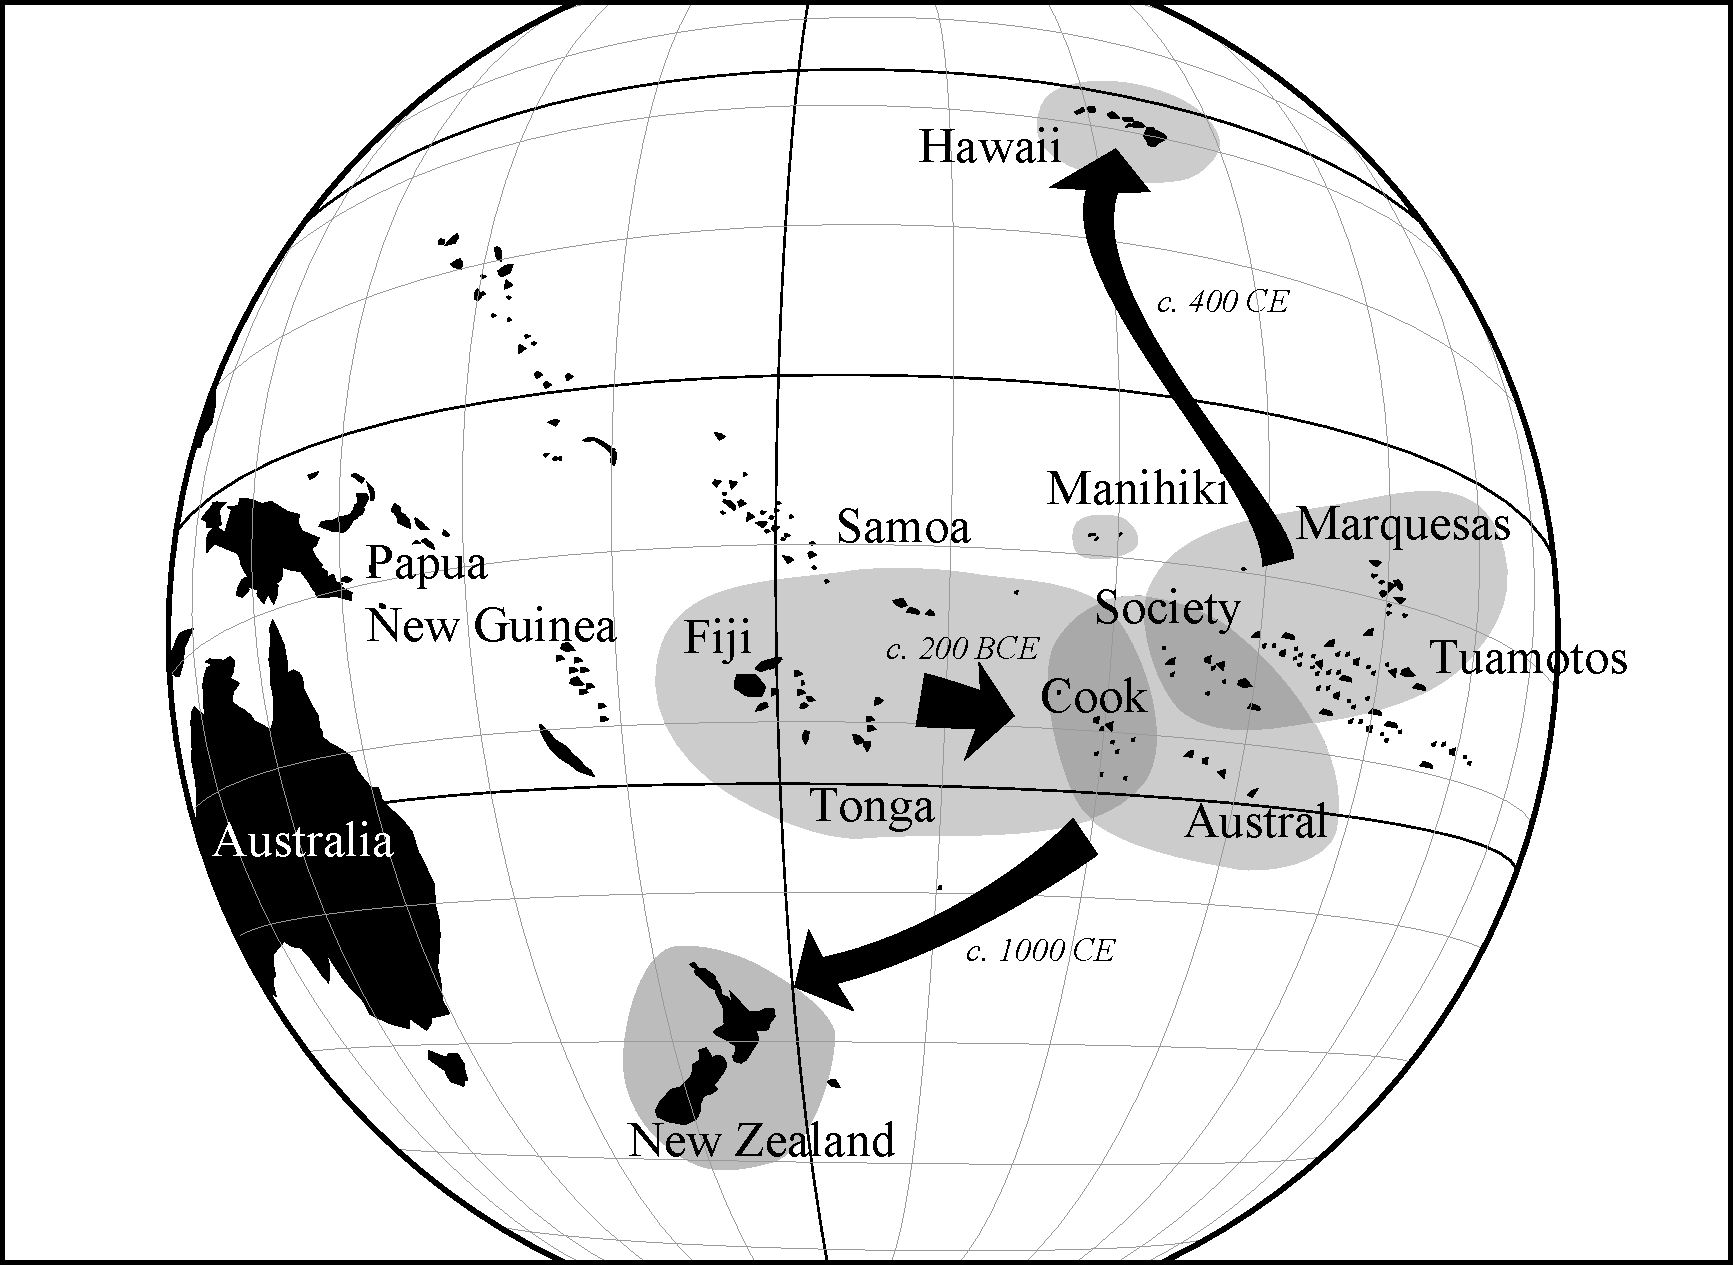
\includegraphics[scale=0.4]{figures/canoes/figMap.pdf}
    \end{center}
    \caption{\small Settlement sequence following Kirch \citeyearpar[black arrows]{Kirch2000:Road} and five major post-settlement interaction spheres (shaded regions) based on Weisler \citeyearpar{Weisler1998} in the eastern Pacific.}
    \label{map}
    \end{figure}
    
   Our models of Polynesian cultural inheritance focus on two forms of transmission: the inheritance of material culture via colonization, and the flow of information and material technology between established island societies.  Given that the exact island-to-island settlement sequence of Polynesia is still contested \citep{Kirch2000:Road, RogersFeldmanEhrlich2009}, we define it in broad, regional generalizations (Figure \ref{map}, black arrows).  Currently, it is established that the Polynesian settlers moved west to east through four major regions: first, the triangular region defined by Fiji, Samoa and Tonga, then onto the Cook, Society, Tuamotos, and Austral archipelagos making up Central Polynesia, and from there north to Hawaii and southwest to New Zealand.  Broadly speaking, these four regions can be considered a settlement sequence, and so canoe designs in one region may help predict canoe designs in the next region in the sequence.  Hawaii petroglyphs, for example, indicate that the Hawaiian crab-claw sail has a common ancestry with the Tahitian analog, and so knowledge about Tahitian canoes should presumably inform us about Hawaiian designs as well \citep{Lewis1978:PacificNavigators}.
   
   Post-settlement interactions between archipelagos also clearly played a role in shaping canoe designs.  The Fijian \textit{ndrua} double canoe, described by Haddon and Hornell as the ``largest and finest sea-going vessel ever designed'' in the Pacific, incorporated a shunting-capable rig\footnote{Shunting is an innovation for sailing against the wind unique to Oceanic seacraft in which the rigging is reversed so the fore becomes the aft and vis versa.  See chapter appendix for details.} from nearby Micronesia and in turn was the basis for the Tongan \textit{kalia} design and the Samoan \textit{'alia} design \citep[pg.~319]{HaddonHornell1936}.  Canoe diffusion was often very direct - Haddon and Hornell report that Society islanders would employ Tuamotoan canoe builders, who in turn imported Tahitian hulls \citep[pg.~74,79]{HaddonHornell1936}.  Weisler \citeyearpar{Weisler1998} presents evidence for six major interaction spheres in the South Pacific, defined by tracing basalt adzes back to their islands of origin using x-ray florescence techniques.  Using Weisler's geochemical diffusion data as a guide, we group the islands in our dataset into five general zones of interaction within which canoe technology might have been regularly shared (Figure \ref{map}, shaded regions).  Both inheritance from trading spheres and the island-to-island phylogenetic settlement sequence are included as covariates (see chapter appendix for specifications of each).

    
%-----------------------------------------------
\subsection{Models of Ecology}

    We must also consider the possibility that two societies will resemble each other simply because they exist in similar ecological environments, regardless of whether they interact with each other or share common ancestors.  As Kirch describes the experience of migrating Polynesians, ``Whether the new land was too isolated to maintain contacts with the homeland, whether it was vast or small, high or low, endowed with permanent streams, and so on, were factors that were to channel evolutionary pathways in certain directions.'' \citep{Kirch1984evolution}. Canoe builders may converge on hull designs again and again because of ecological pressures or the availability of certain critical resources.  For example, islands with protective reefs or atolls with enclosed lagoons allowed for relatively simple dugout designs with low freeboard, while open-ocean canoes necessitated raised washstrakes and weather screens.  The narrow Polynesian timber available for basic dugout canoe construction was easily capsized, and for anything but the calmest seas required a secondary stabilization mechanism in the form of an outrigger float or second hull.  Once Polynesians reached New Zealand, though, larger trees obviated the outrigger and double hull designs, both of which disappeared altogether after the cessation of regular long-distance voyaging.  Astronomical wayfinding techniques were lost, and Maori terminology specific to outrigger construction was either abandoned or repurposed to describe single-hulled Maori designs \citep{Biggs2006}.

The above motivates a number of ecological covariates.  Because the geological histories of island chains are effective proxies for many other ecological differences between Polynesian archipelagos \citep{Kirch2000:Road}, the elevation profile of an island (atoll, high island, or the coral-uplift \textit{makatea} island) and the presence or absence of a reef are included as ecological covariates.  Island area can be interpreted as a proxy for natural resource availability \citep{Banack1991ethnobotany}, the degree to which its inhabitants relied on trade with other islands for vital supplies, as well as a low-resolution measure of population density and carrying capacity.\footnote{The large size of both Hawaii and New Zealand provide dramatic examples of the effect of area on population size.  Even though New Zealand is more appropriately seen as a small continental remnant of Gondwana, we classify it as a high island because its elevation gradients bring similar advantages to the mountainous volcanic islands for canoe technology, such as more diverse and abundant plant and mineral resources.}  Ecological data were collected from descriptions in Mueller-Dombois and Fosberg \citeyearpar{Mueller1998:Vegetation} and through a cross-Oceanic survey using satellite images from Google Earth.          

%-----------------------------------------------
\subsection{Model Specification and Estimation Using Bayesian Statistics}

    Using these ecological and cultural covariates, we specified 27 logistic regression models to compare using model selection techniques, divided into four broad categories: null models (N), models incorporating cultural inheritance (C), ecology (E), or both (CE, see the chapter appendix for the details of model specification). The large number of models reflects the fact that environmental and cultural inheritance predictors can influence canoe design in many ways; there is no general theory constraining the structure of these models.

If $i \in {1,2,\dots ,11}$ indexes island group and $t \in {1,2, \dots , 65}$ indexes canoe traits, then the binary variable $x_{t,i} \in \{0,1\}$ describes the presence or absence of trait $t$ on island group $i$ for the 65 $\times$ 11 matrix of island traits $X$. Since the goal is to predict $x_{t,i}$, the general form of each model is
    \[\mathrm{Logit} \Pr( x_{t,i}=1 ) = \alpha_t + Z_i B,
\]
where $Z_i$ is a vector of ecological and cultural inheritance covariates for island $i$ and $B$ is a vector of coefficients. We know beforehand that different traits likely do not occur with the same baseline frequency (the intercept in a logistic regression model), so we need to estimate a frequency, $\alpha_t$, for each trait (see chapter appendix). The need to model variation in a large number of traits suggests a model with a large number of parameters, yet the number of island groups represented is relatively small. The classic frequentist approach is unsuitable under these conditions because there is too little data and consequently too few degrees of freedom to fit a large model. We solve this problem by using a single prior distribution for all $\alpha_t$, resulting in models containing 1 to over 150 parameters. This allows us to make a relatively parsimonious model for baseline frequencies, yet permits frequencies to vary across traits.

Because little or no prior information is available, we assign Gaussian priors with high variances to all parameters. The prior for $\alpha_t$ has a mean of zero and a variance of 10, whereas all other parameters have prior variances of 100 (see Box~1 in the chapter appendix for common terms in Bayesian statistics). Using a Gibbs sampler implemented in the software \texttt{R} and \texttt{Winbugs}, we estimate posterior distributions and the Deviance Information Criterion (DIC), an analog to the more common AIC and BIC for Bayesian model selection\cite{Spiegelhalter2002, Gill2008}.  For logistic regression there is no true equivalent of $R^2$, the proportion of variance in the data explained by the model. Instead we compare our models' performance to ``benchmark'' or null models. Two null models, one with a constant intercept across all traits and islands (`Weighted coinflip') and no covariates, and another having an intercept for each trait (`Base', again without other covariates) are included to compare the added predictive power of models with ecological and inheritance covariates.


%----------------------------------------------    
\section{Results}
%-----------------------------------------------

    \begin{figure}[t]
    \begin{center}
      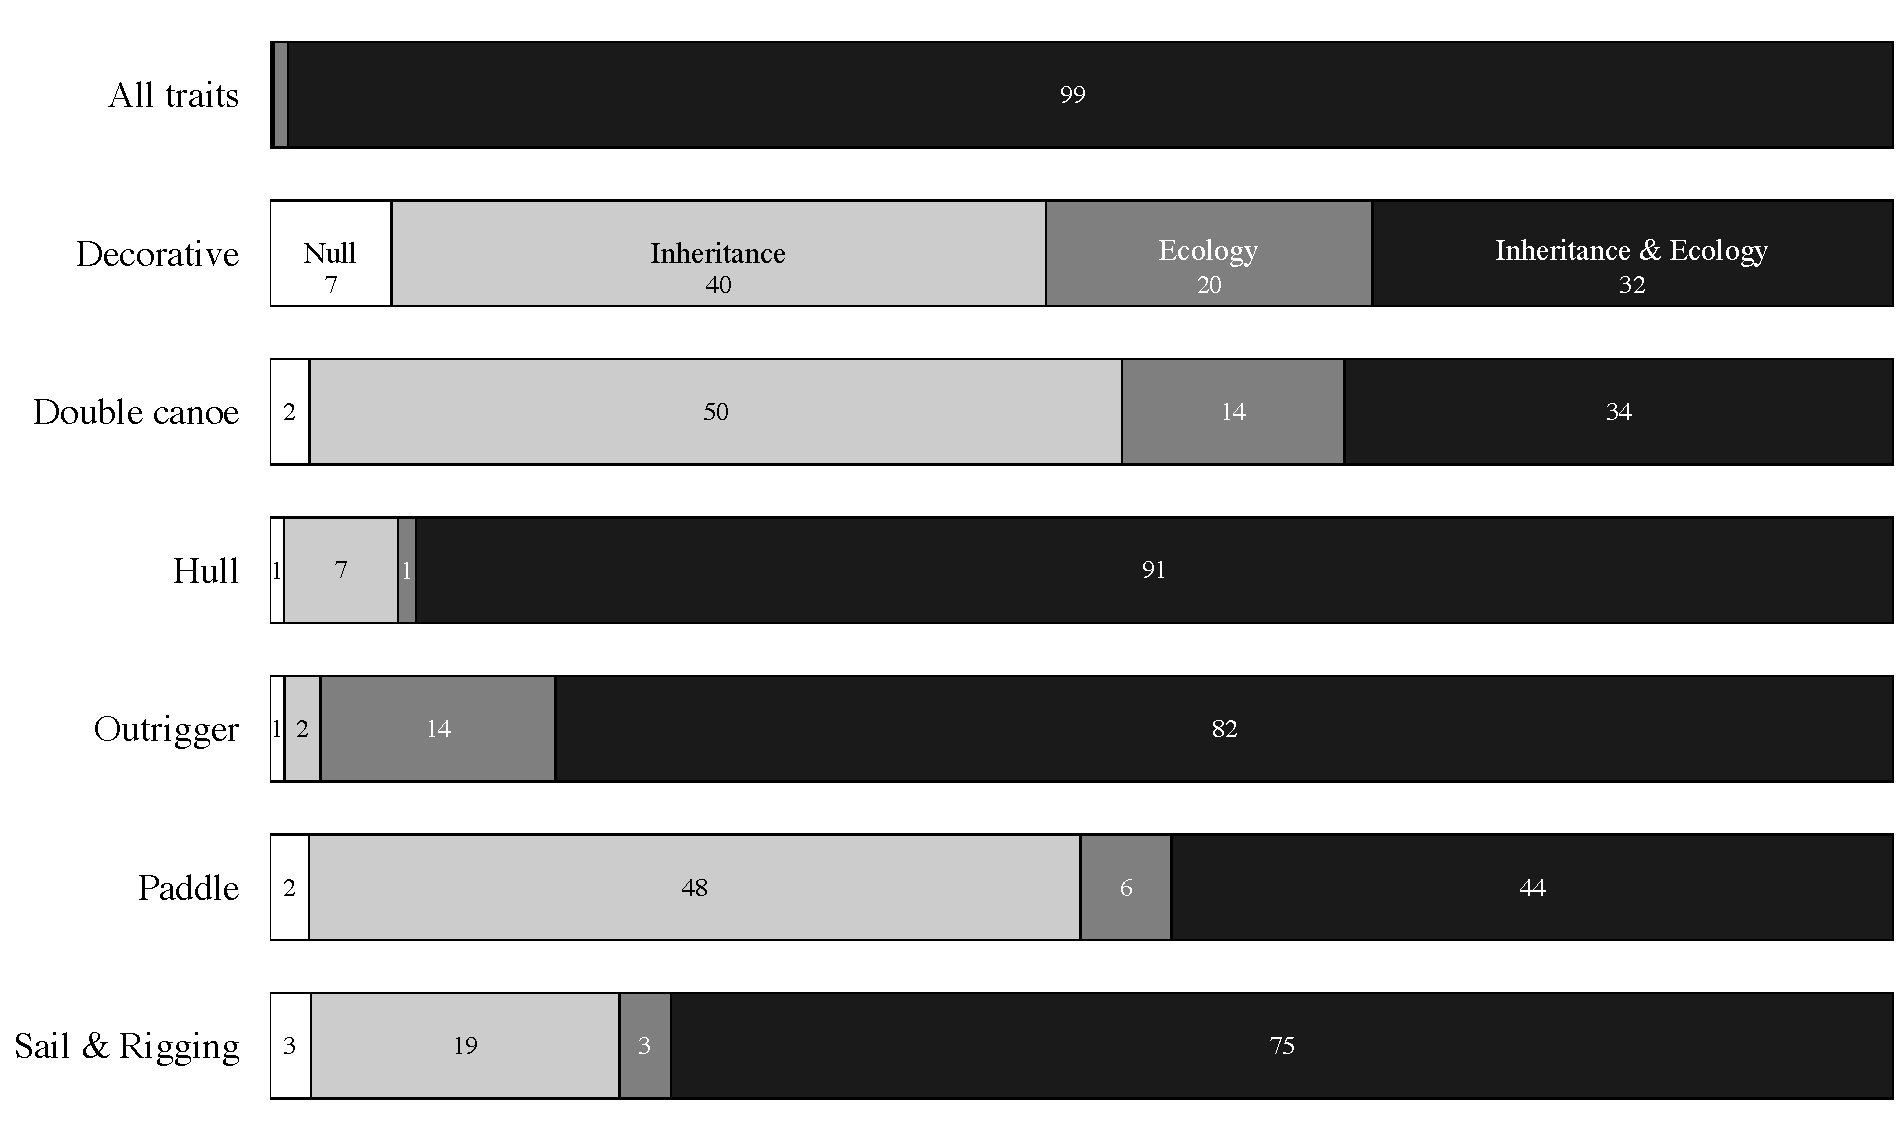
\includegraphics[scale=0.45]{figures/canoes/figBars.pdf}
    \end{center}
    \caption{Plot of the relative weight assigned to the four classes of models (where whitespace represents null models).  Size of each colored region represents the sum of DIC weights attributed to that class of models, characterizing the relative weight of evidence in favor of that class of model \citep{Burnham&Anderson:2002}. The wider a specific region the more likely the corresponding class of models describes the process behind the evolution of that particular set of canoe traits. If no region is dominant, there is less certainly or the models explain very little. }
    \label{barplot}
    \end{figure}
                         
We classify 65 distinct canoe traits for 11 island groups into six general categories: hull design, decoration, rigging, paddles, outrigger traits and double-hulled canoe traits (see chapter appendix for details).  DIC scores were calculated for each of the 27 models fitted to the full dataset, and separately fitted to each of the six trait subsets.  Since these scores are only meaningful in relation to those of other models, a given model's absolute score is less important than its relative distance to the top model's score ($\Delta$ DIC) and the model's information criterion weight, $w$.  The results of each analysis are presented in Figure \ref{barplot}, which measures the relative explanatory power of models that included only ecological covariates (E), covariates of cultural inheritance (C), both (CE), and the two null models.  

%-----------------------------------------------


    \begin{figure}[t]
    \begin{center}
      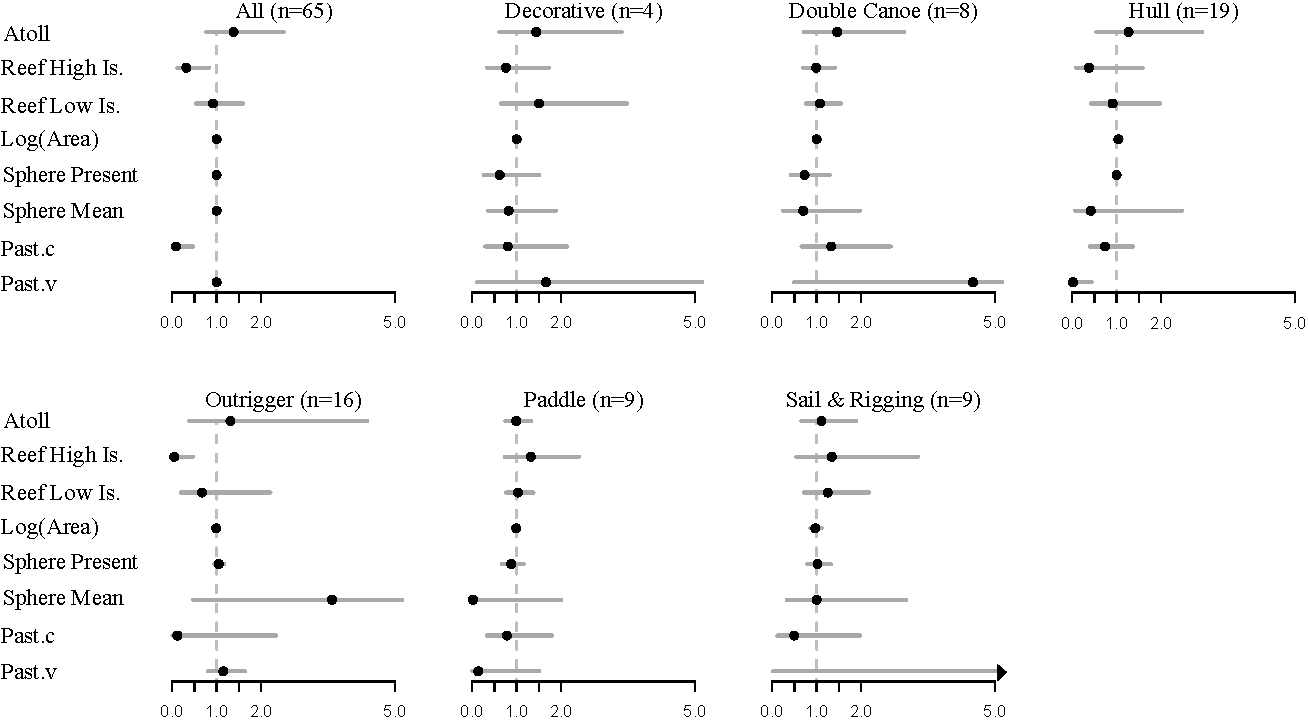
\includegraphics[scale=0.65]{figures/canoes/figOR.pdf}
    \end{center}
    \caption{Model-averaged odds-ratio estimates with 95\% Upper and Lower bounds for eight covariates.  The first three covariates estimate the effects of modal properties of the island group; whether or not the islands are atolls, high islands with reefs or low islands with reefs.  The remaining four covariates describe an island group's cultural ancestors and neighbors; ''sphere present'' and ''sphere mean'' consider the presence and frequency, respectively, of each canoe trait within trade interaction spheres, while ''past.c'' and ''past.v'' consider the presence of each canoe trait among island groups earlier in the settlement sequence, using constant or trait-varying imputed values, respectively, for the first island group in the sequence (see chapter appendix).}
    \label{ORresultsfig}
    \end{figure}
 
%--------------------------------------   
 \subsection{Model rankings}   

Considering all canoe traits, models that include both cultural and ecological (CE) covariates consistently outperform those including either covariate category alone.  When considering all 65 traits, the top four models, all CE, constitute 99\% of the total DIC weight. Among the CE class of models, those that consider island settlement sequence, island area, and geological type of island perform the best (see chapter appendix). The top model with 67\% of the total weight considers only settlement sequence and island type.  The second model at 27\% of the weight has the same covariates as the top model but with the addition of the log(area) covariate. Finally, the third ranking model adds trade spheres, though because its weight is only 4\%, post-settlement interactions between islands are less useful on average across these data.

This basic pattern is also found for traits specific to the canoe's hull, sail and rigging, and traits specific to outriggers; CE models of one form or another rank the highest and take up the majority of the model weights in each subcategory.  The top model for hull traits, with 41\% of the model weight, includes settlement sequence, area, and island type. The next best (18\%) includes trading partners and drops island type, together covering all four covariate categories.  Considering sail and rigging traits, CE models rank highest, but the top models carry roughly equal weight, indicating equivalent explanatory utility.  For outrigger traits the top model at 42\% weighting includes island type and settlement sequence, and the second ranked model (26\%) adds log(area) and trading spheres. 

While models that include only cultural inheritance covariates occasionally outperform the composite CE models, though the same cannot be said for ecology models or the null models.  These C models dominated the rankings for paddle traits (Figure~\ref{barplot}), whose top model considers only settlement sequence and trading spheres, both present in nearly all models that outperformed the null.  For double-hull canoe traits, C models take up the majority of model weights, though among them there is no clear winner.  

The models rankings for decorative traits are in contrast to those of all other trait subsets.  The top two models consider only covariates of cultural inheritance, constituting 13\% and 11\% of model weight, respectively.  However, the third ranking model, at 7\%, is the null model Base, followed by CE and E models all at around 6\% of model weight.  In general the model weights for decorative traits are distributed among CE, C and E models roughly equally (Figure \ref{barplot}).  We interpret the inability to distinguish a clear winner and the prominence of the null model as evidence of poor performance among all our models, and so none are particularly compelling explanations the observed variation in canoe decoration \citep{Burnham&Anderson:2002}.  
 

%--------------------------------------   
 \subsection{Effects of single covariates}   

We also report model-averaged odds-ratios (see chapter appendix for discussion on model-averaging methods). Primarily, the estimates reflect the uncertainty in predicting canoe traits using any one particular covariate (the dimensions of our sample are 11 islands by 65 traits, suggesting only sparse information). Most estimates have lower and upper bounds that include 1.0, the value of ``no effect'', though the posterior means of many estimates are far from one.  However, while some covariates may have imprecise point estimates (broad posterior distributions), they do in many cases contribute to a model's performance in the above model rankings.  Despite estimate uncertainty, model selection methods can still be used to make inferences.  

Some of the more precise and contrasting estimates are worth noting (Figure \ref{ORresultsfig}). The ecological covariate ``Reef High Is.'', a dummy variable for this island profile, has a negative effect on all canoe traits taken together, and specifically outrigger and (more ambiguously) hull traits.  In terms of the odds ratio, any given canoe trait is much less likely to be present on high, reefed islands than when island type is unknown.  

We also estimate strong negative predictive effects for settlement sequence covariates for a variety of canoe traits, meaning that they are less likely to be present on an island group if those traits are present or common in the ancestral region of the Pacific that settled that island group.  Specifically, covariate ``Past.c'' has a negative predictive effect on canoe traits in general and a (more ambiguous) negative effect on outrigger traits.  The other settlement sequence covariate, ``Past.v'', has a particularly strong negative effect on hull and paddle traits.  (We consider the effect strong because the mean estimate is far from one and a relatively small portion of the total interval extends across one).  We registered only two estimates of positive effect on the odds ratio, both ambiguous; settlement sequence (``Past.v'') on double canoe traits, and trading spheres (``Sphere mean'') on outriggers.  


%-----------------------------------------------
\section{Discussion}
%-----------------------------------------------

Taken together, these results tell an interesting story about Oceanic canoe designs.  The majority of focal canoe traits are best explained by settlement sequence and island type; there is little to no evidence that island land area or inter-island trade enhances our understanding of canoe trait distribution.  When clear, the estimated effects of settlement sequence and island type are also strongly negative - our models predict that the settlement of high, volcanic islands with reefs is followed by the disappearance of these canoe traits.  This is particularly true for outrigger and hull designs.    

Exactly why the settlement of high, reefed islands is associated with the absence of our focal canoe traits is an open question.  Of the eleven island groups considered, two of the largest (Hawaii and New Zealand) have the fewest canoe traits (24 and 23 traits, respectively, out of 65).  However, Fiji, by land area larger than Hawaii, has 34 traits, one of the highest in the sample.  As a result, while models including the log of island area are among the top ranked, the estimated effect of island area on the odds ratio is negligible.

Instead of land area, our high island covariate may be capturing the effects of greater natural resources available on high islands; Maori designs in New Zealand could use trees so massive double-hull and outrigger designs were no longer necessary, while canoe builders on low islands like the Tuamotos had to work with lashed planks in lieu of simple dugouts.  Indeed, many of the focal canoe traits in our sample can be seen as adaptations to low-resource environments, and so it may be expected that these would be abandoned upon the ecological release of reaching Hawaii and New Zealand.  

Another possibility is the effects of population size on canoe design.  Henrich \citep{Henrich2004:Tasmania} demonstrates how sampling error in low population sizes can cause the decay and eventual disappearance of useful technology, such as observed on Tasmania.  The process on New Zealand and Hawaii may be roughly the opposite - massive technological undertakings that require state-like centralized political authority and the collective knowledge of large networks of canoe designers may rapidly replace technological designs that can be sustained within smaller founding populations.  

Both hypotheses imply that a key influence on the results is the processes about \textit{which} canoe traits are recorded and coded.  This is a important methodological point, as two subsequent analyses \citep{RogersFeldmanEhrlich2009,GrayBryantGreenhill2010} have been carried out on the Rogers and Ehrlich \citeyearpar{Rogers2008:Canoes} dataset, and the results of each may be sensitive to alternative coding.  From the descriptions of Haddon and Hornell, among others, New Zealand and Hawaii clearly do not have a dearth of canoe designs.  However, because the focus of anthropological analysis is the flow of canoe designs across Polynesia, variations in canoe technology unique to these end-sequence islands groups may be underrepresented in the analyses.  Using our methods, future work that includes a greater emphasis on the diversity of canoe technology on high volcanic islands, as influenced by population size and natural resource constraints, should be able to provide an answer on this issue.

Though there are good theoretical reasons to think these methods reliably extract information from the data at hand, those results must be evaluated in light of prior knowledge about the historical record.  Since there is strong evidence from oral histories that shunting-capable sailing rigs spread from Fiji through a settled Polynesia, the fact our models do not nominate inter-island trade in the ``sail and rigging'' analysis may say more about our sample and coding procedures than the actual diffusion of canoe technology.  Likewise, other covariates that better capture neutral drift and the dynamics of ethnic markers may prove to be more effective at explaining the distribution of decorative traits. 

Despite these reservations, our results present clear quantitative evidence that statistical models incorporating both ecological and cultural inheritance covariates are better explanations of Oceanic canoe designs than either alone.  Moreover, using these methods we are able to elucidate interesting patterns in the historical record without arguing for or against particular evolutionary processes.  Our analysis provides support for the inclusion of both social-historical and ecological perspectives in the study of Polynesian seafaring, and demonstrates a method by which historians and anthropologists can test hypotheses of cultural change through the direct comparison of formalized statistical models.  

\newpage
\section{Appendix to Chapter 1}


\subsection{Canoe Supplement}

\begin{figure}[ht]
\begin{center}
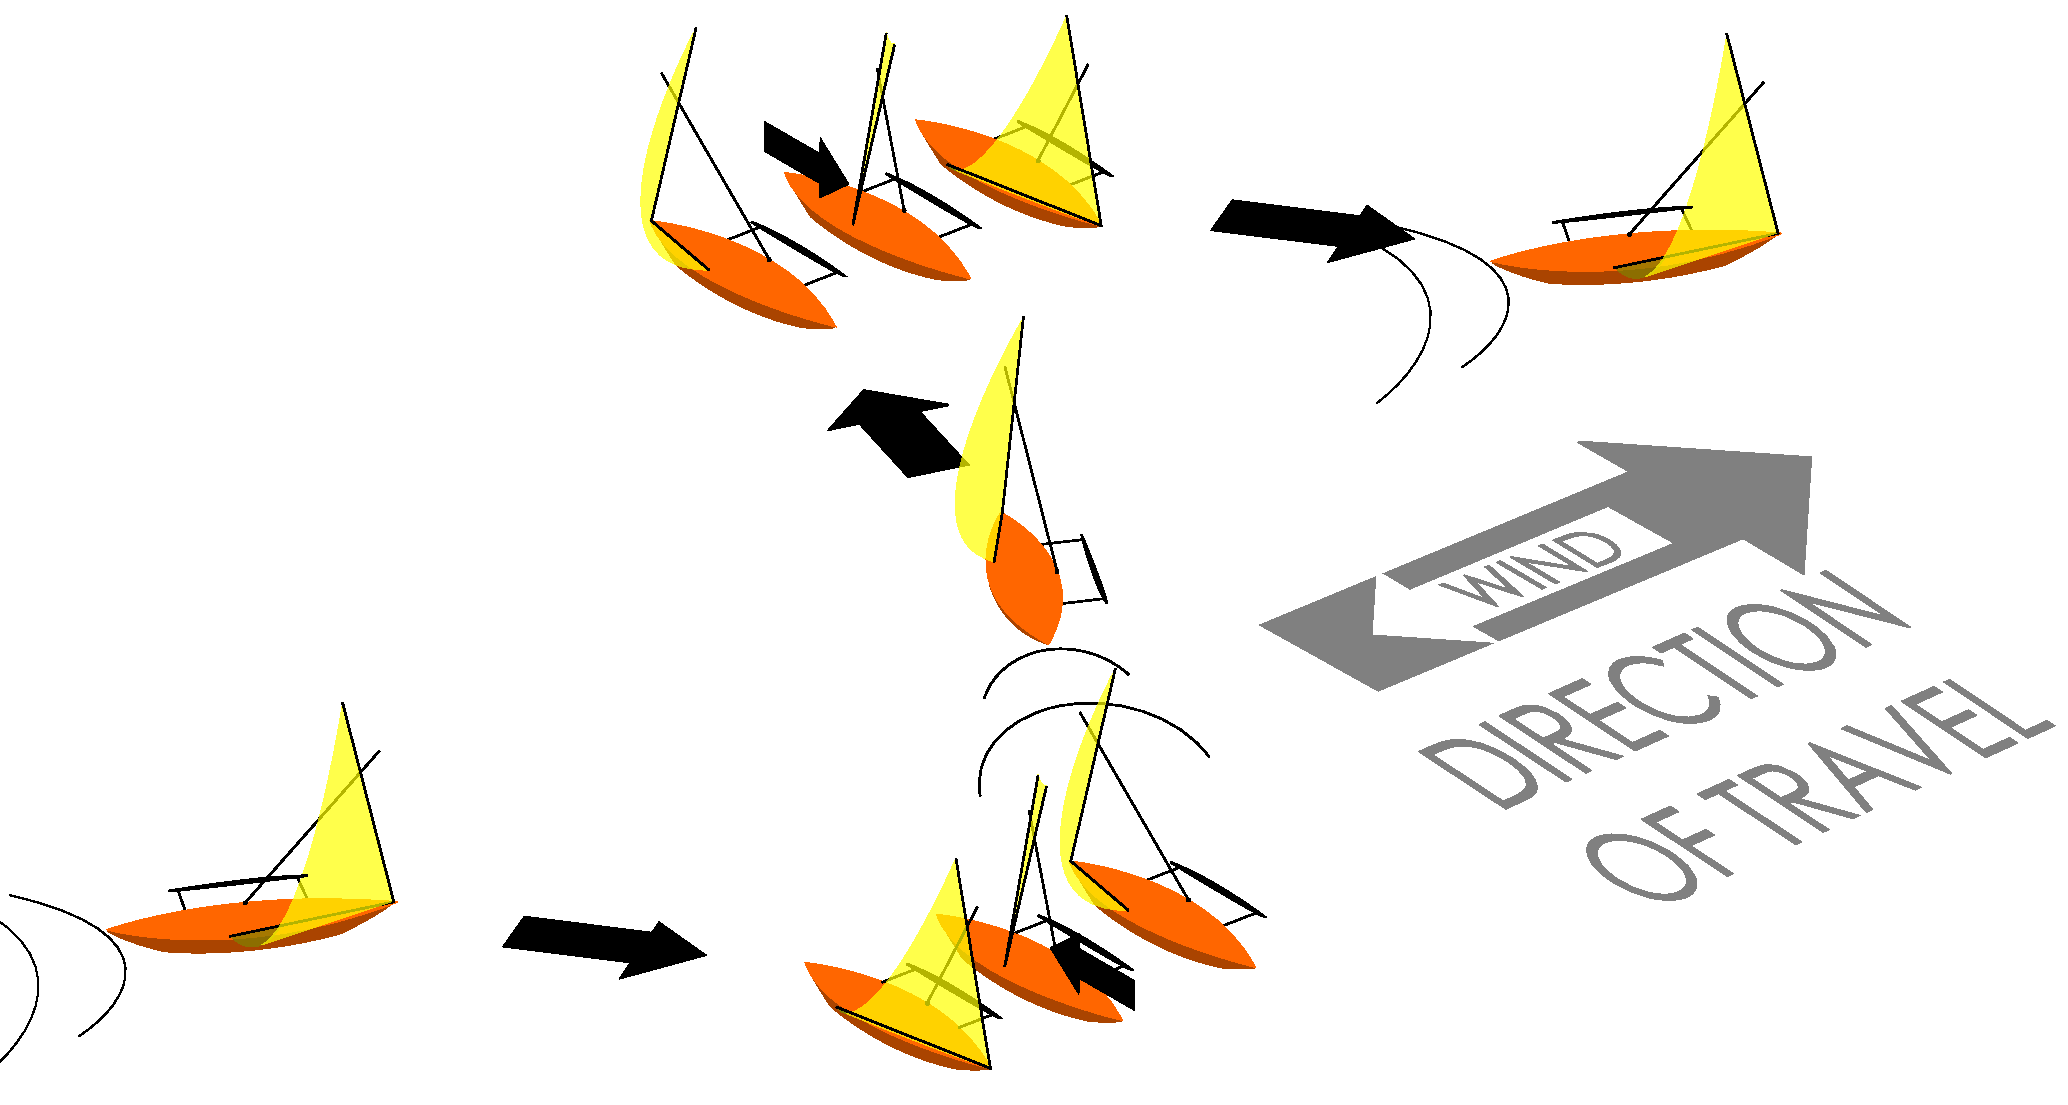
\includegraphics[scale=0.45]{figures/canoes/ESMFigure1.pdf}
\caption{Illustration of shunting procedure.  This technique for moving upwind involves turning the canoe at a right angle from the prevailing wind, manually lifting the tack out of its fore socket, and carefully walking it to the other end of the canoe to insert in an equivalent socket in the aft, reversing the direction of sailing.}
\end{center}
\end{figure}

\begin{figure}[ht]
\begin{center}
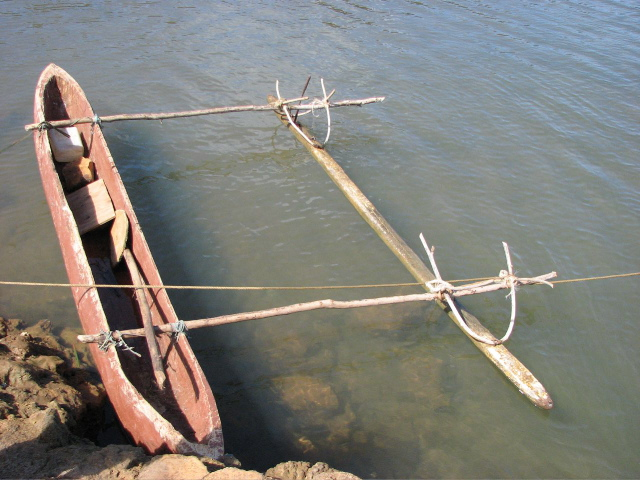
\includegraphics[scale=0.4]{figures/canoes/ESMFigure2.jpg}
\caption{Tongan dugout with outrigger.  Two booms and indirect U-shaped stanchions connect main hull to outrigger float.  Low freeboard (distance between waterline and gunwale) and lack of washstrakes (added planks along sides to keep the sea out) make this canoe more vulnerable to swamping compared to that in Figure 3.  \textit{Photo by A.V. Bell. }}
\end{center}
\end{figure}

\begin{figure}[ht]
\begin{center}
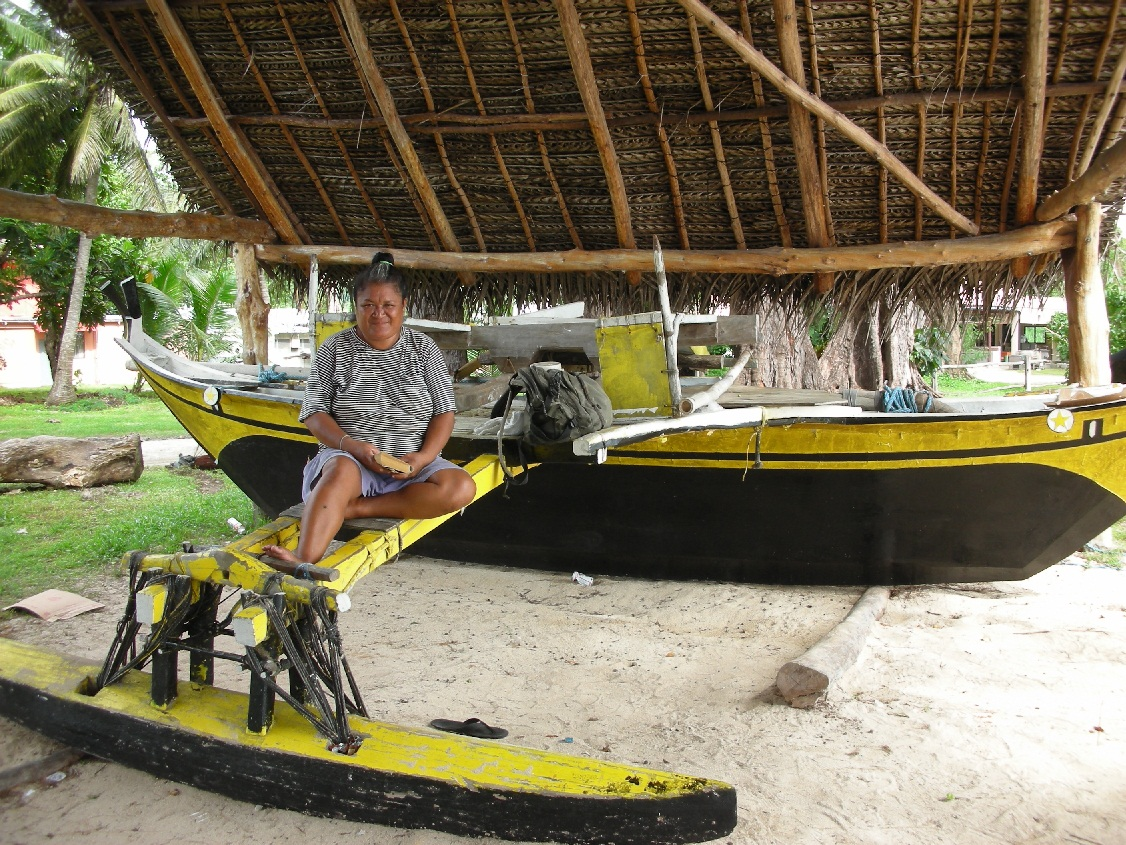
\includegraphics[scale=1]{figures/canoes/ESMFigure3.jpg}
\caption{Micronesian outrigger.  \textit{Photo by Kathryn Demps.}}
\end{center}
\end{figure}

\newpage
\subsection{Model Selection Methods}

The deviance information criterion is
 \[ DIC = -2 \overline{\log(\mathcal{L}(\widehat{\theta}))} + 2p_D
\]
where $\overline{\log(\mathcal{L}(\widehat{\theta}))}$ is the average deviance over 100,000 simulations using WinBUGS and $p_D$ is the effective number of parameters.  The relative distances, rather than absolute magnitudes, of the DIC scores of the models are the basis for comparing them, and so it is common to report each model�s $\Delta$ DIC relative to the top model (with the lowest DIC score).  Among all R models used in the model comparison, DIC weights are calculating for model $i$ with associated $\Delta$ DIC $d_i$ via
\[w_i = \frac{\exp(-0.5 d_i)}{\sum_{r=1}^R exp(-0.5 d_r)}
\]
Rather than report the parameter estimates from a particular model, we can use the DIC weights and parameter estimates of all models to create model-weighted estimates (Burnham and Anderson, 2002).  Specifically, the vector of model-weighted estimates across a set of R models is given by
  \[\widehat{\overline{\theta}} = \sum_{i=1}^R w_i \widehat{\theta}_i
\]
where $\theta_i$ is the estimate of parameter $\theta$ for model $i$, $w_i$ is the DIC weight for model $i$, and $\widehat{\overline{\theta}}$ is the model-averaged estimate of $\theta$.  Model-weighted variance is calculated in a similar way, save for an additional term to account for the uncertainty among models (Burnham and Anderson, 2002), yielding
  \[\widehat{var}(\widehat{\overline{\theta}}) = \left[\sum_{i=1}^R w_i \sqrt{\widehat{var}(\widehat{\theta_i}|g_i) + (\widehat{\theta}_i - \widehat{\overline{\theta}})^2}\right]^2
\]

%
%
%%-----------------------------------------------
%\subsection{Further Reading}
%%-----------------------------------------------
%Pacific societies have attracted generations of anthropologists and ecologists for their ability to serve as natural ``laboratories'' of human behavior and socio-ecological processes \cite{Mead1957:PolynesianLab}, and are particularly useful for testing models of cultural transmission and behavioral ecology.  Because settlers generally moved west-to-east from the ancestral Lapita homeland in the Bismarks and Solomons, and long-distance voyaging between archipelagos ceased by 1450 CE \cite{Weisler2002:LongVoyagingCollapse}, Pacific island settlements provide an unusually well-partitioned phyletic distribution of cultural variation \cite{KirchGreen2001}.  In fact, the isolation of some Polynesian communities has led to cultural divergences that mirror those of the endemic fauna that surround them, allowing anthropologists to use phylogenetic language trees to infer settlement sequences \cite{Gray2000tree, Gray2009:Phylogenies}. On the other hand, it is well understood that ecological conditions played a determining role in the fates of many Pacific societies, and recent Oceanic archaeology has focused on how chemical, biological and climatological gradients both structure and are themselves shaped by agrarian landscapes and socio-political systems \cite{Kirch1984evolution, Kirch2007}.
%
%Within the last fifty years, models of human settlement and dispersion in Fiji and Polynesia have become increasingly ecumenical, supplementing archeology and traditional ethnography \cite{Anderson2006motivation,Feinberg1988seafaring} with structuralist social theory \cite{Sahlins1985:History}, climatology \cite{Anderson2006ENSO}, geochemistry \cite{Collerson2007adze}, genetics \cite{MatisooSmith2004:PacificRatDNA, Whyte2005:PolyHumanEvol, Friedlaender2008:PacificGenetics}, linguistics \cite{Greenhill2005:DispersalTrees}, computational modeling \cite{DiPiazza2007virtualcanoes, Avis2007discovery}, and, in the case of Ben Finney's double-hull \textit{Hokule'a}, experimental seafaring \cite{Finney1994:Rediscovery}. Although the peopling of the Pacific has captured the attention of centuries of scholarship, debates continue about (1) how purposive Polynesian voyaging was \cite{Whyte2005:PolyHumanEvol}, (2) the sequence and methods of settlement \cite{Irwin1992}, (3) how quickly it occurred \cite{Anderson2000:Slowboats, Thomas2008:Lastpulse, Gray2009:Phylogenies}, (4) the extent of pre-European trade and interaction  \cite{Weisler1998}, (5) the kinds of canoes and sailing rigs employed in these processes \cite{Doran1981canoes, Anderson2001:SharpEnd}, and (6) the evolutionary pressures that shaped them \cite{Horridge1987:IndonesiaCanoes}.
%-----------------------------------------------
\subsection{Data Reprocessing}
%-----------------------------------------------



Our dataset classified 65 distinct canoe traits based on descriptions in Haddon and Hornell's \textit{Canoes of Oceania}.  Beginning with Rogers and Ehrlich's (2008) 134-trait dataset, we excluded or merged traits which were most likely to be affected by recording biases, practical dependencies and coding errors.

For example, although encyclopedic in their treatment, Haddon and Hornell employ an inconsistent use of certain terms, such as \textit{sennit} and \textit{coir}, whose distinctiveness is critical to traits coded as OAH12, OAH13 and DAH11.  In such cases, traits were merged to eliminate the potential for artificial distinction.  

Additionally, since many of the descriptions in \textit{Canoes of Oceania} were culled by Haddon and Hornell from a hodgepodge of accounts by European explorers, missionaries, merchants, and scholars over a period of several hundred years, the potential for simple omission of a canoe trait actually present on an island group is considerable.  That Fijian double canoes ranged from 25 to 72 feet in length, 97 to 120 feet in length, but not in-between suggests the presence of a ethnographic sampling bias, rather than some actual design preference or constraint.  

In some cases, the supplementary table in Rogers and Ehrlich (2008) is clearly missing data; use of Hawaiian canoes for fishing was coded as ``absent'' (OCP2, DCP2), even though both double-hull and outrigger canoes had fishing-pole rests (OAF1, DAF1).  Similarly, though outrigger canoes were common in both the Australs and Tonga, traits OAO1 (``Outrigger present on port side'') and OAO2 (``Outrigger present on starboard side'') are both coded as ``absent'' for these archipelagos, a logical impossibility.  Coding the orientation of the outrigger floats is particularly problematic because Polynesian canoes were often designed to sail with either end facing forward and have no permanent starboard and port, rendering such traits essentially meaningless.  To circumvent this problem, we excluded traits likely to be missing data points or whose presence in the island group was ambiguous among the primary sources.

Furthermore, several traits were excluded because of likely influence of practical interdependencies, invisible to covariance screening tests because of potentially large sampling biases and the confused nomenclature in \textit{Canoes of Oceania}.  For example, ``mast stepped forward'' and ``Oceanic Lateen sail present'' are treated in the original dataset as independent traits, despite the fact that the former is a necessary component of the latter \citep{Doran1981canoes}.  Doran's survey of Austronesian canoe designs synthesizes a variety of reports by Haddon and Hornell into distributional maps, and also provides the basis for our data on the distribution of shunting and the use of the primitive crane sprit.      

Finally, we compacted equivalent double-hull traits and outrigger traits, on the premise that any discrepancies between the two categories represent noise rather than useful information.  Considering the regularity by which outrigger and double-hulled canoes were converted from one to the other in Polynesia, the notion that traits on one canoe type should be distinct from traits on the other does not appear tenable.


\subsection{Model Specification and Estimation}

We introduce some notation to describe trait distributions and our models. Let $i \in \{1,2, \dots ,11\}$ index island group and $t \in \{1,2,\dots,65\}$ index canoe traits. Then binary variable $x_{t,i} \in \{0,1\}$ describes the presence or absence of trait $t$ on island group $i$ for the 65 $\times$ 11 matrix of island traits $X$.

Using the currently understood colonization sequence (see Figure 1 of the main text), let $C_i$ be the set of island groups within the region that colonized island group $i$, and $|C_i|$ be the number of island groups in $C_i$. Now, the frequency of trait $t$ in the colonizing region $C_i$ of island group $i$ is $y_{t,i} = \left( \sum_{j \in C_i} x_{t,j} \right) / |C_i|$. Now let $S_i$ be the set of island groups within the sphere of influence of island group $i$, based on the zones of interaction compiled by Weisler (1998), and $|S_i|$ be the number of island groups in $S_i$. Then the frequency of trait $t$ in the sphere of influence $S_i$ of island group $i$ is $m_{t,i}= \left(\sum_{j \in S_i} x_{t,j} \right) / |S_i|$. Because data sources are not properly collected statistical samples in any sense, we should consider that the presence of a trait in a region is more diagnostic for cultural transmission than its observed frequency (as recorded in Haddon and Hornell (1936)). Hence, for interaction spheres, we also consider sphere presence/absence models using $p_{t,i}= 1$ if $m_{t,i}>0$, and $0$ otherwise.

Since the goal is to predict $x_{t,i} \in \{0,1\}$, the general form of the model for trait $t$ is
    \[\mathrm{Logit} \Pr( x_{t,i}=1 ) = \alpha_t + B Z_i \],
where $Z_i$ is a vector of ecological and cultural inheritance covariates for island $i$ and $B$ is a vector of coefficients. Table~\ref{modeltable} shows examples of null (N) models, cultural inheritance (C) models, ecological (E)  models, and the cultural inheritance-ecological (CE) models.

Using a Gibbs sampler implemented in the software \texttt{R} and \texttt{Winbugs}, we estimate posterior distributions and the Deviance Information Criterion (DIC). For each run of the Gibbs sampler we perform 100,000 interations with a burn-in of 50,000 interations. Starting values for continuous parameters were randomly drawn from a Gaussian distribution with mean zero and variance 1, and binary parameters randomly drawn from a Binomial distribution with the probability of a success (drawing a value of one) equal to one-half.

    \begin{table}[t]
    \begin{center}
    \begin{footnotesize}
    \begin{tabular}{p{7.5cm} p{7cm}}
    \bf{Model name} & $ \text{Logit }Pr(x_{t,i}=1) =$\\
    \hline
    {\em Null models}& \\
    \hline
    N1: Weighted coinflip & $ \alpha $ \\
    N2: Base & $ \alpha_t $ \\
    \hline
    {\em Inheritance} & \\
    \hline
    C1: Past & $\alpha_t + \beta_1 y_{t,i}$ \\
    C2: Past \& Sphere Present & $\alpha_t + \beta_1 y_{t,i} + \beta_2 p_{t,i} $ \\
    \hline
    {\em Ecology} & \\
    \hline
    E1: Island area &  $\alpha_t + \beta a_i$ \\
    E2: Reef high \& low \& Atoll & $\alpha_t + \kappa_1 r_{h,i} + \kappa_2 r_{l,i} + \kappa_3 r_{a,i}$ \\
    \hline
    {\em Inheritance \& Ecology} & \\
    \hline
    CE1: Past \& Area & $\alpha_t + \gamma y_{t,i} + \beta a_i$ \\
    CE6: Past \& Sphere Present \& Area \& Island type & $\alpha_t + \gamma y_{t,i} + \lambda p_{t,i} + \beta a_i + \kappa_1 r_{h,i} + \kappa_2 r_{l,i} + \kappa_3 r_{a,i}$ \\
    \hline
    \end{tabular}
    \end{footnotesize}
    \end{center}
    \label{models}
    \caption{Representative models of those considered in this analysis. The average island size in the focal archipelago ($a_i$), and ``Island Type'' represents ``Reef high'' ($r_{h,i}$), ``Reef low'' ($r_{l,i}$), or ``Atoll'' ($r_{a,i}$). \label{modeltable}}
    \end{table}

%-------------------------


% all traits
\begin{table}
\begin{center}
\begin{tabular}{lllll}
Models & DIC & $\Delta$ DIC & $w$\\
\hline
mPast2ReefHighLowAtoll & 944.75 & 0 & 0.67\\
mPast2AreaReefHighLowAtoll & 946.56 & 1.81 & 0.27\\
mPast2SpherePresentAreaReefHighLowAtoll & 950.43 & 5.68 & 0.04\\
mPast2Area & 953.01 & 8.26 & 0.01\\
mReefHighLowAtoll & 954.64 & 9.89 & $<$0.01\\
mReefHighAtoll & 955.35 & 10.6 & $<$0.01\\
mPast2SphereMeanAreaReefHighLowAtoll & 956.23 & 11.48 & $<$0.01\\
\textbf{mBase} & \textbf{957.57} & \textbf{12.82} & \textbf{$<$0.01}\\
mPast2SphereMeanArea & 958.33 & 13.58 & $<$0.01\\
mPast2 & 958.46 & 13.71 & $<$0.01\\
mArea & 959.5 & 14.75 & $<$0.01\\
mSphereMean & 959.78 & 15.03 & $<$0.01\\
mSpherePresent & 960.57 & 15.82 & $<$0.01\\
mAreaReefHighAtoll & 960.81 & 16.06 & $<$0.01\\
mAreaReefHighLowAtoll & 963.3 & 18.55 & $<$0.01\\
mPast2SpherePresentArea & 965.16 & 20.41 & $<$0.01\\
mPastReefHighLowAtoll & 969.62 & 24.87 & $<$0.01\\
mPastSphereMeanAreaReefHighLowAtoll & 971.35 & 26.6 & $<$0.01\\
mPastSpherePresentAreaReefHighLowAtoll & 978.44 & 33.69 & $<$0.01\\
mPastAreaReefHighLowAtoll & 981.08 & 36.33 & $<$0.01\\
mCoinFlip & 989.51 & 44.76 & $<$0.01\\
mPastSphereMeanArea & 1022.93 & 78.18 & $<$0.01\\
mPastSpherePresent & 1027.01 & 82.26 & $<$0.01\\
mPastSpherePresentArea & 1033.41 & 88.66 & $<$0.01\\
mPastSphereMean & 1037.35 & 92.6 & $<$0.01\\
mPastArea & 1047.06 & 102.31 & $<$0.01\\
mPast & 1048.18 & 103.43 & $<$0.01\\
\end{tabular}
\end{center}
\caption{Model rankings for all canoe traits. $\Delta$ DIC is the difference between a model's DIC score and the top model's, and DIC weights ($w$) quantify the relative performance among models.  The best-performing null model is highlighted in bold; models with higher rankings (lower DIC scores) are plausibly better at explaining the data than the null model.
\label{resultstable1}}
\end{table}



% decorative
\begin{table}
\begin{center}
\begin{tabular}{lllll}
Models & DIC & $\Delta$ DIC & $w$\\
\hline
mSpherePresent & 55.69 & 0.00 & 0.13\\
mPastSpherePresent & 56.11 & 0.42 & 0.11\\
\textbf{mBase} & \textbf{56.98} & \textbf{1.29} & \textbf{0.07}\\
mReefHighAtoll & 57.17 & 1.48 & 0.06\\
mArea & 57.25 & 1.56 & 0.06\\
mPastArea & 57.63 & 1.94 & 0.05\\
mPast & 57.71 & 2.02 & 0.05\\
mPastSpherePresentArea & 57.73 & 2.04 & 0.05\\
mSphereMean & 57.87 & 2.18 & 0.04\\
mPast2Area & 57.93 & 2.24 & 0.04\\
mPastSphereMean & 58.25 & 2.56 & 0.04\\
mAreaReefHighAtoll & 58.35 & 2.66 & 0.03\\
mPast2SpherePresentArea & 58.39 & 2.69 & 0.03\\
mPast2 & 58.41 & 2.72 & 0.03\\
mPastSpherePresentAreaReefHighLowAtoll & 58.80 & 3.11 & 0.03\\
mReefHighLowAtoll & 58.90 & 3.20 & 0.03\\
mPastSphereMeanArea & 59.19 & 3.50 & 0.02\\
mPast2ReefHighLowAtoll & 59.31 & 3.62 & 0.02\\
mPast2SphereMeanArea & 59.68 & 3.99 & 0.02\\
mPastReefHighLowAtoll & 59.81 & 4.12 & 0.02\\
mAreaReefHighLowAtoll & 59.97 & 4.28 & 0.02\\
mPastAreaReefHighLowAtoll & 60.70 & 5.01 & 0.01\\
mPast2AreaReefHighLowAtoll & 60.94 & 5.25 & 0.01\\
mPast2SpherePresentAreaReefHighLowAtoll & 61.40 & 5.71 & 0.01\\
mPastSphereMeanAreaReefHighLowAtoll & 61.65 & 5.96 & 0.01\\
mCoinFlip & 62.08 & 6.39 & 0.01\\
mPast2SphereMeanAreaReefHighLowAtoll & 63.06 & 7.37 & $<$0.01\\

\end{tabular}
\end{center}
\caption{Model rankings for decorative canoe traits.
\label{resultstable2}}
\end{table}




% double canoe
\begin{table}
\begin{center}
\begin{tabular}{lllll}
Models & DIC & $\Delta$ DIC & $w$\\
\hline
mPastSphereMean & 115.62 & 0.00 & 0.11\\
mSpherePresent & 115.62 & 0.00 & 0.11\\
mPast & 115.89 & 0.27 & 0.10\\
mPastSpherePresent & 116.16 & 0.54 & 0.09\\
mPastArea & 116.34 & 0.72 & 0.08\\
mPast2 & 116.58 & 0.96 & 0.07\\
mPastSpherePresentArea & 117.37 & 1.75 & 0.05\\
mAreaReefHighAtoll & 117.37 & 1.75 & 0.05\\
mPast2Area & 117.51 & 1.89 & 0.04\\
mReefHighAtoll & 117.64 & 2.02 & 0.04\\
mPastReefHighLowAtoll & 118.00 & 2.38 & 0.03\\
mPast2SpherePresentArea & 118.10 & 2.49 & 0.03\\
mPastSphereMeanArea & 118.40 & 2.78 & 0.03\\
mSphereMean & 118.79 & 3.17 & 0.02\\
\textbf{mBase} & \textbf{118.90} & \textbf{3.28} & \textbf{0.02}\\
mPast2SphereMeanArea & 119.09 & 3.47 & 0.02\\
mArea & 119.12 & 3.50 & 0.02\\
mAreaReefHighLowAtoll & 119.40 & 3.78 & 0.02\\
mReefHighLowAtoll & 119.92 & 4.30 & 0.01\\
mPast2ReefHighLowAtoll & 119.94 & 4.32 & 0.01\\
mPast2AreaReefHighLowAtoll & 120.29 & 4.67 & 0.01\\
mPast2SpherePresentAreaReefHighLowAtoll & 120.45 & 4.84 & 0.01\\
mPastSpherePresentAreaReefHighLowAtoll & 121.10 & 5.48 & 0.01\\
mPastSphereMeanAreaReefHighLowAtoll & 121.28 & 5.66 & 0.01\\
mPastAreaReefHighLowAtoll & 122.00 & 6.38 & $<$0.01\\
mPast2SphereMeanAreaReefHighLowAtoll & 122.70 & 7.08 & $<$0.01\\
mCoinFlip & 123.30 & 7.68 & $<$0.01\\
\end{tabular}
\end{center}
\caption{Model rankings for double-hull canoe traits.
\label{resultstable3}}
\end{table}


% hull
\begin{table}
\begin{center}
\begin{tabular}{lllll}
Models & DIC & $\Delta$ DIC & $w$\\
\hline
mPastAreaReefHighLowAtoll & 269.13 & 0.00 & 0.41\\
mPastSphereMeanArea & 270.84 & 1.70 & 0.18\\
mPastSphereMeanAreaReefHighLowAtoll & 271.47 & 2.34 & 0.13\\
mPastSpherePresentAreaReefHighLowAtoll & 273.32 & 4.19 & 0.05\\
mPastSphereMean & 273.86 & 4.72 & 0.04\\
mPastReefHighLowAtoll & 274.13 & 4.99 & 0.03\\
mPastArea & 274.52 & 5.39 & 0.03\\
mPast2Area & 274.87 & 5.73 & 0.02\\
mPast2SphereMeanArea & 275.09 & 5.95 & 0.02\\
mPast2 & 275.26 & 6.12 & 0.02\\
mPast2SpherePresentArea & 276.52 & 7.38 & 0.01\\
\textbf{mBase} & \textbf{276.95} & \textbf{7.82} & \textbf{0.01}\\
mPast2ReefHighLowAtoll & 277.11 & 7.98 & 0.01\\
mArea & 277.37 & 8.23 & 0.01\\
mPast2AreaReefHighLowAtoll & 277.50 & 8.37 & 0.01\\
mPastSpherePresentArea & 278.12 & 8.99 & $<$0.01\\
mSphereMean & 278.16 & 9.02 & $<$0.01\\
mSpherePresent & 278.90 & 9.77 & $<$0.01\\
mPastSpherePresent & 279.27 & 10.14 & $<$0.01\\
mPast2SpherePresentAreaReefHighLowAtoll & 279.86 & 10.73 & $<$0.01\\
mPast & 280.17 & 11.04 & $<$0.01\\
mReefHighAtoll & 280.22 & 11.08 & $<$0.01\\
mPast2SphereMeanAreaReefHighLowAtoll & 280.32 & 11.19 & $<$0.01\\
mAreaReefHighAtoll & 280.89 & 11.76 & $<$0.01\\
mReefHighLowAtoll & 281.34 & 12.21 & $<$0.01\\
mAreaReefHighLowAtoll & 282.17 & 13.04 & $<$0.01\\
mCoinFlip & 284.42 & 15.28 & $<$0.01\\
\end{tabular}
\end{center}
\caption{Model rankings for hull traits.
\label{resultstable4}}
\end{table}


% outrigger
\begin{table}
\begin{center}
\begin{tabular}{lllll}
Models & DIC & $\Delta$ DIC & $w$\\
\hline
mPast2ReefHighLowAtoll & 232.36 & 0.00 & 0.42\\
mPast2SphereMeanAreaReefHighLowAtoll & 233.33 & 0.98 & 0.26\\
mReefHighLowAtoll & 236.03 & 3.67 & 0.07\\
mAreaReefHighLowAtoll & 236.35 & 3.99 & 0.06\\
mPast2AreaReefHighLowAtoll & 236.86 & 4.50 & 0.04\\
mPast2SpherePresentAreaReefHighLowAtoll & 237.61 & 5.26 & 0.03\\
mPastSpherePresentArea & 238.24 & 5.88 & 0.02\\
mPastSphereMeanAreaReefHighLowAtoll & 239.11 & 6.76 & 0.01\\
mPast2SphereMeanArea & 239.79 & 7.43 & 0.01\\
mSphereMean & 240.07 & 7.71 & 0.01\\
mPastSphereMeanArea & 240.07 & 7.72 & 0.01\\
mPast2 & 240.09 & 7.73 & 0.01\\
\textbf{mBase} & \textbf{240.15} & \textbf{7.79} & \textbf{0.01}\\
mReefHighAtoll & 240.26 & 7.90 & 0.01\\
mAreaReefHighAtoll & 240.53 & 8.18 & 0.01\\
mPast2SpherePresentArea & 241.20 & 8.84 & 0.01\\
mArea & 241.28 & 8.93 & $<$0.01\\
mSpherePresent & 241.88 & 9.53 & $<$0.01\\
mPastReefHighLowAtoll & 243.08 & 10.72 & $<$0.01\\
mPast2Area & 244.03 & 11.68 & $<$0.01\\
mPastArea & 244.84 & 12.48 & $<$0.01\\
mPastSpherePresentAreaReefHighLowAtoll & 245.01 & 12.65 & $<$0.01\\
mPastAreaReefHighLowAtoll & 245.28 & 12.93 & $<$0.01\\
mCoinFlip & 245.81 & 13.45 & $<$0.01\\
mPastSphereMean & 246.74 & 14.38 & $<$0.01\\
mPast & 248.77 & 16.41 & $<$0.01\\
mPastSpherePresent & 249.22 & 16.87 & $<$0.01\\
\end{tabular}
\end{center}
\caption{Model rankings for outrigger canoe traits.
\label{resultstable5}}
\end{table}

% paddle
\begin{table}
\begin{center}
\begin{tabular}{lllll}
Models & DIC & $\Delta$ DIC & $w$\\
\hline
mPastSphereMean & 123.91 & 0.00 & 0.32\\
mPast2SphereMeanArea & 126.26 & 2.35 & 0.10\\
mPastSphereMeanArea & 126.64 & 2.73 & 0.08\\
mPastSpherePresentArea & 126.90 & 2.99 & 0.07\\
mPastSphereMeanAreaReefHighLowAtoll & 127.20 & 3.29 & 0.06\\
mPast & 127.59 & 3.68 & 0.05\\
mPastSpherePresent & 127.98 & 4.07 & 0.04\\
mSphereMean & 128.37 & 4.45 & 0.03\\
mPastArea & 128.60 & 4.69 & 0.03\\
mArea & 129.01 & 5.09 & 0.03\\
mPast2SpherePresentArea & 129.03 & 5.12 & 0.02\\
\textbf{mBase} & \textbf{129.18} & \textbf{5.27} & \textbf{0.02}\\
mPast2SphereMeanAreaReefHighLowAtoll & 129.20 & 5.28 & 0.02\\
mPast2 & 129.53 & 5.61 & 0.02\\
mPast2Area & 129.67 & 5.76 & 0.02\\
mPastSpherePresentAreaReefHighLowAtoll & 130.96 & 7.05 & 0.01\\
mReefHighAtoll & 131.00 & 7.09 & 0.01\\
mReefHighLowAtoll & 131.16 & 7.25 & 0.01\\
mSpherePresent & 131.32 & 7.41 & 0.01\\
mAreaReefHighAtoll & 131.49 & 7.58 & 0.01\\
mPast2SpherePresentAreaReefHighLowAtoll & 131.79 & 7.88 & 0.01\\
mPastAreaReefHighLowAtoll & 131.81 & 7.89 & 0.01\\
mAreaReefHighLowAtoll & 131.93 & 8.02 & 0.01\\
mPastReefHighLowAtoll & 132.17 & 8.26 & 0.01\\
mPast2ReefHighLowAtoll & 132.57 & 8.66 & $<$0.01\\
mPast2AreaReefHighLowAtoll & 133.86 & 9.95 & $<$0.01\\
mCoinFlip & 135.62 & 11.71 & $<$0.01\\
\end{tabular}
\end{center}
\caption{Model rankings for all paddle traits.
\label{resultstable6}}
\end{table}



% sail and rigging

\begin{table}
\begin{center}
\begin{tabular}{lllll}
Models & DIC & $\Delta$ DIC & $w$\\
\hline
mPastAreaReefHighLowAtoll & 132.27 & 0.00 & 0.18\\
mPastArea & 132.31 & 0.04 & 0.18\\
mPastSphereMeanArea & 133.16 & 0.89 & 0.11\\
mPastSpherePresentArea & 133.40 & 1.13 & 0.10\\
mPast2 & 134.39 & 2.12 & 0.06\\
mPast & 134.49 & 2.22 & 0.06\\
mPast2Area & 135.10 & 2.83 & 0.04\\
mPastSpherePresentAreaReefHighLowAtoll & 135.53 & 3.26 & 0.04\\
mPast2SpherePresentArea & 135.71 & 3.44 & 0.03\\
mPast2SphereMeanArea & 135.74 & 3.47 & 0.03\\
mPastSphereMean & 135.77 & 3.50 & 0.03\\
mPastSpherePresent & 136.56 & 4.29 & 0.02\\
\textbf{mBase} & \textbf{136.66} & \textbf{4.38} & \textbf{0.02}\\
mPastSphereMeanAreaReefHighLowAtoll & 136.79 & 4.52 & 0.02\\
mArea & 136.94 & 4.66 & 0.02\\
mSphereMean & 137.94 & 5.67 & 0.01\\
mReefHighAtoll & 138.80 & 6.53 & 0.01\\
mPast2AreaReefHighLowAtoll & 138.81 & 6.53 & 0.01\\
mPastReefHighLowAtoll & 138.82 & 6.55 & 0.01\\
mSpherePresent & 138.97 & 6.70 & 0.01\\
mCoinFlip & 139.31 & 7.03 & 0.01\\
mPast2ReefHighLowAtoll & 139.81 & 7.54 & $<$0.01\\
mAreaReefHighAtoll & 140.05 & 7.77 & $<$0.01\\
mPast2SphereMeanAreaReefHighLowAtoll & 141.02 & 8.75 & $<$0.01\\
mAreaReefHighLowAtoll & 141.29 & 9.02 & $<$0.01\\
mReefHighLowAtoll & 141.30 & 9.03 & $<$0.01\\
mPast2SpherePresentAreaReefHighLowAtoll & 142.46 & 10.18 & $<$0.01\\
\end{tabular}
\end{center}
\caption{Model rankings for sail and rigging traits.
\label{resultstable7}}
\end{table}
































% \setcounter{chapter}{1}
\newchapter{Evolutionary Decomposition and the Mechanisms of Cultural Change}{Evolutionary Decomposition and the Mechanisms of Cultural Change}{Evolutionary Decomposition and the Mechanisms of Cultural Change}

\section{Introduction}
   
For the last half-century, many anthropologists and evolutionary biologists have independently realized the fundamental connection between evolutionary theory and cultural change \citep{campbell1965variation, cavalli1981cultural, boyd1985culture, durham1992coevolution, lumsden2005genes, dawkins2006selfish}. Recent decades have witnessed a proliferation of theory regarding the evolution of cultural capacities and traits in humans. Most theorists suppose that culture can be fruitfully studied by imagining it as a set of ``cultural traits," representing socially-learned beliefs and behaviors held by individuals. Cultural evolution, analogous to genetic evolution, occurs when the distribution of these traits changes over time. And as in genetic evolution, we can use mathematical modeling to study the evolutionary mechanisms driving cultural systems. Following this approach, theorists study how natural selection might favor various capacities for social learning, and how these adaptations in turn affect the evolution of behavior and material technology in a population. 

The hypotheses produced by this large theoretical literature have received relatively modest empirical testing, and most of that in controlled, experimental contexts. Many studies have compared the behavior of subjects in multi-armed bandit or cooperation games to models of various social learning strategies \citep{mcelreath2005applying, efferson2007learning, efferson2008conformists, mcelreath2008beyond, mesoudi2008cultural, eriksson2009people, rendell2011copying}. Other task experiments have progressively removed and replaced participants to create multi-generational ``micro-societies" that mimic the development of cultural or technological traditions \citep{baum2004cultural, caldwell2008studying}.  These experiments reveal how various game conditions affect how players learn from others, and how they transmit information through time and space.

As is always the case with experimental studies, it is difficult to evaluate the external validity of this results of these studies.  With a few exceptions \citep{paciotti2003ultimatum, efferson2007learning, chudek2011prestige}, most such experiments use university students, a highly unusual human subgroup \citep{henrich2010weirdest}. Naturalistic studies of real-world cultural phenomena provide a remedy, but quantitative studies of this kind are rare. Most have successfully tested ``static" hypotheses, investigating how ecological and ethnic contexts predict the distribution of cultural beliefs and behaviors at a single point in time \citep{paciotti2003ultimatum, mcelreath2004social, henrich2010evolution, henrich2011nature}. Absent high-resolution longitudinal data, researchers in this theoretical vein can rarely observe cultural change in real-time \citep{gravlee2009methods}. Surely this is due, in part, to the time costs of acquiring such data; evolutionary processes, even cultural ones, are usually long-term and large-scale. Panel studies and historical records provide the most promising avenue for analysis of modern cultural evolution, and in coming years, large-scale data collection and digitization projects will allow access to massive datasets of unprecedented resolution (e.g.~\citealp{michel2011quantitative}).

One major problem facing researchers of cultural evolution is the lack of a principled, quantitative method that can make sense of long-term trends in high-resolution datasets. Consequently, we do not have a firm understanding of how the simplest demographic and evolutionary processes (e.g. differential fertility, survival, individual learning) shape the relative abundance of particular ideas, behaviors or use of technologies.  The best example we know of that analyzes long-term cultural change in an implicitly evolutionary framework is Hout et al.'s \citeyearpar{hout2001demographic} study of the fertility advantages enjoyed by conservative Protestants in the US over the course of the twentieth century. Such demographic work reminds us that the history of a cultural trait is shaped not only by the spread of information from person to person, but also differential migration, birth and death rates.

We argue here that an evolutionary-demographic approach, similar to Hout et al.'s, is the right one for general analyses of cultural evolution. Following the recent work of evolutionary demographers \citep{coulson2008dynamics, ozgul2009dynamics}, we present an equation that decomposes the evolution of any mean character into the contributions of various demographic processes - namely, reproductive success, parent-offspring transmission, death, immigration, individual change, and emigration. We assert that the aggregate of these processes completely describes all evolutionary change; hence, our method provides an exact description of evolution in a cultural system.  With sufficient data, the method may reveal which processes have contributed most to the evolution of any character, which are relatively unimportant, and which ``directions" these processes tend to push.

Our argument proceeds as follows: first, we show mathematically that any change in the mean phenotype of a population of organisms can be decomposed exactly into terms corresponding to standard demographic processes, and argue that these pieces have meaningful evolutionary interpretations. We then decompose the trajectory of a cultural trait from simulated field data into the terms of our equation, which tells us the relative importance of reproductive success, inheritance, death, migration, and individual change to the long term evolution of a hypothetical cultural trait.  Decomposition patterns can also help us model mechanisms underlying a cultural trend, which we demonstrate by fitting various demographic and learning models to the field data to draw tentative conclusions about the major mechanisms underlying the observed cultural evolution.  

\section{The RTDICE Decomposition}

Between any two census times $t$ and $t+1$, the growth of a population of organisms can be calculated using the famous demographer's equation,
\begin{equation} \label{eq:demo}
\Delta N = B - D + I - E
\end{equation}
which decomposes the observed change in population size into four measurable flux quantities, representing the number of births, deaths, immigrants and emigrants, respectively.  Note that although each term clearly represents a distinct demographic process, we cannot consider them strictly in isolation; had the births been greater, the deaths would undoubtedly be different, and so forth.  Moreover, in many realistic situations we can only register deaths among those who had been alive at time $t$, leaving some intercensus events completely inaccessible.  Nevertheless, this decomposition equation gives a clear sense of both \textit{how much} the population is changing and, to some extent, \textit{why}.  Population growth due to births is different than growth through immigration by the same amount, and distinguishing between them is vital.  Our analysis begins by asking whether a similar decomposition can be done for the evolutionary trajectory of a phenotypic trait measured on the population.

In observing evolution, we require that within each census, each individual $i$ possesses some observable phenotypic value, $\phi_i$.  This may represent their ethnicity, age, height, athletic ability, income, religion, occupation, number of livestock owned, political opinions, consumer preferences, or any other quantifiable trait whose population properties we care to track.  Since we leave the phenotype unspecified, this analysis applies to any species of organism, though we will focus here on tracking human phenotypic trajectories.  Given this goal, we seek a decomposition equation for the intercensus change in the \textit{mean phenotype} of the population, $\overline{\phi}$, analogous to Equation \ref{eq:demo}.  Below we present the derivation for one such equation, the RTDICE decomposition.\footnote{RTDICE stands for ``reproduction, transmission, death, immigration, change, emigration,'' six categories that capture all evolution on the phenotypic distribution.  Here ``change'' means intercensus phenotypic change within individuals.}

For the purpose of exposition, imagine we sum the phenotypic value of every individual in a population at a particular time, such that $\phi = \sum \phi_i$.  We take it as self-evident that this aggregate value can change in only five ways: births and immigrants add their phenotypes, emigrants and deaths subtract theirs, and individuals who remain in the population may change their phenotype between the two periods.\footnote{To be precise, in our analysis all individuals who join the population between time period $t$ and $t+1$ are classified as ``births'' if both their parents were in the population in time $t$, and otherwise are ``immigrants.''  All individuals who were present in the population at time $t$ and left it before $t+1$ are either deaths or emigrants depending on how they left.  With only periodic census data, individuals who both joined and left the population intercensus are invisible to our analysis.}  Thus the aggregate phenotype at the next census, $\phi'$, is given by
	\[\phi' = \phi + \phi_B - \phi_D  + \phi_I + \rho - \phi_E, 
\]
where $\phi_B$ is the sum of phenotypes of intercensus births (as measured at $t+1$), $\phi_D$ of intercensus deaths (using their phenotypes at time $t$), and likewise for immigrants and emigrants.  For those who survived from $t$ to $t+1$, $\rho$ is the sum of the differences between their phenotypes at the two times.  Using Equation \ref{eq:demo}, we can express the population growth ratio (or finite rate of increase) as 
	\[G = N'/N  = 1 + b - d + i - e
\]
where $b=B/N$ is the births between $t$ and $t+1$ per member of the population in time $t$, and so forth for $d$, $i$, and $e$.  Thus, we can write the change in the mean phenotype of the population, $\Delta \overline{\phi} = \overline{\phi}' - \overline{\phi}$, as
	\[\Delta \overline{\phi} = \frac{1}{G}\left(\overline{\phi} + b\overline{\phi}_B - d\overline{\phi}_D + i\overline{\phi}_I + c\overline{\rho} - e\overline{\phi}_E - \overline{\phi}(1 + b - d + i - e)\right).
\]
Let $c=1-d-e$ represent proportion of the population from time $t$ remaining at time $t+1$.  Note that the term $\overline{\phi}_B= \phi_B/B$ represents the mean phenotype among births, $\overline{\phi}_D$ among deaths, and so on.  Rearranging and simplifying gives 
\begin{equation} \label{eq:BDICE}
G \Delta \overline{\phi} =  b(\overline{\phi}_B - \overline{\phi}) - d(\overline{\phi}_D - \overline{\phi}) + i(\overline{\phi}_I - \overline{\phi}) + c \overline{\rho} - e(\overline{\phi}_E - \overline{\phi}).
\end{equation}

Equation \ref{eq:BDICE} decomposes mean phenotypic change as the demographer's equation does for population change.  The first term on the right, $b(\overline{\phi}_B - \overline{\phi})$, can be thought of as the effect of births on mean phenotype, the next term, deaths, then immigration, individual change, and emigration, respectively.  Like the left side of the equation, each term on the right is a product of a rate per capita and a difference.  When applied to census data, Equation \ref{eq:BDICE} allows us to see how births, deaths, migration and individual change separately\footnote{As in the demographer's equation, some intercensus events are often unknown, so these terms are not truly ``independent" in any real population. We clarify this point in the Discussion.} affect the trajectory of mean phenotype.  

Provided parent-offspring relationships are known, we can further decompose the birth term in Equation \ref{eq:BDICE} to distinguish the effect of differential reproductive success of the parents (RS) from the deviation of the child phenotype (transmission bias).  To be specific, the term $\overline{\phi}_B$ can be calculated either by dividing the aggregate of offspring phenotypes by the number of offspring, or expressed using parent phenotypes and a transmission bias term.  If $\delta_k$ represents the difference between the phenotype of each child $k$ and the average phenotype of its parents, then the mean phenotype of births is
	\[\overline{\phi}_B = \frac{1}{bN} \sum^N \frac{f_i}{2} \phi_i + \frac{1}{B} \sum^B \delta_k = \overline{\phi}_{R} + \overline{\delta}.
\]
where $f_i$ is the number of offspring of individual $i$.\footnote{The division by two is necessary for offspring with two parents.}  The term $\overline{\phi}_{R}$ weights parent phenotypes by their reproductive output, while $\overline{\delta}$ captures the difference between offspring and their midparents, on the average.  This distinction provides us the full RTDICE evolutionary decomposition,
\begin{equation}  \label{eq:RTDICE}
G\Delta \overline{\phi} = b(\overline{\phi}_{R} - \overline{\phi}) + b \overline{\delta} - d(\overline{\phi}_D - \overline{\phi}) + i(\overline{\phi}_I - \overline{\phi}) + c \overline{\rho} - e(\overline{\phi}_E - \overline{\phi}).
\end{equation}

As before, the six right-side terms of Equation \ref{eq:RTDICE} decompose the change in mean phenotype into the contributions of differential reproductive success, transmission bias, death, immigration, individual change, and emigration, respectively. 

It is worth recognizing that most of the terms in Equation \ref{eq:RTDICE} can be expressed as covariances (e.g. $d(\overline{\phi}_D - \overline{\phi}) = \cov(d,\phi)$).  This fact immediately reveals the conceptual connection between our demographic decomposition of evolution and the Price equation \citep{price1970selection}.\footnote{Price's famous theorem shows that, in the notation used above, $G \Delta \overline{\phi} = \cov(w, \phi) + G\overline{\delta}$, where $w$ gives the total number of ``descendants'' produced by an individual.  This is the first and most general evolutionary decomposition equation, and is the starting place for what Sean Rice calls the ``algebra of evolution'' \citep{rice2004evolutionary}. If we ignore migration and treat surviving individuals as their own descendants, we recover Price's theorem from our Equation \ref{eq:RTDICE}.}

Equation \ref{eq:RTDICE} is true for any measurable character for any population of a sexually reproducing species (and is easily modified for asexual or unisex populations), and provides insight into the nature of the evolutionary forces at work.  A large magnitude RS term, for example, may indicate the operation of fecundity or sexual selection.  The mortality term could be large or small due to viability selection on the phenotype's distribution.  In a genetic context, transmission bias may indicate mutation or meiotic drive, while individual change gives us knowledge of the role of ontogeny.  For culturally-transmitted phenotypes, both the transmission bias and individual change terms may indicate the presence of learning biases.  Emigration and immigration have less connection to Darwinian forces, but may indicate the importance of dispersal or source-sink effects.  In short, provided we have individual-level data, we can use evolutionary decomposition to profile important trends within data straight away (Table \ref{tab:DemoData} \& \ref{tab:DemoDecomp}).  

		\begin{table}[htbp]
    \begin{center}
    \begin{footnotesize}
    \begin{tabular}{cccc}
    \hline
    \hline
    ID    & Census 1 $\phi_i$ & Census 2 $\phi_i$ & Parents \\
    \hline
    Edward & 1     & \textit{emigrated} &  \\
    Lyn   & 0     & \textit{died}  &  \\
    Pat   & 1     & 0     &  \\
    Susan & 1     & 0     &  \\
    Bob   & 0     & 0     &  \\
    Alex      &   & 1     & Edward, Lyn \\
    Jeff      &   & 0     & Edward, Susan \\
    Mike      &    & 0     & Bob, Pat \\
    Andrew      &  & 1     & (\textit{immigrant})\\
    Ian      &     & 1     & Edward, Susan \\
    \hline
		Mean Phenotype: & 0.6 & 0.375 & \\
		\hline
		
	 	\end{tabular}
	  \caption{A hypothetical dataset with individual-level census data for two time periods, measuring a binary phenotype $\phi_i$ (note that $\phi_i$ can be discrete or continuous in this analysis).  Jeff, Mike, and Ian are born intercensus.  Provided we can identify individuals across multiple time periods and also establish parentage, we can apply Equation \ref{eq:RTDICE} to calculate the decomposition terms for the change in mean phenotype in the population (Table 2).}
		\label{tab:DemoData}
		\end{footnotesize}
		\end{center}
		\end{table}


	\begin{table}[htbp]
  \begin{footnotesize}
  \begin{center}
  \begin{tabular}{lrr}
    
  \textit{Term from Equation \ref{eq:RTDICE}} & \textit{Effect} & \textit{Calculation}\\
  \hline
	Reproductive Success & 0.12	&	$b(\overline{\phi}_{R} - \overline{\phi})$ \\
	Transmission Bias & -0.20	&	$b\overline{\delta}$ \\
	Death & 0.12	&	$-d(\overline{\phi}_D - \overline{\phi})$ \\
	Immigration & 0.08	&	$i(\overline{\phi}_I - \overline{\phi})$\\
	Individual Change &	-0.40	&	$c\overline{\rho}$ \\
	Emigration & -0.08	&	$-e(\overline{\phi}_E - \overline{\phi})$\\
	\hline
	Weighted Mean Change & $1.6 \times -0.225$ &	$G \Delta \overline{\phi}$\\
  
  \end{tabular}%
  \caption{Feeding the data from table 1 into Equation \ref{eq:RTDICE}, we decompose the evolutionary change of -0.225 into the six terms on the right in the above table.  Emigration and immigration effectively cancel each other out, and though individuals with a phenotype value of 1 had more children (positive RS term) and died less (positive mortality term), this is more than offset by the fact their children tend to be phenotype 0's (negative transmission bias).  That, coupled with a unanimous change to phenotype 0 among the three survivors from time $t$, causes the population mean to decrease by 22.5 percentage points.  Because the decomposed terms \textit{must} sum to the observed change under all circumstances, we can ensure the calculations are correct.}
  \label{tab:DemoDecomp}
  \end{center}
  \end{footnotesize}
	\end{table}%
	
	
\section{An Island Simulation: The Rise of Snoobism}

One application of this decomposition analysis is assessing the practical importance of different evolutionary forces. In human cultural evolution, researchers often discuss how beliefs and behaviors can successfully diffuse in multiple ways; vertically, through stable inheritance from parents to offspring, or horizontally/obliquely within a social network \citep{Richerson2005:NBGA}.  As such, when viewing the prevalence of a particular trait over time, we wish to know exactly how much of its trajectory can be attributed to the relative reproductive success of its practitioners, how much to relative horizontal or oblique adoption, and how much to relative migration (e.g.~\citealp{stark1996rise, hout2001demographic}).  Because contrasting evolutionary forces enter Equation \ref{eq:RTDICE} through different terms, we can directly and precisely compare their relative consequences if we have the right data.  

To demonstrate the utility of evolutionary decomposition in profiling important trends in cultural change, we analyze census data generated by an agent-based simulator in the \texttt{R} language, \texttt{SnoobSim}.  Simulations can easily descend into unrealistic omniscience in a virtual world of contrived assumptions.  To avoid this problem, we proceed with two rules: first, everything in the analyzed data must be realistic for researchers to collect in the field, and second, the conclusions drawn must rest purely on the recorded dataset itself, rather than the algorithms that produced the data.  As in real life, the goal is to establish exactly how far we can get without knowing the ``rules'' of the system; it is a feature of our analysis that we can gain much new knowledge about the evolutionary processes behind observed dynamics without knowing their true nature.  

In our simulation, a population of around 1,000 humans arrives in a resource-rich environment akin to Hawaii or New Zealand, and begins growing according to realistic daily mortality and reproduction schedules.\footnote{Individuals within the population reproduce, age and die at age-specific rates comparable to real human populations.  For the technical details of the simulator processes, see the chapter appendix.  The census dataset analyzed here, and R code for \texttt{SnoobSim} are available on the authors' websites.}  Every five years, a full census of the population is collected, recording names, parentage, age, and several phenotypic measures.  After 270 years, the population now numbers about 8,000 individuals and 54 such record tables have been collected, allowing us an extraordinarily high-resolution picture of the population's evolution.

Among the settlers, a minority group adheres to a culturally-transmitted worldview we call Snoobism.  Among other aspects of the belief system, Snoob norms celebrate marrying other Snoobs, having large families of Snoob children, and living a safe, healthy and frugal Snoob lifestyle.  Purely for simplicity, we treat this as a discrete, binary trait individuals may acquire or lose in the course of their lifetimes.  Encompassing around a fifth of the original settlers, Snoobism spreads to nearly every member of the population by the final census, twelve generations later.  

Following Ozgul, et al.~\citeyearpar{ozgul2009dynamics}, we contend that evolutionary decomposition can provide a uniquely straightforward understanding of this trend.  If we plug the records of each of the 54 censuses into the RTDICE equation, we produce decomposition terms for each of the 53 values of $\Delta \overline{\phi}$, as in Table \ref{tab:DemoDecomp}.  This information is collected and organized in Figure \ref{fig:Snoob}.

\begin{figure}[t]
\begin{center} 
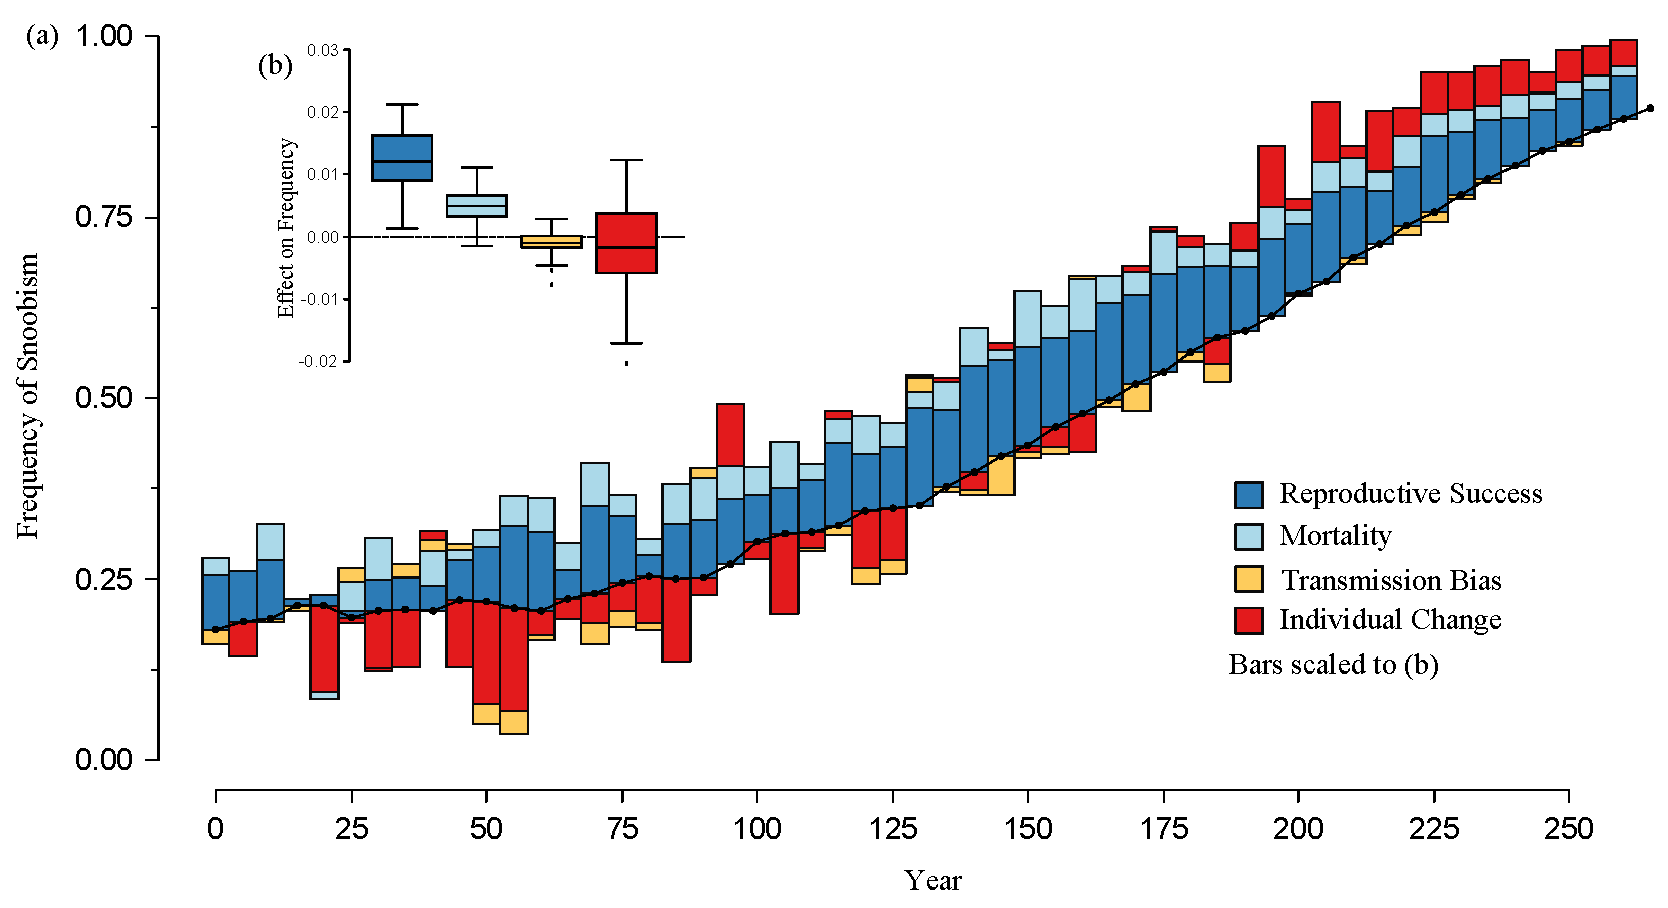
\includegraphics[scale=0.5]{figures/rtdice/FigSnoobCol.pdf}
\caption{(a) The population frequency of a binary cultural trait, Snoobism, observed over time, superimposed with the nonzero decomposition terms from the RTDICE equation.  Bars stacked above the Snoob frequency line represent positive magnitudes, and stacked below it, negative.  Since each bar represents one of the terms of Equation \ref{eq:RTDICE} (divided by $G$), their sum steers the direction of the frequency line.  For clarity, the bars are exaggerated to the scale in (b), which shows means, 5th, 25th, 75th and 95th percentiles of the observed annual decomposition magnitudes for each term.}
\label{fig:Snoob}
\end{center}
\end{figure}

Displaying each of the RTDICE magnitudes and directions graphically over time (Figure 1a) and in summary (Figure 1b) tells us immediately which of the decomposition terms played the largest role in driving the observed cultural trend.  For nearly three centuries, RS and mortality have consistently positive demographic effects on Snoobism, while parent-offspring transmission bias is small and apparently nondirectional.  Note that from the RTDICE decomposition itself we cannot tell if this RS effect results from differences in birth spacing, length of reproductive career, success in acquiring mates, or some combination of these.  Whatever the case, though, it is clear that on average Snoobs have more children than non-Snoobs, and that this is the most important trend in the evolution of Snoobism in the population over time.  

The strong, consistently positive effects from RS and mortality are not obvious from the frequency line itself, which for a full century shows little change in the prevalence of Snoobism in the population.  The decomposition terms indicate the reason: despite the fact the average Snoob has more children and is less likely to die than a non-Snoob, many more individuals abandon Snoobism than adopt it, maintaining Snoob frequency at around 20-25\%.  Only once this effect begins to vanish, 100 years after the settlement's founding, does Snoobism increase in frequency, and the last 15 census records all indicate a positive conversion balance that rivals the RS and mortality effects and facilitates Snoobism's eventual dominance.  

As with differential fertility and mortality, this reversal is consistent with many hypotheses. For example, it could be that an environmental or social change occurred some time between the years 130 and 180, after which Snoobism appeared to be an inherently more attractive lifestyle. Perhaps Snoobs developed a new institution for promoting conversion or preventing apostasy, or became politically dominant over non-Snoobs.  The trend is also consistent with a social learning hypothesis. Suppose, for example, that individuals tend to conform to the beliefs of the majority; then we would expect the conversion balance to covary with $\overline{\phi}$.  In our view, evolutionary decomposition is most valuable because such revealed trends can motivate targeted statistical modeling, which in turn can make predictions about future change.  

From the decomposition figures, we can also clearly see which processes \textit{don't} have large impact on the evolutionary trajectory. If we were measuring traits that are mostly transmitted horizontally within cohorts, such as musical preferences or use of a new technology, we expect to see a large transmission bias between parents and children.  This will also occur when measuring a life history characteristic like body weight or hunting skill, and as we discuss later this may even motivate a more sophisticated decomposition equation. The small bars of the transmission bias term in Figure 1 show that this is not true for one's Snoob status - children, when first censused, reliably hold the traits of their parents, Snoob or non-Snoob.

It should be noted that the apparent lack of a strong transmission bias does not render the process of character transmission unimportant. The fact that offspring tend to resemble their parents on average suggests that the Snoob trait is somehow heritable, and this heritability allows differential fertility and survival to affect the population mean. Still, Figure \ref{fig:Snoob} clearly shows that transmission bias in and of itself appears to have little direct effect on the rise of Snoobism, while the mechanisms behind RS, mortality and individual change all play determining roles.  


\section{Comparing Mechanisms of Cultural Change}

With decomposed trends now available, researchers can make informed forecasts about future change, compare parallel trends for other traits or in other populations, or design more specific goals for new rounds of data collection.  The most useful next step, in our opinion, is generating hypotheses about why these decomposition terms appear as they do, and developing and testing models of the mechanisms underlying these patterns.

For demonstration, we will focus here on the individual change term, with similar analyses of RS and mortality in the chapter appendix.  Among those individuals who appear in multiple censuses, we wish to know what effectively predicts their Snoob status, 0 or 1, at time $t+1$ given the information available at time $t$.  If we consider an individual $i$'s Snoob status in the next census, $\phi_{i,t+1}$, as a binomial random variable, possible mechanisms can be formalized as  conditional probabilities of becoming a Snoob.  To be precise, we will assume individuals retain their current Snoob status with probability $(1-L)$ and update with probability $L$, and using some learning rule $M$.  Then each model takes the form $\Pr(\phi_{i,t+1}=1) = LM + (1-L)\phi_{i,t}$.  As discussed above, the three-century-long swing in direction of the individual change term seems to point to several different, mutually-inclusive mechanisms: 

\textit{Conformist social learning.}  Under this mechanism, individuals tend to abandon Snoobism when it is unpopular, but become Snoobs when it is common.  Beginning with Boyd and Richerson's 1985 model, the conformist learning bias can be expressed in the form $M = \overline{\phi}_t + 2(\beta-1)(2\overline{\phi}_t - 1)\overline{\phi}_t(1-\overline{\phi}_t)$. Parameter $\beta$ represents the strength of conformity; when it is 1, updating is frequency-dependent but unbiased, and when it is greater than 1, updating is biased towards conformity.  More general, but more complicated, versions of this equation have been developed, allowing the conformity threshold to vary from a simple majority \citep{bowles2006microeconomics} and the strength of conformity to vary without bound \citep{mcelreath2008beyond}. 
 
\textit{Individual learning/density dependence.}  As the population is steadily growing in the simulator, the observed swing in the individual change term is also consistent with a simple density-dependence.  Under such a mechanism, the probability of becoming or remaining a Snoob increases with the island's population size, perhaps because non-confrontational Snoob norms are more attractive in crowded environments.  Thus, for population size $N_t$, the updating model may be written as $M=\mathrm{logit}^{-1}(\alpha + \beta N_t)$.  

\textit{Individual learning/environmental change.}  It is also plausible that individuals adopt or maintain Snoobism purely as a consequence of ``environmental'' decision-making, regardless of current population size or Snoob prevalence. Shocks due to technological ratcheting or climatological shifts may make Snoobism, with its thrifty norms and informal channels of social support, a more appealing lifestyle.  The observed swing in the individual change term, then, may be consequent from a changing material environment alone.  Absent any form of economic or ecological data, we can still model this using simple time series models, e.g. $M=\mathrm{logit}^{-1}(\alpha + \beta t)$, which can account for unobserved environmental shifts. 

Of course, in real populations such processes are probably all in effect to varying degrees, so more complex updating models that incorporate mixtures of these simple mechanisms should be included as well.  Using information-theoretic model comparison techniques, we fit a variety of such models, simple and complex, to the individual-level phenotypic data using maximum likelihood, and compared them using the Akaike Information Criterion and Schwartz Criterion (also called BIC).  Table \ref{tab:Learning} shows the four best-performing models, all conformist learning models.  The dominance of such models is most consistent with a pure conformist social learning hypothesis, at least among the few hypotheses tested above.\footnote{Unsurprisingly, this was the learning model used by the agents in \texttt{SnoobSim}.}  The two other major drivers of Snoobism, RS and mortality, were analyzed in a similar fashion in the chapter appendix.  Motivated by patterns in the decomposition terms, hypotheses about driving mechanisms of cultural evolution can be drawn from the rich theoretical literature and, using these methods, fitted to realistic field data.

\begin{table}[htbp]
  \centering
    \begin{footnotesize}
    \begin{tabular}{lccc}
    Updating Model, $M$ & Conformity Coefficient & AIC$_c$ Weight & BIC Weight \\
\hline
\hline
    $\overline{\phi}_t + 2(\beta-1)(2\overline{\phi}_t - 1)\overline{\phi}_t(1-\overline{\phi}_t)$ & 1.366 (1.322, 1.409) & 0.4049 & 0.5010 \\
    $\overline{\phi}_t^{\beta} / (\overline{\phi}_t^{\beta} + (1-\overline{\phi}_t)^{\beta})$ & 1.374 (1.318, 1.429) & 0.4019 & 0.4972 \\
    $\overline{\phi}_t + 2(\beta-1)(2\overline{\phi}_t - 2k)\overline{\phi}_t(1-\overline{\phi}_t)$ & 1.360 (1.311, 1.408) & 0.1743 & 0.0017 \\
    $\mathrm{logit}^{-1}(\alpha + \beta \overline{\phi}_t)$ & 6.389 (6.121, 6.658) & 0.0106 & 0.0001 \\
    \hline
    \end{tabular}%
    \caption{Top four models among the thirteen fitted to the simulated census data, as measured by AIC$_c$ and BIC score (see chapter appendix for full model list).  Each model $M$ of the thirteen is embedded in the equation $p=L(M) + (1-L)(\phi_{i,t})$, where $p$ describes the conditional probability an individual will be a Snoob in the next census, per $\phi_{i, t+1} \sim \mathrm{Binomial}(1, p)$.  The top four are all social learning models, each with a conformity coefficient $\beta$ of comparable meaning.  The first model above comes from Boyd and Richerson (1985), while the second and third come from McElreath, et al. (2008) and Bowles (2004), respectively.} 
		\label{tab:Learning}
    \end{footnotesize}

\end{table}

\newpage
\section{Discussion}

It is important to emphasize what the preceding evolutionary decomposition analysis gives us compared to standard demographic metrics. Birth and death rates could be more precisely compared using the total fertility rate, life expectancy at birth, or other common demographic measures. But by themselves these tools lack a direct mathematical connection to change in mean phenotype in the population, the most common way we measure evolution.  As a result, it is difficult to assess exactly how much mortality affects the population distribution of phenotype, versus RS, immigration, and so forth.  

These answers are readily available from decomposition of mean phenotypic change, regardless of the particularities of the system.  Phenotypes may be discrete values like Snoob status, or continuous, like body weight.  Because the decomposition equation is derived from basic facts about the population and data structure, its value depends not in the realism of its assumptions (which we contend are nearer to axioms), but rather in the meanings we can find in its terms, once strictly defined.  In doing so, three important qualifications must be stressed. 

First, the terms in the decomposition equation segregate but do not correspond exactly to evolutionary processes like sexual selection or biased social learning.  Snoobs may enjoy higher RS because of something inherent in practicing Snoobism, because the trait co-occurs with some other trait like income or age, or simply due to chance. The decomposition terms, most of which are covariances between phenotype and demographic outcomes, are really nothing more that dimensionalized correlations.  Following Rice \citeyearpar{rice2004evolutionary} and Henrich et al. \citeyearpar{Henrich2008:misunderstandings}, we feel that terms like ``selection'' or ``fitness'' should only be invoked when a \textit{causal} pathway between phenotype and outcome can be supported, and even then any empirical decomposition term will be a combination of both causal and noncausal associations. 

Second, the RTDICE decomposition is only one possible partitioning of the observed phenotypic trajectory, and potentially not a very useful one.  For example, the differential mortality between Snoobs and non-Snoobs is partially a consequence of the fact Snoobs tend to be younger, which is a consequence of their differential RS.  We can use logistic models of mortality to establish that Snoob status predicts mortality outcomes even among those of the same age (see chapter appendix), but the RTDICE mortality term cannot isolate this effect from the covariance between Snoobism and age.  If we expect structuring variables like age, gender, ethnic group, or location in a metapopulation will play an important role in the evolution of a particular phenotypic character, we should build this directly into the decomposition equation as appropriate for the dataset and the situation \citep{coulson2008dynamics}.  

We must also modify the equation if the categories we place people within are inappropriate, e.g. the intercensus period spans multiple generations, parentage cannot be identified, or we wish to distinguish immigrants from different sources.  Note that we need no special consideration of whether the parent of record is a genetic parent, and if appropriate we may specify other inheritance relationships like ``teacher'' or ``older sibling''; the evolutionary consequences of the observed relationship are an empirical matter.

The third qualification is that, without records of each demographic event as it happened, the terms in a decomposition equation should not be viewed as strictly independent.  The effects of intercensus events are inferred from comparing the two census records, but some information is necessarily lost, such as individual change shortly before death or after birth. 

In fact, if the population experiences demographic events in discrete seasons, the terms can lose their distinctiveness altogether.  Imagine, for example, a population of individuals experience heavy mortality in each winter, selecting out individuals with smaller phenotypes (e.g. weight, beak length).  Then, in the summer, the survivors give birth.  Applying RTDICE to annual census records would show a strong covariance between RS and phenotype even if phenotype plays no important role in mating or reproducing, simply because of the preceeding mortality event.  

We suspect that for large populations in which such demographic events do not follow a strict order, the distortions are minimal.  We can never properly rid ourselves of the problem of order, however, since every death removes the possibility of another birth, emigration event, etc.  For populations which do go through a distinct schedule of demographic events, one possible solution is to construct ordered-event decomposition equations.  

As in Coulson and Tuljapurkar \citeyearpar{coulson2008dynamics}, the RTDICE equation only holds exactly for full census data without error. We realize that probably no dataset of the size and quality comparable to that simulated here exists in reality; real datasets nearly always contain just a sample of the full population and some amount of measurement error. Under circumstances of incomplete data, the terms of the RTDICE equation cannot simply be computed but must instead be estimated by statistical analysis. We anticipate that future research will elucidate the best statistical methods for estimating these terms.

Despite these limitations, we foresee a wide variety of applications for the decomposition approach in both evolutionary theory and studying human history.  The decomposition method provides unique advantages in profiling trends, motivating and testing hypotheses, and assisting prediction.  By applying basic demographic bookkeeping to high-resolution records of cultural change over time, we are also able to demonstrate conclusively the Darwinian nature of cultural transmission.    





\section{Appendix to Chapter 2}

All models below were coded in R using variables extracted from the 54 SnoobSim census records.  Models were fit by maximum likelihood using the function \texttt{mle2} in Ben Bolker's \texttt{bbmle} package (cran.r-project.org/), with the default BFGS algorithm.

\subsection{Extended Analysis of Individual Change}

The ``individual change'' decomposition bars indicate that initially the balance of change is negative and large in magnitude.  As the frequency of Snoobs approaches 50\%, though, this effect becomes smaller and smaller, and as Snoobs move towards fixation the effect reverses and the balance of converts is now strongly positive, at times rivaling RS in magnitude.

An important thing to keep in mind when reading the individual change bars is that they represent only the average phenotypic cange across individuals; some individuals became Snoobs in the first few decades, but more apostatised to non-Snoob.  

Our outcome variable here is ``will be a Snoob'' in the next census ($\phi_{i,t+1}$), modeled by current Snoob status and other properties of individuals and the population.  Because we have a binary outcome variable, we use a binomial model with various parameterizations of $p$.  A standard way to express this probability is the form $p = LM + (1-L)\phi_{i,t}$, so individuals update with probability $L$ and retain their current status with probability $(1-L)$.  Strictly speaking, this sequence of first updating, then (potentially) changing phenotype implied by this model is quite artificial for real human learning.  However, it is interesting to consider human cultural change \textit{as if} it proceeded in this fashion, because the updating rule can incorporate a variety of hypothesized mechanisms for comparison using information criteria. 

The simplest model is a constant Snoob conversion probability for all individuals
	\[M_0 = \alpha.
\]
In other words, individuals update with probability $L$, and of those we expect fraction $\alpha$ take Snoobism as their phenotype.

Conformist learning is parameterized in four, very similar, ways.  The model $\overline{\phi}_t + D(2\overline{\phi}_t-1) \overline{\phi}_t (1-\overline{\phi}_t)$ is from \cite{boyd1985culture}.  Parameter $D$ represents the strength of conformity; $D=0$ indicates no conformity and unbiased, frequency-dependent learning.  If $D > 0$, conformity will increasingly dominate the probability of becoming a Snoob, while $D < 0$ implies non-conformity (you are more likely to choose the opposite of the majority's trait).  Bowles \cite{bowles2006microeconomics} modifies this by creating an explicit parameter for the threshold, allowing it to vary from 0.5, so which we could write as $\overline{\phi}_t + D(2\overline{\phi}_t-2k)\overline{\phi}_t(1-\overline{\phi}_t)$.  The conformity model in McElreath, et al. \citep{mcelreath2008beyond}\footnote{The basic form of this model was suggested to McElreath et al. by Sam Bowles (Richard McElreath, \textit{personal communication}).} expresses a similar idea, using the model
	\[ M_1 = \frac{\overline{\phi}_t^\beta}{\overline{\phi}_t^\beta + (1-\overline{\phi}_t)^\beta}
\]
where $\beta > 1$ represents conformity.  Because the Boyd and Richerson model is actually Taylor series approximation of this more general model when $\beta$ is close to 1 and $\overline{\phi}_t$ is near 0.5, we may sensibly write all three models in a common notation.  Hence, in our analysis, we include the 1985 model as
	\[ M_2 = \overline{\phi}_t + 2(\beta-1)(2\overline{\phi}_t-1),
\]
and the 2004 model as
	\[ M_3 = \overline{\phi}_t + 2(\beta-1)(2\overline{\phi}_t-2k).
\]
Another sensible way to parameterize conformity is by using a logit link function, such that
	\[ M_4 = \mathrm{logit}^{-1}(\alpha + \beta \overline{\phi}_t) = \frac{\exp(\alpha + \beta \overline{\phi}_t)}{1 + \exp(\alpha + \beta \overline{\phi}_t)}. \]

Two density-dependent models, one with a quadratic effect,
	\[ M_5 = \mathrm{logit}^{-1}(\alpha + \beta N_t),\]
	\[ M_6 = \mathrm{logit}^{-1}(\alpha + \beta_1 N_t + \beta_2 N_t^2).\]
Model $M_6$ used population sizes coded in standard units, to aid the maximum likelihood algorithm. Two time series models, one with a quadratic effect,
	\[ M_7 = \mathrm{logit}^{-1}(\alpha + \beta t),\]
	\[ M_8 = \mathrm{logit}^{-1}(\alpha + \beta_1 t + \beta_2 t^2 ).\]
Oscillatory models of time and population were also used:
	\[ M_9 = \mathrm{logit}^{-1}(\alpha + \beta_1 \sin (\beta_2 t)),\]
	\[ M_{10} = \mathrm{logit}^{-1}(\alpha + \beta_1 \sin (\beta_2 N_t)).\]
Various combinations were also included.  Including time and population size,
\[ M_{11} = \mathrm{logit}^{-1}(\alpha + \beta_1 t + \beta_2 N_t).\]
Including population Snoob frequency, individual age in years (centered on mean), and gender (coded as a 1/0 variable ``male''),
\[ M_{12} = \mathrm{logit}^{-1}(\alpha + \beta_1 \overline{\phi}_t + \beta_2 \mathrm{male} + \beta_3 \mathrm{age}).\]
The final model included adds time to model $M_{12}$,
\[ M_{13} = \mathrm{logit}^{-1}(\alpha + \beta_1 \overline{\phi}_t + \beta_2 \mathrm{male} + \beta_3 \mathrm{age} + \beta_4 t).\]
Running a model comparison ranks these thirteen models according to Table \ref{tab:ichangemodels}.  Schwartz criterion ranks (BIC) are nearly identical to AIC$_c$ ranks, nominating models $M_1$ and $M_2$ as the best-performing.  The constant model, $M_0$, performs worst among the model set, but conformity models completely dominate the model weighting.  This would indicate that the best out-of-sample predictive models as identified by information theory are purely social learning models using $\overline{\phi}_t$, and do not improve by adding other population-level covariates like population size, or individual-level variables like gender or age.

 
\begin{table}[htbp]
  \centering
    \begin{tabular}{lrrrrr}
  	\hline
  	\hline
    Model & $k$ & AIC$_c$ weight & BIC weight & $\Delta$ AIC$_c$ & $\Delta$ BIC \\
   	\hline
    $M_2$  & 2     & 40.49\% & 50.10\% & $<$0.01  & $<$0.01 \\
    $M_1$  & 2     & 40.19\% & 49.72\% & 0.02  & 0.02 \\
    $M_3$  & 3     & 17.44\% & 0.17\% & 1.69  & 11.42 \\
    $M_4$  & 3     & 1.06\% & 0.01\% & 7.28  & 17.02 \\
    $M_{12}$ & 5     & 0.58\% & $<$0.01\% & 8.48  & 37.68 \\
    $M_{13}$ & 6     & 0.24\% & $<$0.01\% & 10.27 & 49.21 \\
    $M_6$  & 4     & $<$0.01\% & $<$0.01\% & 67.35 & 86.82 \\
    $M_8$  & 4     & $<$0.01\% & $<$0.01\% & 102.91 & 122.38 \\
    $M_7$  & 3     & $<$0.01\% & $<$0.01\% & 107.40 & 117.14 \\
    $M_5$  & 3     & $<$0.01\% & $<$0.01\% & 921.84 & 931.57 \\
    $M_{11}$ & 4     & $<$0.01\% & $<$0.01\% & 1070.58 & 1090.05 \\
    $M_{10}$ & 4     & $<$0.01\% & $<$0.01\% & 2007.97 & 2027.44 \\
    $M_9$  & 4     & $<$0.01\% & $<$0.01\% & 2254.17 & 2273.64 \\
    $M_0$  & 1     & $<$0.01\% & $<$0.01\% & 133107.95 & 133098.21 \\
    \hline
    \end{tabular}%
    \caption{Individual change updating models, by AIC$_c$ rank, with AIC$_c$ and BIC scores in terms of the top model, $M_2$, and model weights (all to two decimal places).  Both the Akaike Information Criterion and the Schwartz Criterion (BIC) rank the performance of each model by assigning penalties to its MLE likelihood value; AIC and AIC$_c$ penalize by the number of parameters, $k$, in a given model.}
  \label{tab:ichangemodels}%
\end{table}%

Because of the functional similarity between $M_1$, $M_2$, and $M_3$, the parameter estimates are nearly identical, and only $M_1$ will be discussed.  The conformity coefficient (with standard error) was estimated as 1.374 (0.028), which, being above 1, is evidence towards conformist biased updating.  The maximum-likelihood estimate for the intercensus updating probability, $L$, was 0.100 (0.002), meaning that under this model about 10\% of the population updates every five years, while 90\% do not update at all.  It is worth noting these estimates are quite sensible per what the SnoobSim software is actually doing (next section).

\begin{figure}[t]
\begin{center}
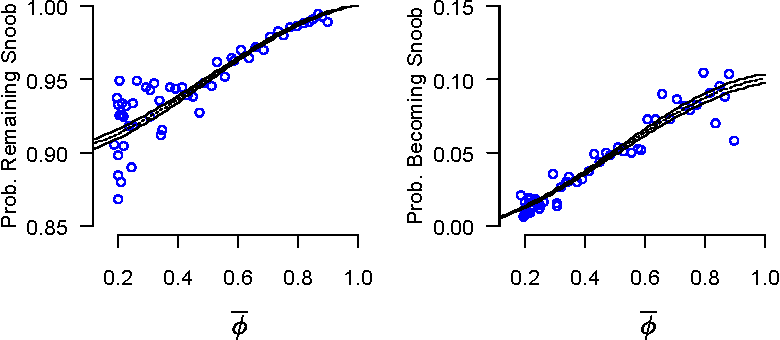
\includegraphics[scale=1]{figures/rtdice/ichange.pdf}
\caption{Fitted model $M_1$ plotted over the observed proportions of individuals who will switch to or remain Snoobs intercensus, on the population Snoob frequency for the first 53 censuses.  Maximum likelihood estimates (dashed line) and 95\% HPDI intervals (solid lines) for the Bernoulli probability of becoming a Snoob, $p$, show a strong nonlinear association between individual change and $\overline{\phi}_t$.}
\label{fig:ichange}
\end{center}
\end{figure}


\subsubsection{Individual Change - What SnoobSim is Actually Doing}

In the simulation, each day, some fraction of the population decides they will ``update'' their Snoob status.  To be precise, each individual updates daily with probability 0.00006.  If an individual decides to update, they then collect a random sample of 100 people in the population, and uses this information to decide to change their Snoob status or stay where they are.  Note that once an individual decides to update, their previous Snoob status becomes irrelevant.  Each individual takes their particular sample of 100 and adopts Snoobism with probability given by the code:

\begin{verbatim}
prob.converting.to.snoob <- 
	(sample.frq^conformity.bias.snoob)/
	(sample.frq^conformity.bias.snoob	+ (1-sample.frq)^conformity.bias.snoob)
\end{verbatim}

In other words, learners used exactly the same mechanism as $M_1$, except on the Snoob frequency among the 100 they randomly sampled, rather than the population frequency.  No surprise, then, that models with this functional form came in first in the model comparison.  The simulation parameter \texttt{conformity.bias.snoob} was set to 1.3 (compare against the MLE of $\beta$ above), and with a daily probability of updating set to 0.00006, we expect proportion $1-(1-0.00006)^{365\times5}=0.104$ of the population to update (compare to the MLE of $L$, above).  We should not expect real census data to nominate such simple models, but the utility of information-theoretic model comparison remains the same nonetheless.


\subsection{Analysis of RS Term}

The strong, consistently positive effect of RS in the decomposition indicates that Snoobs have more children than non-Snoobs, on the average.  This could be causal, meaning Snoobism itself may have some effect on one's desire or ability to mate, or it could be a consequence of Snoobism covarying with some other trait.  For example, if people tend to become Snoobs during their reproductive careers, only to abandon it later in life, we would see a consistent, positive effect in the decomposition.  Or, perhaps Snoobism is a sex-specific trait and there are fewer of that gender in the population (so they must have higher mean RS).  

Hence, it is premature to say Snoobism is ``under selection'' without conclusive evidence against confounding variables.  This is difficult to impossible in observational contexts, like this one, but statistical control can at least tell us if the RS advantage of Snoobs remains when comparing Snoobs and non-Snoobs of the same gender and age.  

Our outcome variable is the number of kids an individual sires (if they are of reproductive age) have during the next intercensus period, which in our data varies between 0 and 8 (women are constrained to about 5 or 6 children in a five-year intercensus period), $f_{i, t+1}$.  We have some flexibility with count data, so we have chosen to compare models of the outcome variable using three possible probability distributions: geometric, Poisson, and zero-inflated Poisson.  For the Poisson family, $\lambda$ is modeled by an exponential link function ($\lambda = \exp(M)$, for some model $M$), while for the geometric models, the Bernoulli probability of success $p$ is modeled generically by logit link function ($p=\mathrm{logit}^{-1}(M)$).  

Altogether, twelve models of the expected number of intercensus children were compared.  Note that all uses of age center the variable on its mean.
	\[M_0 = \beta_0
\]
	\[M_1 = \beta_0 + \beta_1 \mathrm{age}
\]
	\[M_2 = \beta_0 + \beta_1 \mathrm{age} + \beta_2 \mathrm{(age)}^2
\]
	\[M_3 = \beta_0 + \beta_1 \mathrm{age} + \beta_2 \mathrm{(age)}^2 + \beta_3 \phi_{i,t}
\]
	\[M_4 = \beta_0 + \beta_1 \mathrm{age} + \beta_2 \mathrm{(age)}^2 + \beta_3 \phi_{i,t} + \beta_4 \mathrm{male}
\]
	\[M_5 = (1-N_t/K)(\beta_0 + \beta_1 \mathrm{age} + \beta_2 \mathrm{(age)}^2 + \beta_3 \phi_{i,t} + \beta_4 \mathrm{male})
\]
	\[M_6 = \exp(-K*N_t)(\beta_0 + \beta_1 \mathrm{age} + \beta_2 \mathrm{(age)}^2 + \beta_3 \phi_{i,t} + \beta_4 \mathrm{male})
\]
	\[M_7 = \beta_0 + \beta_1 \mathrm{age} + \beta_2 \overline{\phi}_t
\]
	\[M_8 = \beta_0 + \beta_1 \mathrm{age} + \beta_2 \mathrm{(age)}^2 + \beta_3 \overline{\phi}_t
\]
	\[M_9 = \beta_0 + \beta_1 \mathrm{age} + \beta_2 \mathrm{(age)}^2 + \beta_3 \phi_{i,t} + \beta_4 \overline{\phi}_t
\]
	\[M_{10} = \beta_0 + \beta_1 \mathrm{age} + \beta_2 \mathrm{(age)}^2 + \beta_3 \phi_{i,t} + \beta_4 \mathrm{male} + \beta_5 \overline{\phi}_t
\]
	\[M_{11} = \beta_0 + \beta_1 \mathrm{age} + \beta_2 \mathrm{(age)}^2 + \beta_3 \phi_{i,t} + \beta_4 \mathrm{male} + \beta_5 (\mathrm{male} \times \phi_{i,t})
\]
	\[M_{12} = \beta_0 + \beta_1 \mathrm{age} + \beta_2 \mathrm{(age)}^2 + \beta_3 \phi_{i,t} + \beta_4 \mathrm{male} + \beta_5 \overline{\phi}_t + \beta_6 (\mathrm{male} \times \phi_{i,t})
\]
Since each of these 12 models can be placed within a Poisson, geometric, or zero-inflated Poisson (ZIP) distribution, a total of 36 distinct models are fitted separately to the data and compared for out-of-sample predictive accuracy using AIC$_c$ and BIC (Table \ref{tab:RScompare}).

The top models, $M_{10}$ and $M_{12}$, both include age, gender and Snoob status, and differ only in an interaction effect between male and Snoob status.  No density-dependent or frequency-dependent models performed as well.  Also, according to the model comparison, the zero-inflated Poisson distribution is the best-performing stochastic wrapper around these two models, as opposed to the geometric distribution or the Poisson, which are vastly outperformed.

Estimates and confidence intervals for $M_{10}$ are presented in table \ref{tab:m10ests}, with MLE-fitted lines plotted in Figure \ref{fig:rs}.  It is clear from the estimates and figure that Snoobism remains an excellent predictor of reproductive output after accounting for age and gender.  This allows us to rule out the possibility that the decomposition results for RS were merely a consequence of chance associations between Snoobism and age or gender, and points to the possibility Snoobism is under some form of fecundity or sexual selection.    

\begin{table}[htbp]
  \centering
    \begin{tabular}{lcrrrr}
    \hline
    \hline
    Parameter & Estimate & Std. Error & 2.50\% & 97.50\% \\
    \hline
    $\beta_0$    & -0.878 & 0.024 & -0.924 & -0.831 \\
    $\beta_1$    & -0.006 & $<$0.001 & -0.007 & -0.005 \\
    $\beta_2$    & -0.002 & $<$0.001 & -0.003 & -0.002 \\
    $\beta_3$    & 0.681 & 0.017 & 0.647 & 0.714 \\
    $\beta_4$    & 0.120 & 0.013 & 0.093 & 0.147 \\
    $\beta_5$    & 0.244 & 0.033 & 0.179 & 0.309 \\
    $\alpha$ & 0.357 & 0.006 & 0.3451 & 0.369 \\
    \hline
    \end{tabular}%
    \caption{Parameter estimates for the zero-inflated Poisson version of model $M_{10}$.  The second-placed model's fitted values are nearly identical to these but with an additional interaction term for Male snoobs of -0.043 (0.030), MLE and SE.  Parameter $\alpha$ estimates the frequency an outcome of 0 will be drawn from the distribution, beyond what would be expected by the Poisson model.} 
  \label{tab:m10ests}%
\end{table}%

\begin{table}[htbp]
  \centering
    \begin{tabular}{llrrrrr}
    \hline
    \hline
    Model & Distribution & $k$ & AIC$_c$ weight & BIC weight & $\Delta$ AIC$_c$ & $\Delta$ BIC \\
    \hline
    $M_{10}$ & ZIP   & 7     & 72.35\% & 99.63\% & 0.00  & 0.00 \\
    $M_{12}$ & ZIP   & 8     & 27.65\% & 0.37\% & 1.92  & 11.17 \\
    $M_{12}$ & Geom. & 7     & 0.00\% & 0.00\% & 28.19 & 28.19 \\
    $M_{10}$ & Geom. & 6     & 0.00\% & 0.00\% & 36.98 & 27.73 \\
    $M_4$  & ZIP   & 6     & 0.00\% & 0.00\% & 52.23 & 42.98 \\
    $M_{11}$ & ZIP   & 7     & 0.00\% & 0.00\% & 53.70 & 53.70 \\
    $M_{11}$ & Geom. & 6     & 0.00\% & 0.00\% & 72.55 & 63.30 \\
    $M_{4}$ & Geom. & 5     & 0.00\% & 0.00\% & 80.50 & 62.00 \\
    $M_3$  & Geom. & 4     & 0.00\% & 0.00\% & 98.63 & 70.87 \\
    $M_3$  & ZIP   & 5     & 0.00\% & 0.00\% & 129.07 & 110.57 \\
    $M_8$  & Geom. & 4     & 0.00\% & 0.00\% & 1553.27 & 1525.52 \\
    $M_8$  & ZIP   & 5     & 0.00\% & 0.00\% & 1699.65 & 1681.15 \\
    $M_{12}$ & Poisson & 7     & 0.00\% & 0.00\% & 1779.76 & 1779.76 \\
    $M_{10}$ & Poisson & 6     & 0.00\% & 0.00\% & 1795.46 & 1786.21 \\
    \hline
    \end{tabular}%
    \caption{Models of reproductive success, by AIC$_c$ and BIC rankings to two decimal places.  Models can appear more than once in the rankings because they are embedded in different stochastic nodes: the second-ranked model is $M_{12}$ in a zero-inflated Poisson distribution (ZIP), while the third-ranked model is $M_{12}$ in a geometric distribution.  Of the 36 models tested (three stochastic distributions for each of twelve structural models), only the top 14 are shown.}
  \label{tab:RScompare}%
\end{table}%


\begin{figure}[t]
\begin{center}
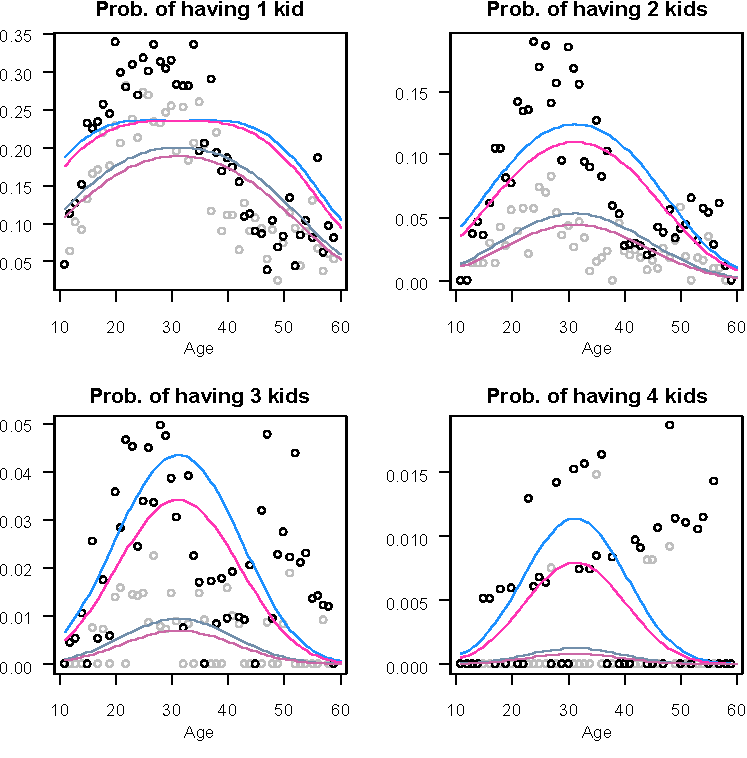
\includegraphics[scale=1]{figures/rtdice/rs.pdf}
\caption{Fitted model $M_{10}$ plotted over the observed proportions of parents with exactly a certain number of intercensus children, by parent age.  For each of the 53 intercensus periods, Snoobs (black circles) have more children on average than non-Snoobs (gray circles), which reflected by the fitted lines as well.  Snoob men (bright blue) have more children on average than both Snoob women (bright pink) and non-Snoob men (dark blue), implying a sex-ratio imbalance.}
\label{fig:rs}
\end{center}
\end{figure}


\subsubsection{Reproductive Success: What SnoobSim is Actually Doing}

Women become pregnant probabilistically according to an age-specific fertility schedule identical to that of a realistic population (US women c. 2005).  From the ages of 15 to 50, women reference a daily probability of conception given by

\begin{verbatim}
daily.pr.conception <- (1-(1/(1+exp(alpha + beta1*snoob))))
\end{verbatim}

Parameter \texttt{alpha} is set by the fertility schedule, and the effect of being a Snoob is for this run is \texttt{beta1}=0.8, exaggerating a Snoob's age-specific fertility schedule and increasing the daily probability she will become pregnant.  If a woman conceives, she will then choose a male as the father.  

Men are promiscuous and can be chosen by multiple women (one lucky man fathered a record 8 kids in 5 years with several different women).  Women will continue to mate with the same man until he becomes unavailable due to advanced age (i.e. greater than 60 years old) or death.

According to the simulator parameters, women almost always choose males who are like them with respect to Snoob status.  Men enjoy no specific fertility schedule, but because of this positive assortment we can expect Snoob men will have different fertility schedules than nonSnoob men.  However, a man's age (or any other traits for that matter) has nothing to do with his being selected, so we should not expect a male's age-specific fertility to be like a female's.  Nevertheless, mechanistically Snoobism has a direct impact on one's RS, and this effect cannot be controlled out by including other covariates.  As far as the simulation is concerned, Snoobism is indeed under strong fertility selection.


\subsection{Analysis of Mortality Term}

According to the RTDICE decomposition, non-Snoobs die more than Snoobs, causing Snoobism to consistently increase by a relatively small amount.  As with positive RS, this could be a result of a behavior consequent from Snoobism itself, in which case we could say the positive mortality effect is ``viability selection''.  But, alternatively, this effect could be due to an association between Snoobism and some other trait which confers differential survival.  For example, if young people are more attracted to Snoobism, while seniors tend to dismiss it as a folly of youth, Snoobism would negatively covary with mortality despite having no mechanistic effect on one's mortality.
                            
Our goal, then, is to establish whether Snoob status still helps predict mortality outcomes even after accounting for age, gender, and other relevant life history characteristics.  This motivates a number of mortality models.  Because we can work with individual-level data for multiple time periods, we specifically wish to model whether in the next intercensus period an individual will die ($d_{i,t+1} = 1$) or not ($d_{i,t+1}=0$), using their gender, age, and Snoob status, and possibly properties of the population.  This outcome is modeled as a binomial random variable, or $d_{i,t+1} \sim \mathrm{Binomial}(1,p)$, with $p$ taking the form of an inverse logit link of some model $M$.

A total of six models were included in this analysis:
	\[M_0 = \alpha
\]
	\[M_1 = \alpha + \beta_1 \mathrm{age}
\]
	\[M_2 = \alpha + \beta_1 \mathrm{age} + \beta_2 \mathrm{(age)}^2
\]
	\[M_3 = \alpha + \beta_1 \mathrm{age} + \beta_2 \mathrm{(age)}^2 + \beta_3 \mathrm{male}
\]
	\[M_4 = \alpha + \beta_1 \mathrm{age} + \beta_2 \mathrm{(age)}^2 + \beta_3 \mathrm{male} + \beta_4 \phi_{i,t}
\]
	\[M_5 = \alpha + \beta_1 \mathrm{age} + \beta_2 \mathrm{(age)}^2 + \beta_3 \mathrm{male} + \beta_4 \phi_{i,t} + \beta_5 \overline{\phi}_t
\]
Because long-lived humans record many zeros for this variable until their eventual death, we also considered a zero-inflated binomial stochastic node with the same logit-linked models of $p$, for a total of 12 models.  Comparing these as before produces Table \ref{tab:morttab}, which shows one clear winner: $M_4$ for the binomial distribution.  In other words, the information criteria suggest that the best way to predict one's mortality status is by knowing their age, gender, Snoob status together.  Plotting this fitted model on proportions of individuals who die at particular ages produces Figure \ref{fig:mortality}.  The $M_4$ are not perfect, but correctly identify the different mortality experiences across the lifetime for Snoob and non-Snoob (Table \ref{tab:m4ests}).  As with RS, we can show clearly that Snoobism remains a useful predictor even accounting for age and gender, which may indicate that viability selection is in play in the mortality term in the decomposition.  



\begin{figure}[t]
\begin{center}
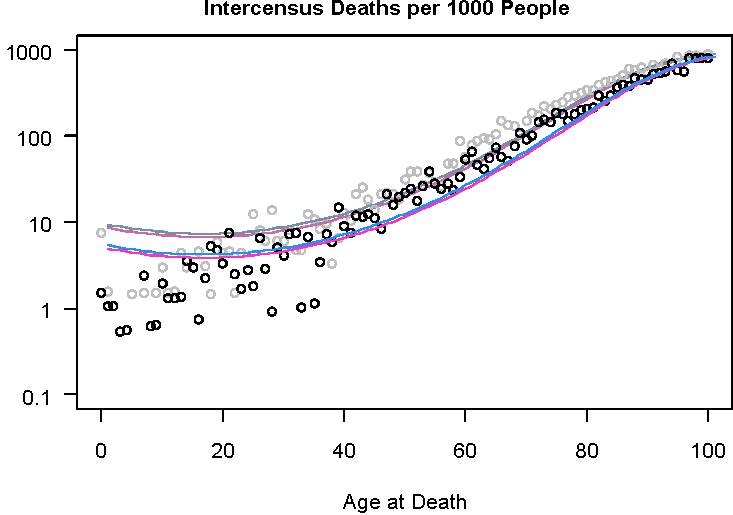
\includegraphics[scale=1]{figures/rtdice/mortality.pdf}
\caption{Fitted model $M_{4}$ plotted over the observed proportion of intercensus deaths per 1000 people by age.  For each of the 53 intercensus periods, Snoobs (black circles) die less frequently than non-Snoobs (gray circles), which reflected by the fitted lines as well.  Snoob women (bright pink) survive most frequently, closely followed by Snoob men (bright blue).  Non-Snoob men (dark blue) die most frequently of all, but at rates comparable to non-Snoob women (dark pink).}
\label{fig:mortality}
\end{center}
\end{figure}


% Table generated by Excel2LaTeX from sheet 'mort'
\begin{table}[htbp]
  \centering
  
    \begin{tabular}{llrrrrr}
    \hline
    \hline
    Model & Distribution & $k$     & AIC$_c$ weight & BIC weight & $\Delta$ AIC$_c$ & $\Delta$ BIC \\
    \hline
    $M_4$    & binomial & 5     & 100.00\% & 99.99\% & 0.00  & 0.00 \\
    $M_5$   & ZIB   & 7     & 0.00\% & 0.00\% & 20.41 & 39.87 \\
    $M_5$    & binomial & 6     & 0.00\% & 0.00\% & 21.20 & 30.94 \\
    $M_1$    & binomial & 2     & 0.00\% & 0.01\% & 47.62 & 18.41 \\
    $M_3$    & binomial & 4     & 0.00\% & 0.00\% & 49.82 & 40.08 \\
    $M_4$   & ZIB   & 6     & 0.00\% & 0.00\% & 76.98 & 86.71 \\
    $M_2$    & binomial & 3     & 0.00\% & 0.00\% & 122.52 & 103.05 \\
    $M_2$   & ZIB   & 4     & 0.00\% & 0.00\% & 309.24 & 299.50 \\
    $M_3$   & ZIB   & 5     & 0.00\% & 0.00\% & 717.33 & 717.33 \\
    $M_1$   & ZIB   & 3     & 0.00\% & 0.00\% & 1349.15 & 1329.68 \\
    $M_0$    & binomial & 1     & 0.00\% & 0.00\% & 15489.56 & 15450.62 \\
    $M_0$   & ZIB   & 2     & 0.00\% & 0.00\% & 15491.56 & 15462.36 \\
    \hline
    \end{tabular}%
    \caption{Model rankings for mortality models, with number of parameters ($k$).  To two decimal places, model $M_4$ completely dominates the information criterion weightings.}
  \label{tab:morttab}%
\end{table}%


\begin{table}[htbp]
  \centering
    \begin{tabular}{lcrrrr}
    \hline
    \hline
    Parameter & Estimate & Std. Error & 2.50\% & 97.50\% \\
    \hline
    $\alpha$    & 4.673 & 0.040 & 4.595 & 4.750 \\
    $\beta_1$    & -0.036 & 0.001 & -0.039 & -0.034 \\
    $\beta_2$    & -0.001 & 0.000 & -0.001 & -0.001 \\
    $\beta_3$    & -0.088 & 0.034 & -0.155 & -0.021 \\
    $\beta_4$    & 0.559 & 0.034 & 0.492 & 0.627 \\
    \hline
    \end{tabular}%
    \caption{Parameter estimates for model $M_{4}$ in a binomial model of mortality.  Snoob status substantially reduces the probability one will die at any given age or gender.} 
  \label{tab:m4ests}%
\end{table}%




\subsubsection{Mortality - What SnoobSim is Actually Doing}

Snoobs reference a different mortality schedule in the simulation specific to their age and gender.  The baseline mortality schedule for non-Snoobs is the estimated US mortality schedule c. 2005.  To be specific, the daily probability of death for each individual is calculated via:

\begin{verbatim}
daily.pr.death <- (1-(1/(1+exp(alpha + mortality.bias.male*male 
                                       + mortality.bias.snoob*snoob))))
\end{verbatim}

The parameter alpha represents the mortality schedule, but can be modified by both gender and Snoob status.  For this simulation, \texttt{mortality.bias.snoob} was set to -0.5, meaning Snoobs die less often, and and the \texttt{mortality.bias.male} was 0.3, meaning males die more often.  As a consequence, Snoobs should always die less for any given age and gender, and so the effects of this ``viability selection'' should show up in models that account for Snoob status.  



\subsection{SnoobSim Documentation}

SnoobSim is an agent-based population simulator in R that can be used to simulate virtually any demographic process in small populations.  It works by running through a daily list of stochastic events within the population and updating a master population register based on the outcome of these events, which can be influenced by the user.  Because population changes over decades, centuries, or longer can be simulated, a full record of every event inside the simulation is not intended to be saved.  Rather, the simulator records and exports census records taken in intervals specified by the researcher (e.g. every five years).  When it is time for another census, a copy of the population register for that day is saved, and when the simulation ends all such censuses are saved in csv format, as real field data would be stored.
  
Control of the simulator is managed through the ``control panel", a list of parameters at the top of the SnoobSim.r script.  These are divided into basic simulator values, such as the time between each census, initial population size, etc, vital population rates, such as age-specific fertility and mortality, etc. and evolutionary mechanisms, which control how the phenotypic traits of each individual are determined, and how they influence demographic parameters.  

Each day, the following demographic processes occur in this order:\\
1.	immigration \\
2.	births\\
3.	matings\\
4.	deaths\\
5.	emigration\\
6.	social learning / individual change\\

Since the simulation loops over days, which have relatively few births and deaths for realistic human populations, we expect that there are no important difficulties introduced by this order, or important differences if the order were changed.  

Immigration is controlled by two functions - \texttt{daily.immigration} and \\ \texttt{immigrant.maker}.  The first determines how many individuals will immigrate into the population that day, following the crude immigration rate specified by the user.  If there are indeed immigrants that day, the \texttt{immigrant.maker} function will create new entries in the population register for each of them. 

Mating occur only if there are fecund males and females.  Any female between 15 and 50 years old who is not currently pregnant can mate, as can any male between 15 and 60.  The \texttt{conception} function determines first if any women who can mate will actually do so that day; it determines this probabilistically by referencing an age-specific fertility schedule specified by the user.  Once it is determined that a female will become pregnant that day, the female will then choose an available male to be the father.  This is accomplished via the \texttt{mate.finder} function.  If no males are available then the woman will not become pregnant, but if at least one is available she will choose a male, each will count the other as their ``mate" in the population register, and the woman will become pregnant, beginning a daily countdown until birth saved to the ``counter" column in the population register.  The length of pregnancy here is approximately normal with mean 280 days and a standard deviation of 5 days.

Births only occur on days at which women reach the end of their pregnancy, as measured when the ``counter" column in the population register reaches 0.  For simplicity, women only given birth to one baby each pregnancy.  Each birth is added to the population through the \texttt{baby.maker} function.  

Deaths and emigrations occur in much the same manner.  For deaths, the\\ \texttt{grim.reaper} function probabilistically determines whether each individual in the population alive that day will die, as regulated by the age-specific mortality schedule set by the user.  Those individuals who die have their state variable in the population register changed from ``1" (alive) to ``0" (dead), and they play no further role in the demographic events of the population.  

For emigrants, the \texttt{daily.emigration} function determines how many, if any, individuals will leave the population that day, following the crude emigration rate set by the user.  Then, the \texttt{emigrant.picker} function will identify who is to leave, and sets their state from ``1" (alive) to ``11" (emigrated).  Individuals in the population register with a state of ``11" cannot participate in demographic events, but unlike the dead they are able to reenter the population as immigrants.  This aspect of immigration was not implemented, though.  

Provided individuals have not died or emigrated on a particular day, they then become available for individual change in their phenotypic characteristics.  One's Snoob status may be updated using a simple conformist heuristic.  Also, one's age measured in days increases by 1, as do the age-determined phenotypic characteristics of height and risk-taking score.   








	

% \setcounter{chapter}{2}
\newchapter{Evidence of Strategic Social Learning and Evolutionary Arms Races in the Opening Moves of the Game of Go}{Evidence of Strategic Social Learning and Evolutionary Arms Races in the Opening Moves of the Game of Go}{Evidence of Strategic Social Learning and Evolutionary Arms Races in the Opening Moves of the Game of Go}

\section{Introduction}

% intro should be addressed towards the committee...we can revise once it's accepted as phd chapter

One of the greatest contributions of evolutionary theory is the ability to answer ``why'' questions about living things, explaining the existence of their intricate and beautiful designs as adaptations via natural selection.  This success extends to study of our own species; we now know a great deal about our behavior, psychology and, more indirectly, our ancestry, as a consequence of evolutionary theory \citep{LalandBrown2002sense, Barkow1992adaptedmind}.  Many pathological or idiosyncratic human social phenomena, for example, can be understood via the ``mismatch'' hypothesis, whereby our minds and bodies are ``expecting'' one particular environment (subsistence foraging) yet placed in another (industrial food markets and sedentary lifestyles).  

This evolutionary research program has revolutionized the study of human beings, and greatly aids our understanding of human thought and behavior.  It is less clear, though, how ancestral psychological adaptations can explain the dynamics of human history.  Such research must necessarily involve the evolution of technology and other forms of culture, and how these inherited artifacts, institutions and ideas structure human cognition and decision-making at particular times and places.  

Work in the last three decades has approached this problem by recognizing culture is a system of inheritance, akin to genes \citep{Richerson2005:NBGA, durham1992coevolution}.  Mathematical models have shown that such a system necessarily exhibits Darwinian adaptive dynamics, even if the traits under study are not discrete, particulate replicators like genes, and even if they are not created at random as in genetic mutation \citep{boyd1985culture, Henrich2002}  Thus, by applying what Ernst Mayr called ``population-thinking'' to human culture, we can see how socially-transmitted technologies, beliefs and behaviors spread and decline over time because of the quotidian events in the lives of their human users \citep{Shennan2009, Mesoudi2006}.

As with genetic evolution, these processes can be organized within a set of general categories we call ``forces'', but unlike natural selection, genetic drift, meiotic drive, etc., the forces of cultural evolution are largely based on the nature of human psychology.  What humans find easy or appealing to learn, what cues and associations they find salient, and how readily certain cultural traits encourage their own social transmission all help drive the spread of particular technologies, beliefs and behaviors, and, as a result, much research in cultural evolution has concentrated on their study \citep{Richerson2005:NBGA}. 

A staple of this work has been laboratory and field experiments in which participants are given controlled access to potentially valuable social information \citep{caldwell2008studying, baum2004cultural, Mesoudi2011a, effersontakezawa2007}.  These projects have shown that simple social learning heuristics, such as ``when in doubt, copy what the majority is doing'' are quite plausible explanations for how humans learn from others.  However, there remains a great need for long-term, non-experimental datasets that have sufficient detail to tell us if such learning behaviors plausibly drive real-world cultural dynamics.  

Studying cultural evolution in such historical contexts is much harder task.  When cautious, observational research struggles to identify the importance of different underlying evolutionary mechanisms.  Michel et al. \citeyearpar{michel2011quantitative} use Google book archives to trace word use frequencies over the last several centuries but, lacking information about \textit{who} is using those words, are unable to explain these trends beyond phenomenological descriptions and qualitative associations to historical events.  A clever approach by Henrich \citeyearpar{Henrich2001} is to compare the common sinusoidal curve of technological diffusions to the predicted shapes emerging from a variety of individual-level learning models.  Ideally, we could go further in detecting particular evolutionary mechanisms if we knew who held a particular belief or practiced a behavior, what social ties connected individuals together, and could track this population over many years.  This is, of course, exactly analogous to the big-data demographic work in evolutionary demography \citep{grant2002unpredictable, ozgul2009dynamics}.  

In what follows, we present an analysis of one exceptionally high-resolution record of cultural patterns: historical game records from the East Asian game of Go.  Though a modest foray into a rich historical archive, our results provide strong evidence that, on the average, professional Go players use the social knowledge available for a particular game move - its prevelance and performance - to decide whether or not to use it in their own games.  This learning process, in aggregate, is thus largely responsible for driving population trends in Go openings among professional players.

Our argument proceeds as follows: first, we describe the nature of the study system, and establish that while the game of Go is enormously complex, professional players follow a narrow set of norms governing opening play that allows us to keep track of only a few common move variants.  We establish some gross historic patterns of these opening sequences, and focus in particular on the very first move in 20th century play, and the rise of the ``Fourfour'' variant.  

Second, using player-level data, we use the method of evolutionary decomposition (Beheim \& Baldini, in press) show that the prevalence of the Fourfour variant can only be explained by some form of learning, as opposed to demographic replacement or cohort effects.  Having established the importance of player decision-making, we then construct a variety of predictive models that take into account social and individual information and compare them using information-theoretic methods.  From these, we can determine that the interaction between the Fourfour's popularity and performance among the professional Go community is an excellent predictor of individual use, even after accounting for a player's personal experiences with the move.

Finally, knowing the predictive importance of social knowledge, we focus our attention on the strategic environment of the late 1960s and 1970s.  The database shows that the rise of the Fourfour opening move set off a period of counter-innovation in which new, more effective responses were developed.  Because of the resolution of the data, we can trace these innovations to particular players, and indeed particular games in which they first appeared.  


\section{Professional Go}

The East Asian board game known in the West as Go is, by players, one of the most popular games in the world, and certainly one of the oldest living games.  Originating in China between two and three thousand years ago (where it is called \textit{weiqi}), it has since diffused to Korea (there the game is called \textit{baduk}) and Japan (\textit{igo} or \textit{go}).  Through the Japanese, it became widely known in the West in the early 20th century, and most American and European Go terminology is derived from the Japanese ones.

The rules of the game are easily explained: there are two players, ``Black'' and ``White'', named after the colors of their uniform, button-shaped stones, who sit on opposite sides of a large 19x19 coordinate grid.  Starting with Black, each player takes turns placing a single stone on an empty grid intersection of their choice, until they agree to stop.  At the end of the game, the player who controls the majority of the board (that is, whose stones surround or occupy the most grid intersections) is the winner.  If the eventual outcome is obvious, one player may resign mid-game; otherwise, once all possible moves have been played, the players count grid intersections to see who is the winner.
 
Beyond this basic outline of the game, there are two key rules regulating play.  First, stones or groups of stones of one player that become completely surrounded in all four cardinal directions by stones of the other are removed from the board (this is the only time stones are moved, once placed).  Second, to prevent the possibility of the game entering an infinite loop, the \textit{ko} rule restricts play so that the same board state cannot appear twice in one game.

Though the rules above are remarkably simple, the game is fantastically complex, and it takes years of dedicated study to become a competitive player.  Much of one's skill in Go comes from the ability to make judgements about the long-term influence of particular moves and formations on the board, a task that currently bedevils attempts at developing competent artifical opponents \citep{Rimmel2010}.

Historically, the game was supported by the Tokugawa regime in Japan, which sponsored four competing houses.  Today, public enthusiasm in print and television broadcasts of games in East Asia funds several professional organizations, which employ full-time players who compete in national and international matches.  Entry into the professional leagues in Japan, China and Korea is extremely difficult, and top players usually begin serious study in adolescence.  Professional players are incredibly skilled and can easily defeat strong amateurs in even games.  Currently, the best professional players outmatch any computer program, even with a large handicap.  


\begin{figure}[t]
\begin{center} 
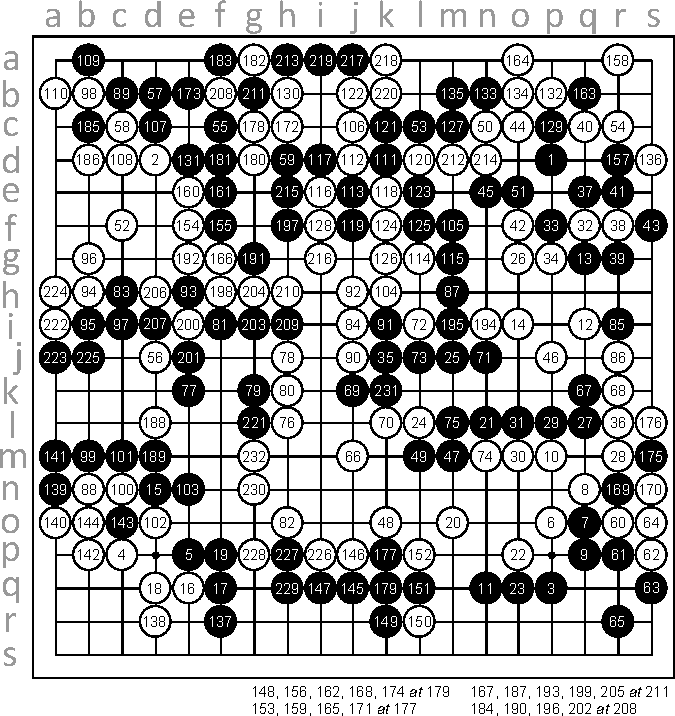
\includegraphics[scale=0.8]{figures/gofirstmove/figKifu.pdf}
\caption{A complete game record, with SGF coordinates, for a 1978 game between Japanese professionals Takemiya Masaki and Kudo Norio.  White (Kudo) won by resignation after 232 moves.  This match has significance in the opening move innovation race, as described in Section \ref{sec:Arms}.}
\label{fig:Kifu}
\end{center}
\end{figure}
 
Go games are quite easy to record, requiring only a single picture of the board at the end of the game, annotated with the sequence of moves played and notes for any stones that were removed (e.g. Figure \ref{fig:Kifu}).  Game records from top players and important tournaments have appeared in Japanese newspapers since the turn of the 20th century, often with professional commentary, and are now regularly published online as well.  In addition, many books of problems and strategies are avaliable in East Asia, usually written by active or retired professional players.  Topics in the Go literature range from analysis of specific moves or tactics to broader strategic ideas about play.  One common feature of studying the game is learning proverbs, which impart general lessons about good and bad play in a simple heuristic fashion \footnote{Examples from Segoe Kensaku's \textit{Go Proverbs Illustrated} \citeyearpar{Segoe1960} include ``When your opponent has two weak groups, attack them both at once.'' and ``One point in the center is worth ten in the corner.''}

Digital records of game records have become standardized using the SGF (``Smart Game Format'') markup to document move sequences and metadata in plaintext files.  Though large archives of professional games, stretching back centuries, exist in East Asia, only a fraction have been digitized.  In recent years, tens of thousands of amateur games are played each year on the internet, many of which are freely available in massive online SGF repositories.    

Two British Go historians, John Fairbairn and T Mark Hall, maintain a commercially available SGF database of professional games (``Games of Go on Disk'', or GoGoD) stretching back centuries.  Fairbairn and Hall have conducted extensive commentary and analyses of their database and have made their results freely available online.  One anecdote from their papers is quite telling: for a particular opening pattern\footnote{In SGF notation, \texttt{B[pd]W[dp]B[pp]W[dd]B[pj]W[nc]B[pf]W[jd]}; a less common variant pattern switches Move 2 and Move 4.}, master 20th century player Go Seigen\footnote{Japanese player names throughout this paper are written surname first, followed by given name.} remarked in a 1996 interview that the eighth move by White at SGF board coordinate jd was poor.  Fairbairn and Hall report that 

\begin{quote}
...a database search revealed, in over 120 games, that just about every top pro had played White 8 in this position. Indeed, the very first to do so was... Go Seigen (in 1936). More alarmingly, White had a whopping 56\% winning rate - that is unusually large...[however] when Go made this comment...around 1996, virtually all pros suddenly stopped playing White [at this position]. \citep{Fairbairn2009}
\end{quote}

Such descriptions are tantalizing evidence that professional Go game records contain clear evidence of the social learning dynamics thought to drive much of cultural evolution.  The international professional community is small enough for information to spread quickly from person to person, and most (nearly 90\%) professional players can be connected by one or two links in a match network in the GoGoD database.  Indeed, we assert that the essential features of professional Go - wide-open strategy space, clear performance measures, cumulative innovation, steep learning curve, pervasive norms of action, large community of players, and strong financial and social incentives for success - make it an ideal model system for studying how culture evolves in its broadest sense.  

To that end, we have developed software in the \texttt{R} computing language to aid in the analysis of SGF game archives (the \texttt{kaya} package).  In this analysis, we limit ourselves to 34,251 professional games drawn from the GoGoD archive, spanning the years 1956 to 2009.  Because our focus here is on the behavior of players over their careers, we excluded players with fewer than 50 games on record for Black, leaving 207 unique players.

\subsection{Historical Patterns of Opening Play}

Throughout a game of Go, the players can place their stones at virtually any open grid intersection.  Yet almost all competitive games follow the same basic pattern: initially, Black and White play in the four corners of the board, a few grid lines away from the board's edge (Figure \ref{fig:Heat}).  Play continues along the corners and sides until after the first 50 moves, at which time the players focus on the center of the board, for the main battles of the game.  About 42\% of games in the database end before Move 200, but if they continue, the average focus of play moves towards the outer edge of the board where the last few points of territory are claimed.  

Despite having the maximum number of possibilities, the first few moves of the game are actually the most predictable.  The opening period of the game is often characterized by highly normative, canalized play, where Black and White often follow one of a set of memorized move sequences called \textit{joseki} (or \textit{jungsuk} in Korea), thought to grant neither player a major advantage.  As with Chess openings, strong players maintain an encyclopedic knowledge of explored routes once a particular \textit{joseki} pattern has started.  


\begin{figure}[t]
\begin{center} 
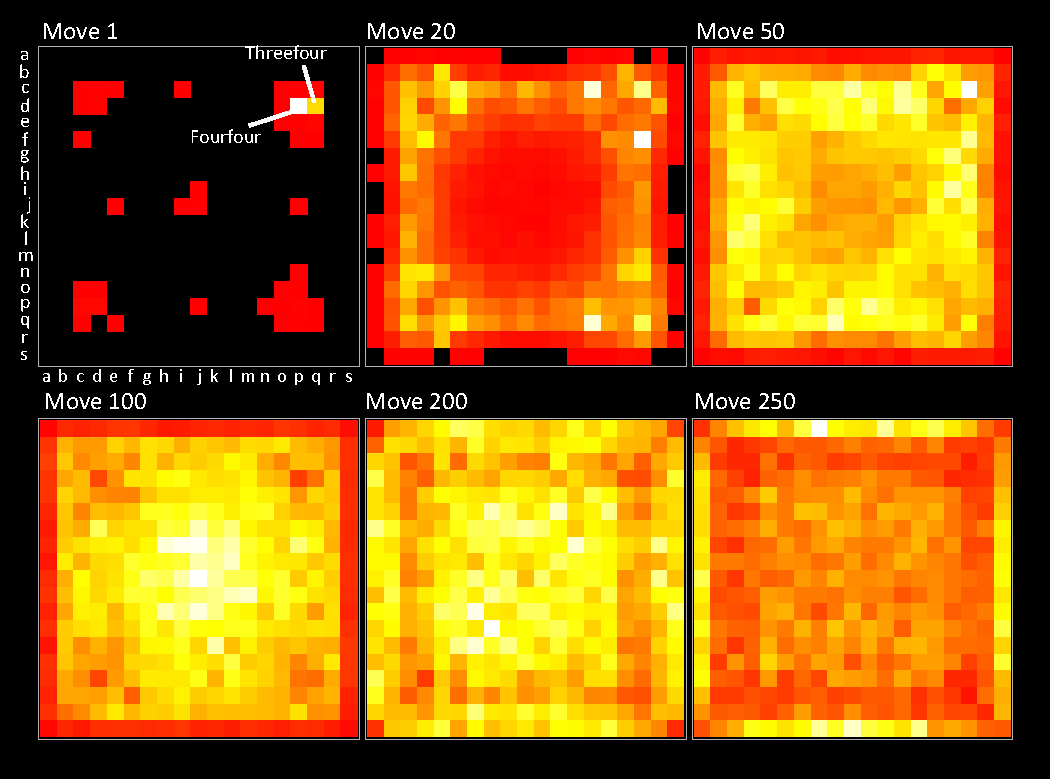
\includegraphics[scale=0.6]{figures/gofirstmove/figHeat.pdf}
\caption{Distribution of database play at six points in the game, showing the most common (white) to least commom (red) board positions.  At Move 1, most locations on the board are unplayed across professional games, and only two are regularly chosen: the Fourfour and the Threefour (whose names are based on the number of grid lines away from the corner).  By Move 20, play has extended to all over the board but remains concentrated in the corner positions.  This continues to the sides of the board, which are the major focus of Move 50.  The midgame, represented by Move 100, concentrates focus on the center of the board, which continues through to Move 200, at which point the entire board is in play and the game approach the maximum entropy value of 361.  Nearing endgame, play moves out towards resolving edge positions.}
\label{fig:Heat}
\end{center}
\end{figure}	
  
We can quantify the importance of these early-game norms in professional play.  A useful way ecologists and physicists measure diversity is using the Shannon index (also called Shannon entropy, or the Shannon-Weiner index), which simultaneously incorporates both the richness and relative evenness of possible options (distinct species, alphanumeric characters, particle positions, etc.; see \citealt{Begon2006}).  In a Go game database, we observe a variety of different locations played for Black's first move.  For $n$ different Move 1 (or M1) variants, each appearing with frequency $p_j$, the Shannon diversity index for M1 is
	\[ 	H' = \exp\bigg( - \sum^{n} p_j \log(p_j) \bigg).
\]
The exponentiation, while not standard, has the advantage of providing a maximum index value of $n$. As a consequence, $H'$ values can be interpreted as the ``effective'' number of options used by players.  In the database used here, the $H'$ value for M1 is 2.86 effective options.  The two dominant M1 variants are the Fourfour and the Threefour (named after their numerical coordinates; see Figure \ref{fig:Heat}, Move 1), with the Threethree a much less common third option.  Calculating the $H'$ for Move 2 (White's first move, responding to Black's M1) gives 6.05 effective alternatives.  If we do this for each game move over all games in the GoGoD database and compare it to the theoretical maximum of 361, it is clear that professional players limit themselves to only a small fraction of possible options within the first 50 moves of the game (Figure \ref{fig:Shannon}).    

\begin{figure}[t]
\begin{center} 
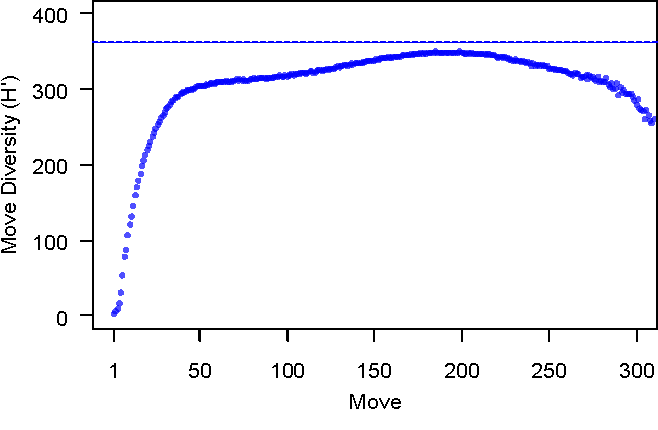
\includegraphics[scale=1.0]{figures/gofirstmove/figShannon.pdf}
\caption{Shannon diversity by game move over the professional database.  For each game move to Move 300, the diversity is calculated via $\exp(-\sum p_j \log(p_j))$, where $p_j$ is the relative frequency of the $j$th variant at that move.  The game eventually approaches a diversity value of 349.23 effective variants at Move 199, indicating that mid-game moves are played at each of 361 intersections on the board with roughly equal frequency across database games.}
\label{fig:Shannon}
\end{center}
\end{figure}

Despite the conservatism of opening play in professional games, novel variations appear regularly and, if widely copied, become new \textit{joseki} in the canon.  Go historian Peter Shotwell writes of the evolution of \textit{joseki}: ``Some are hundreds (or thousands) of years old; others are born, die, and then are reborn again as the style of play changes; still others are yet to be born and patiently wait their turn to be discovered in some flash of ingenuity or desperation.'' \citep{Shotwell2003}

As shown in Figure \ref{fig:M1Freqs}, we can see such dynamics at Move 1 over the latter half of the 20th century.  After a brief enthusiasm for the Threethree in the 1960s, the Fourfour rose to dominance, peaking in 1978 (appearing in 77\% of games played) and again in 1996 (82\% of games played).  As a consequence of these oscillations in the M1 alternatives, we can divide professional play since the 1950s into four major periods (hereafter marked I-IV).  The primary goal of this analysis is to understand why this pattern exists, and what processes are driving its evolution.


\begin{figure}[t]
\begin{center} 
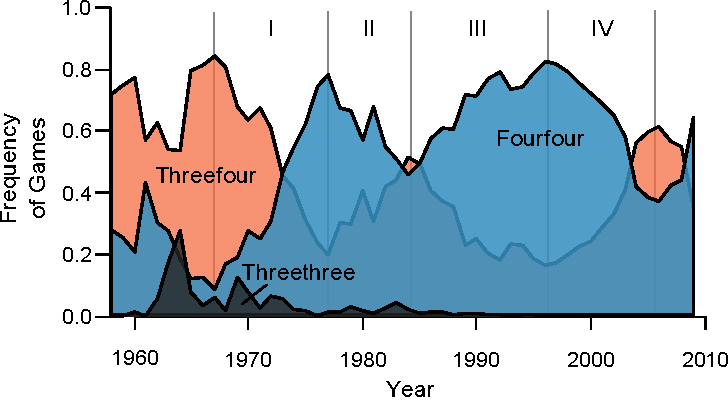
\includegraphics[scale=1.0]{figures/gofirstmove/figM1Freqs.pdf}
\caption{Relative appearance of different variants at Move 1 in the database since 1956.  Because of board symmetry, the M1 Fourfour variant can appear in four different places, and the M1 Threefour variant can appear in eight; the frequencies above take all such congruencies into account.  Based on the cyclic rise and fall of the Fourfour, we can describe four major periods (labeled I-IV) over 20th century professional play.}
\label{fig:M1Freqs}
\end{center}
\end{figure} 
 
 
\section{Cultural Change: Learning versus Demography?}

In general, we consider a cultural trait to \textit{undergo evolution} whenever its distribution within the population changes.  In attempting to explain the oscillatory prevalence of the Move 1 variants over the second half of the 20th century, as described by Figure \ref{fig:M1Freqs}, we can consider a wide variety of underlying evolutionary mechanisms.  Foremost, the enormous amount of study needed to become a professional-level player implies that learning, especially learning from others, is an important source of evolutionary change in Go.
  
Yet, even though standard cultural evolutionary models focus on such social learning, it is important to keep in mind that the distribution of cultural variants in a population can also change due to more ``demographic'' processes.  A change in the age structure, differential migration across the population boundary, or a change in the location of the boundary itself may all bring about cultural change, even though none would be considered ``learning'' or necessarily involve social influence.  If we can establish that the rise of the Fourfour in Period I (1967-1977) is due to, for example, a wave of young Fourfour users joining the professional ranks, then our focus should be the reasons behind this influx, rather than the relatively unimportant learning events taking place within the database.

So, before considering more sophisticated questions about social influence, we have a much more basic and essential task: is the changing prevalence of the Fourfour driven by players altering their behavior (which we'll refer to generically as ``learning''), or is it more due to the demographic replacement of older players as they retire from play with newer players, who enter with a different repertoire of moves?  

The methodology to answer this question is what we call \textit{evolutionary decomposition}, as developed by Coulson and Tuljapurkar \citeyearpar{coulson2008dynamics}, and Beheim and Baldini (in press).  This approach uses individual-level information to exactly partition aggregate change into distinct categories of process.  In Go, there are really only two ways the population can change size: player entry or exit.  Thus, for time periods of arbitrary length, the number of players active in the next period ($N'$) must be related to the number in the current period ($N$) by 
	\[				N' = N + I - E,
\]
where $I$ is the number of players new to the second period, and $E$ the number from the first period absent in the second.  After dividing both sides by $N$, we can express this nondimensionally as 
	\[				G = 1+ i - e.
\]
where $G=N'/N$, $i=I/N$ and $e = E/N$.  If we define player $j$'s ``phenotype'' as $\phi_j$, and assign a ``1'' if they use the Fourfour within their games of a particular time period, and ``0'' if not, we can similarly relate the total number of Fourfour users in successive time periods by
	\[\phi' = \phi + \phi_I + \delta - \phi_E
\]
where $\phi = \sum \phi_j$, $\phi_I$ represents the total number of Fourfour users who have joined the population within the second time period, and $\phi_E$, the total number who have left the population within that period.  The term $\delta$ represents the net balance of those who adopted the Fourfour and those who abandoned it in that time period.  Given these two equations, we can express the change in mean frequency of Fourfour users within the population, $\overline{\phi} = \phi/N$, as
	\[	G \Delta \overline{\phi} = i(\overline{\phi}_I - \overline{\phi}) + c \overline{\delta} - e(\overline{\phi}_E - \overline{\phi}).
\]
Note that $c=1-e$.  Each of the three terms on the right side of the equation describe distinct categories of evolutionary process.  The first term, $i(\overline{\phi}_I - \overline{\phi})$, captures how the mean phenotype among new players alters the mean phenotype of the population, while $e(\overline{\phi}_E - \overline{\phi})$ measures the effect of differential outmigration.  The effect of phenotypic change among those who remain in the population, which here we call ``learning'', is captured by $c \overline{\delta}$. 

Applying this decomposition equation to the game database allows us to see that the Fourfour rose to prominence in Period I almost entirely through learning on the part of professional players, with neglible effects from new players joining the pro community or others leaving it (Figure \ref{fig:PlayerDecomp}).  Here we used two-year periods, but the result holds for one- or five-year periods.  

This result is quite remarkable, considering the major demographic changes taking place in the population.  For 1956, the database used here holds only 105 games, among 18 Black players.  For 2009, 1,354 games are recorded, among 129 unique Black players.  A large part of the explosive growth in the professional Go community can be attributed to changes in nationality; in the 1950s and 1960s, nearly all professionals played in Japan.  In the subsequent decades, professional organizations were established in Korea and China, and by 2009 only about a third of games played are by Japanese players.  Despite these major changes in the size and definition of the population, the decomposition plot indicates that they had very little direct effect on the evolution of M1 variants.  Individual behavioral change is the dominant explanation, and the nature of this change should be the focus of our attention.  


\begin{figure}[t]
\begin{center} 
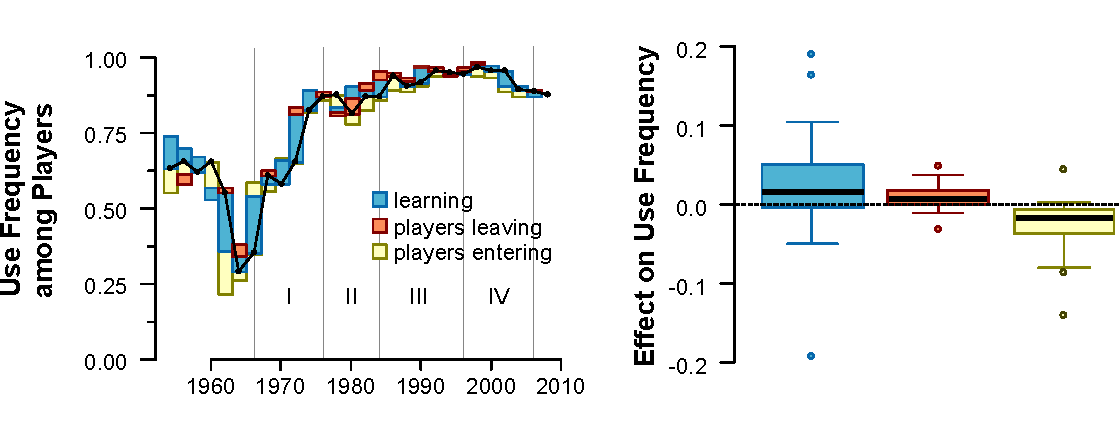
\includegraphics[scale=0.8]{figures/gofirstmove/figPlayerDecomp.pdf}
\caption{Decomposition plot (left) and barplot of decomposition terms (right) for the frequency of use of the Fourfour among players, 1956-2009, using two year periods.  Individual behavioral change (``learning''), rather than population entry and exit, is the dominant explanation of the the rise of the Fourfour during Period I.}
\label{fig:PlayerDecomp}
\end{center}
\end{figure}


% It is naive to think that a single opening move can completely determine victory or defeat, but it is generally understood such moves define the major arc of the game's battles, and are of utmost importance.  

% odd: do the fitted model plots agree with my interpretation of the paraamters??

\section{Are Go Players Social Learners?}

With strong evidence that most of Move 1 evolution in Figure \ref{fig:M1Freqs} can be attributed to professional players altering their behavior (Figure \ref{fig:PlayerDecomp}), we now wish to build a better sense of what motivates such changes.  As strategic actors in a highly competitive environment, Go players are under immense pressure to choose effective moves that help defeat their opponents.  Drawing upon the standard methods in economic and evolutionary theory, we can consider Black's choice at M1 as the result of several plausible models of strategic decision-making \citep{bowles2006microeconomics}.  

(i) \textit{Forward-looking strategic calculation.}  In this model, we imagine rational players who can accurately estimate the future outcomes of particular actions given a set of key input variables, including information about one's general skill compared to that of one's opponent.  Players may choose to try unorthodox or riskier moves against a weaker opponent, who may be less likely to capitalize on their flaws, or when they face a higher handicap.  In such a decision-making model, it is as if the players have complete knowledge of the consequences of using the Fourfour or Threefour variant at Move 1, and simply require the right cues to determine which is best.

(ii) \textit{Recent personal experience.} An obvious problem with forward-looking rationality is that most players cannot realistically determine the value of a move without knowledge of its past use.  Recent experience may show the arrival of a counterstrategy renders a particular move ineffective, and we should expect that players update their valuation of Move 1 variants based on their own past experiences.  

Since records of professional games are widely available (with many of the games taking place in the same locations in Japan and Korea), and the effectiveness of particular choices are difficult to assess from personal experience, we should also expect players to draw upon the information contained in the experiences of others, which we will call ``population knowledge''.  The theoretical literature has concentrated on two simple ways this can be done \citep{boyd1985culture, mcelreath2008beyond}.

(iii) \textit{Success-biased social learning.}  A move that is associated with greater success among other users, regardless of its popularity, may be favored by a focal player.  Similarly, decision-makers may emulate the moves of successful players.  In each case, this strategy rests on a casual association between trait use and the success cue, and so the recent population performance of a particular move should help predict its future use.

(iv) \textit{Frequency-dependent social learning.}  Assuming that players tend to abandon ineffective moves, the prevalence of a move within the Go community itself may be a useful signal of its future performance.  In such situations, we may expect players to simply adopt moves in proportion to their current popularity in the population (``unbiased'' frequency-dependence) or disproportionately favor dominant moves (so-called ``conformity'' bias).  

In both of these cases, players are attending to the experiences of other users, and we should be able to improve our predictions of their behavior by utilizing this information.  Using statistical modeling techniques, we can evaluate how consistent real players are with the idealized models just described, by focusing on three research questions:

\begin{enumerate}
\item Do players employ a particular move coincident with certain features of the match?  If so, what?  The relative ages or recent win records of the players?  The opponent's familiarity with the variant under consideration?
\item Do players tend to respond to their own personal histories with the move?  Are they more likely to play it given past success, or if they have seen it deployed effectively against them in past matches? Could the importance of personal experience with the variant change depending on the focal player's age or recent overall performance?
\item Do players attend to the recent experience of others in the pro community using the move?  Does this interact with the rank or age of the focal player?
\end{enumerate}


\subsection{Methods}

We model the decision to use the Fourfour variant at M1 via a binomial model with a logistic link function of the probability of use, fitted by maximum likelihood in the R programming language.\footnote{In this analysis, we made much use of Ben Bolker's \texttt{bbmle} and Richard McElreath's \texttt{rethinking} packages.}  For each game $j$, we model whether Move 1 was a Fourfour ($y_j=1$) or not ($y_j=0$) via 
\newpage
	\[ y_j \sim \mathrm{Binomial}(1, p_j),
\]
	\[ \mathrm{logit}(p_j) = a + \textbf{xb},
\]
where \textbf{x} is a vector of predictors constructed from other variables in the game database, and \textbf{b}, the vector of corresponding coefficients.

Three major model families were constructed and tested, each embodying one of the above research questions.  The first, ``Match Information'' uses predictors specific to the match; the player's age, win-loss record overall and against this particular opponent, the handicap given to White.  Players who behave according to this model would be forward-looking strategists who can fully anticipate a move's performance and ignore even their own recent experiences, a kind of ``null model'' for learning.  Given that professional players will prepare for a high-profile match by investing a great deal of time reviewing their opponent's games, and that players may be less likely to use a move they know their opponent has commanding mastery of, we also consider the opponent's experience using the Fourfour at Move 1 as a predictor.  

The second model family, ``Personal Knowledge'', includes both a player's recent use of the Fourfour for Move 1, and how often they won games with it, relative to how often they won games without it.  This model corresponds to the hypothesis that players update their views of the move, based on how familiar it is to them and how many games they have won using it.  Finally, ``Population Knowledge'' models use various predictors constructed from the recent population use of the Fourfour, and the population win rate of the Fourfour relative to its alternatives.  These are true social learning models. 

Predictor variables for each game used a retrospective two-year window from the date the game took place, taking the simple average of values for salient games within that period.  Each predictor representing a use frequency was centered on 0.5, a natural point of interpretation for whether a behavior is in the majority.  Predictors for win rate, in contrast, were centered on the average win rate of alternative variants at that game move.  Games in which a predictor was undefined (e.g. a recent win rate for a player's first game) were set to 0 after centering, to drop them out of the model-fitting process.   

Models were fitted and compared in a two-round fashion.  First, within each model family, a variety of models with different combinations of predictor variables were compared using AIC$_c$ and BIC, with top-performing models advancing to the second round.  In the second round, combinations from different model families were constructed and compared.  The top-performing model for each of the three basic model families, as well as the top-performing combination models, are presented in Table \ref{tab:Coeftab}.  


\begin{sidewaystable}[htbp]
  \centering
  \begin{footnotesize}
    \begin{tabular}{lllllll}
	\hline
    \hline
	     & Match & Personal    &  Population   & Match +  & Personal +  & All  \\
          & Information    & Knowledge    &  Knowledge   & Personal   & Population  & Three \\
    \hline
   	Intercept & 0.25 (0.01) & 0.09 (0.02) & 0.08 (0.02) & 0.07 (0.02) & 0.08 (0.02) & 0.02 (0.02) \\
    Personal Win Rate & -0.24 (0.07) &       &       & -0.20 (0.09) &       &  \\
    $\times$ Age & 0.16 (0.05) &       &       & 0.09 (0.07) &       &  \\
    Opponent Use Rate & 1.23 (0.04) &       &       & 0.21 (0.05) &       &  \\
    Handicap (\textit{Komi}) & -0.08 (0.01) &       &       & -0.02 (0.01) &       &  \\
    Per. Use Rate &       & 2.70 (0.11) &       & 2.67 (0.11) & 2.31 (0.11) & 2.30 (0.11) \\
	$\times$ Age  &       &       &       & -0.14 (0.10) &       &  \\
    $\times$ Per. Use Win Rate &       & 0.11 (0.17) &       &       &       &  \\
    (Per. Use Rate)$^2$ &       & 0.28 (0.17) &       & 0.39 (0.17) & 0.29 (0.17) & 0.31 (0.17) \\
    (Per. Use Rate)$^3$ &       & 7.33 (0.61) &       & 6.35 (0.62) & 7.62 (0.62) & 6.79 (0.62) \\
    $\times$ Age &       &       &       & 2.61 (0.53) &       &  2.23 (0.23) \\
    Per. Use Win Rate &       & 0.47 (0.07) &       & 0.39 (0.05) & 0.47 (0.07) & 0.39 (0.05) \\
    (Per. Use Win Rate)$^3$ &       & -0.22 (0.16) &       &       & -0.24 (0.16) &  \\
    Population Use Rate &       &       & 3.06 (0.17) &       & 0.27 (0.19) & 0.32 (0.19) \\
    $\times$ Pop. Use Win Rate &       &       & 9.02 (1.68) &       & 11.04 (1.88) & 9.34 (1.74) \\
    $\times$ Age &       &       &       &       &       & -0.27 (0.07) \\
    $\times$ Per. Use Win Rate &       &       &       &       &       & -1.19 (0.46) \\
    (Pop. Use Rate)$^2$ &       &       & -0.81 (0.43) &       & -1.20 (0.49) &  \\
    (Pop. Use Rate)$^3$ &       &       & 11.95 (2.14) &       & 9.34 (2.36) & 10.48 (2.28) \\
    Pop. Use Win Rate &       &       & 2.30 (0.33) &       & 2.09 (0.37) & 1.82 (0.36) \\
    (Pop. Use Win Rate)$^2$ &       &       & -8.41 (4.28) &       & -10.04 (4.89) &  \\
    \hline
    Validation Error & 38.94 (0.82)  & 26.81 (0.65)  & 34.00 (0.68) & 26.72 (0.66) & 26.63 (0.65) & 26.70 (0.74) \\
    Neg. log Likelihoods & 22586.25 & 18111.59 & 21121.34 & 18054.59 & 17982.01 & 17936.31 \\
    AIC$_c$ weight & $<$0.001  & $<$0.001     & $<$0.001     & $<$0.001     & $<$0.001     &  .99 \\
    \hline
    \end{tabular}%
	\caption{Estimates and standard errors for the top model in each of the three basic model families, plus three combination families.  Both AIC$_c$ and BIC nominate the top model in the ``All Three'' family unequivocally, though the only surviving predictor variables in this model from ``Match Information'' are age interactions.  Model comparison was also done through 10-fold cross-validation, resulting in logistic error rates for each model lower than the baseline error of 41.1\%.}
	\label{tab:Coeftab}%
    \end{footnotesize}
\end{sidewaystable}%


\subsection{Results}

Unsurprisingly, a player's recent use of the Fourfour at M1 strongly predicts their current use: using the ``divide by four'' rule to interpret logistic regression coefficients, a 10 percent difference in past use corresponds to, at most, a 6 percentage point difference in the probability Black will deploy the Fourfour in the current game.  Past personal success with the Fourfour is also predictive, but not as much; an otherwise average player who wins 60\% of their Fourfour games will be about one percentage point more likely to use the Fourfour than a similar player who wins 50\% of recent Fourfour games.  

By itself, the population's recent use of the Fourfour is not as predictive of Black's behavior on M1.  When the Fourfour appears in 60\% of all recent games, the expected probability of use by an average player is only 0.52, compared to 0.50 when the Fourfour appears in half of recent games (Figure \ref{fig:mABCplots}).  However, it is a mistake to think population use is unimportant; it has a large interaction with the Fourfour's relative win rate in the population.  If the Fourfour is at 60\% use and its performance is 10 percentage points higher than that of its rival, the Threefour, the expected probability of use is now 0.58, slightly larger than an equivalent situation for personal use and performance.  

This interaction between popularity and performance in recent games is in fact the largest effect in the top model, strong evidence towards the view Go players are social learners.  But the interaction implies this social learning is \textit{strategic}.  Players are insensitive to a move's popularity when it performs about as well as its rivals, but appear to be quite responsive to the popularity of a high-performing move (Figure \ref{fig:mABCplots}). 

Interestingly, age diminishes the effect of population knowledge but strengthens that of personal knowledge.  In the above scenario (60\% pop. use and $+$10\% pop. win rate) and under the ``All Three'' model, an otherwise average professional in their late teens will use the Fourfour with probability 0.59, while a similar player in his early sixties will only use it with probability 0.56.  In contrast, age strengths the predictive importance of one's personal past use slightly, about half a percentage point for a difference in age of ten years.  

Taken together, this could reflect the behavioral consequences of aging; older players are less willing to change their behavior and less sensitive to trends in the population.  However, older players also tend to be self-selected by performance and rank, so this could alternatively reflect a difference in underlying skill that is present throughout their careers.

Several predictors that were included in each of the early rounds never made it to reported models, including the number of matches played against the current opponent, how successful that opponent has been with the Fourfour recently, the proportion of those matches won, the number of matches in which the Fourfour was used against the focal player (playing as White).  Notably, the population size (i.e. number of active players) itself was predictively irrelevant, both as a main effect and in regulating the importance of population use rate and population use win rate via interactions.

Also noteworthy is that almost all of the ``match-specific'' predictors were excluded in the best-performing model.  Opponent's use of the Fourfour, a strong positive predictor in the ``Match Only'' family, drops out completely once personal knowledge and population knowledge are included.

\begin{figure}[tp]
\begin{center} 
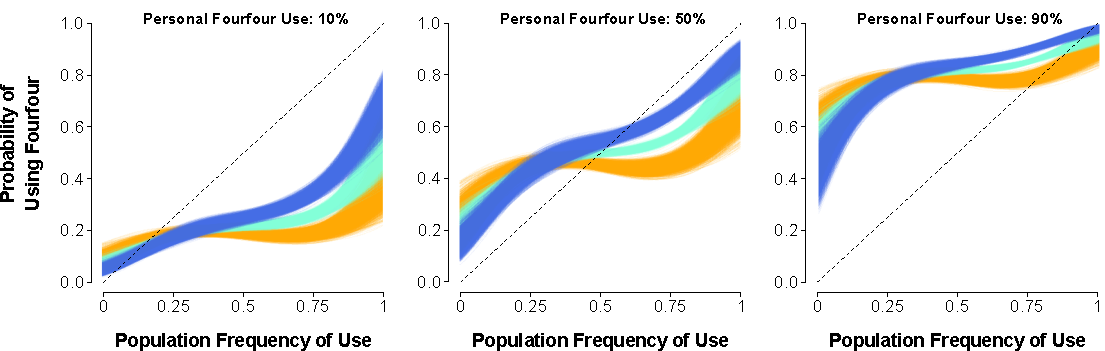
\includegraphics[scale=0.8]{figures/gofirstmove/figmABCplots.pdf}
\caption{Predicted probability of using the Fourfour from the top-performing model, ``All Three'', with uncertainty described by sampling from the joint posterior 5,000 times.  In each panel, the model predicts a response to differences in population use of the Fourfour at three levels of population performance: 10 percentage points better than alternatives (blue), 10 percentage points below alternatives (orange) and performance equivalence (aquamarine).  Players are predicted to be more insensitive to population frequency values when the Fourfour performs about the same as its alternatives at M1.}
\label{fig:mABCplots}
\end{center}
\end{figure}

As demonstrated in Figure \ref{fig:FourfourPredicted}, the ``All Three'' model provides an excellent reconstruction of the observed periodic trajectory of the Fourfour.  Ignoring population knowledge misses the major swings at the zenith and nadir of each cycle, while ignoring personal knowledge produces wide prediction intervals.  Additionally, our top model from the``All Three'' family has an error rate of 26.5\% on the observed data, down from the baseline error rate of 43\%.  Similar values were recovered through ten-fold cross-validation, in which the fitted model makes predictions on new data it has never seen (Table \ref{tab:Coeftab}).
			
% It spread in large part because other players were winning games with it.  This is a broad sketch of a deep story, as the opening move is not in isolation, but associated with.  The win rate with the move seems to indicate that innovative openings using the move allowed it to take off and succeed.  

% So what was difference about 1967 and 1977?  Few people used the move, but those that did saw a remarkable increase in performance, which drove its popularity.  The majority of this effect was social - people saw others doing well using the move.  At its peak in 1977, the interaction between use and wining resulted in a very large effect indeed.  It really was winning more.  Once this trend reversed in the early 80s, the Fourfour waned.


\begin{figure}[t]
\begin{center} 
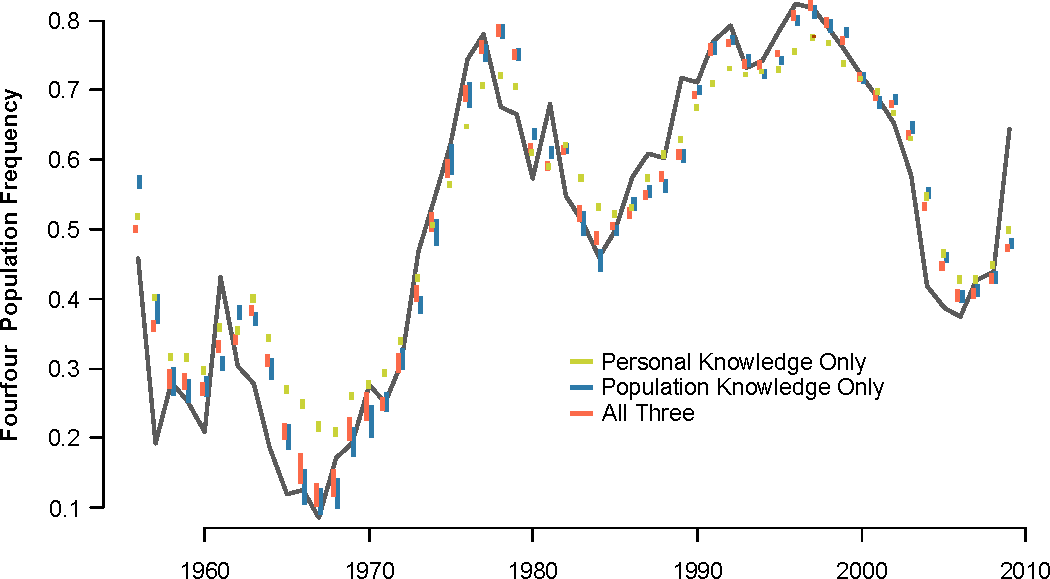
\includegraphics[scale=0.7]{figures/gofirstmove/figFourfourPredicted.pdf}
\caption{The observed and predicted prevalence of the Fourfour variant over time, with each bar spanning the 95\% prediction interval around the maximum likelihood estimate.  Green is the trajectory predicted by the ``Personal Knowledge'' model.  It has a lower logistic error rate (27\%) but does not track population trends closely.  The ``Population Knowledge'' population model (blue) tracks the observed trends more accurately but has wide prediction intervals.  The full model, ``All Three'' (red) is more accurate than personal history alone, since it includes the recent behavior of others, but it is more precise than population history alone.}
\label{fig:FourfourPredicted}	
\end{center}
\end{figure}



\section{Arms Races and Innovation Cycles} \label{sec:Arms}

% cite Boyd and Richerson 1992 on "how microevolutionary processes give rise to history" - the key is the relationship between historical events and process summaries requires you talk about both
 
To summarize, the above has established that (1) most of the change in the prevalence of the Fourfour variant at Move 1 over time is due to learning, rather than demographic changes, and (2) individuals appear to judge a particular variant using social knowledge, namely its overall popularity and relative success.

Despite the fact that the first move of the game hundreds of moves long does not guarantee victory or defeat, how well a particular M1 variant does relative to alternatives within the population is a robust predictor of use.  As indicated by the ``All Three'' model, the Fourfour enjoyed an anomalously large win rate in Period I, during which it proliferated rapidly in the professional community (Figure \ref{fig:M1FreqsWins}).  Conversely, when it declines in Period II, its win rate is consistently below that of its rival variant, the Threefour.

This connection to performance aids our ability to explain the historical record, but we cannot yet say \textit{why} this performance difference exists in the first place, and why the Fourfour did relatively well during Period I and III, but poorly in Period II and IV.  Without the knowledge and skills of a professional player, this may be impossible to fully answer.  However, it is possible to trace the sucess of the Fourfour of 20th century play to particular individuals and events.  From this evidence, it appears that the waxing and waining success of the Fourfour appears to stem from an ongoing crucible of innovation and counterinnovation.

\subsection{Period I: Initial Rise, 1967-1977}

 \begin{figure}[t]
\begin{center} 
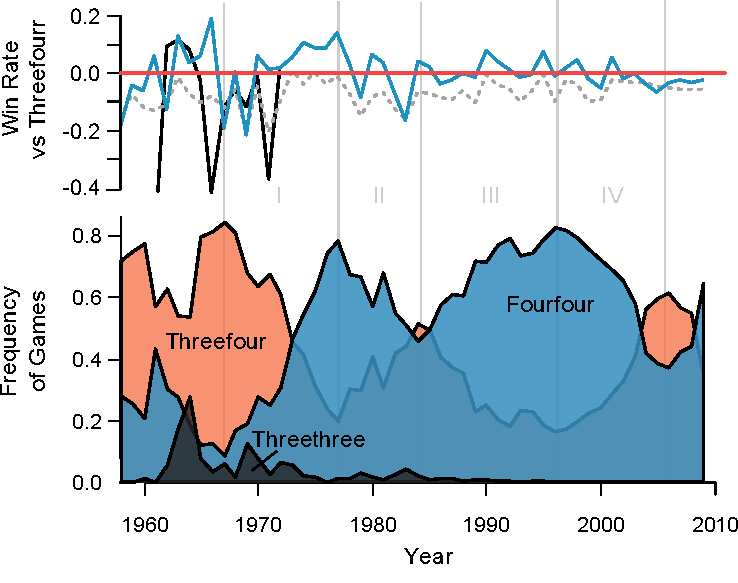
\includegraphics[scale=1.0]{figures/gofirstmove/figM1FreqsWins.pdf}
\caption{The ebb and flow of the three major first move variants, with proportion of games won.  The Fourfour's rise and fall closely tracks with its relative performance (blue line) since 1967.  Similarly, the Threethree's brief efflorescence and extinction closely match its relative win rate (black line).  Because of its initial dominance, all win rates are expressed relative to the Threefour's (red line), and the dotted gray line indicates the location of the 50\% (break-even) point.}
\label{fig:M1FreqsWins}
\end{center}
\end{figure}
 
\begin{figure}[t]
\begin{center} 
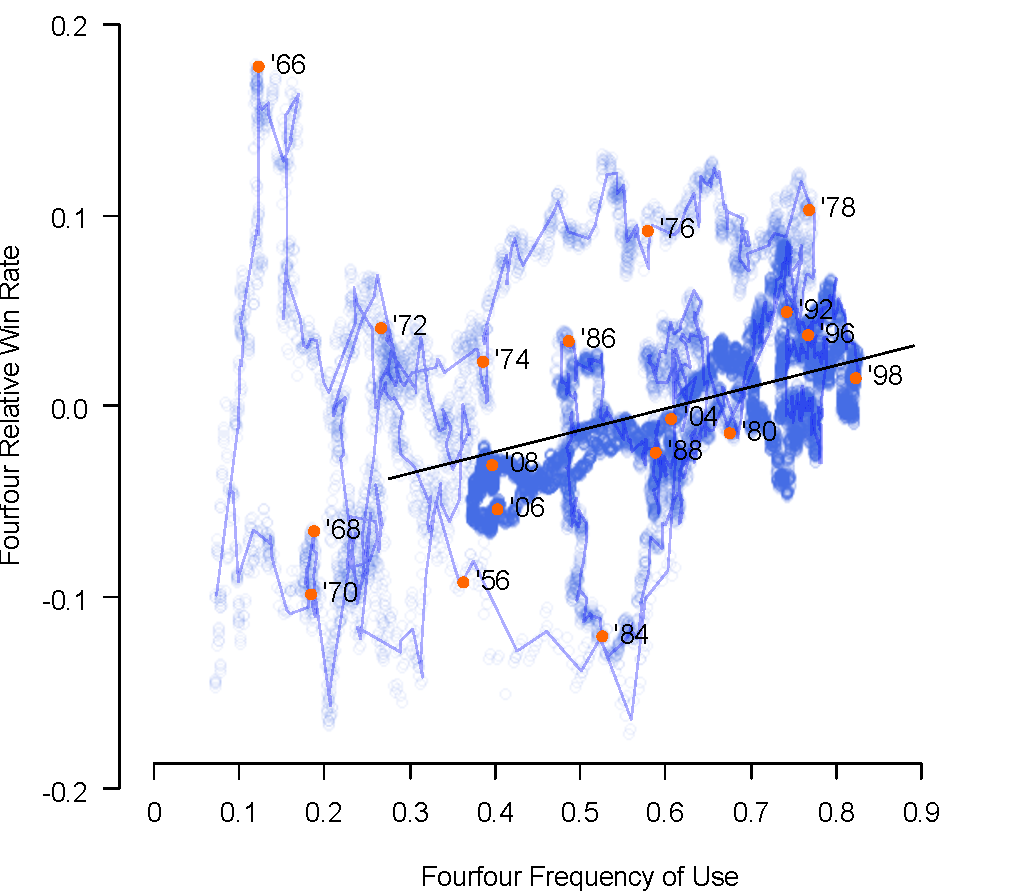
\includegraphics[scale=0.75]{figures/gofirstmove/figSuccessCycle.pdf}
\caption{Recent use of the Fourfour plotted against its recent win rate (r=0.45, with fitted OLS line).  Since its rapid diffusion in the 1970s, the Fourfour's prevalence at M1 has settled into a regular cycle between popularity/success (1978, 1996) and unpopularity/underperformance (1984, 2006).  If this pattern holds, the next peak in popularity should be sometime around 2016.}
\label{fig:SuccessCycle}
\end{center}
\end{figure}

\begin{figure}[t]
\begin{center} 
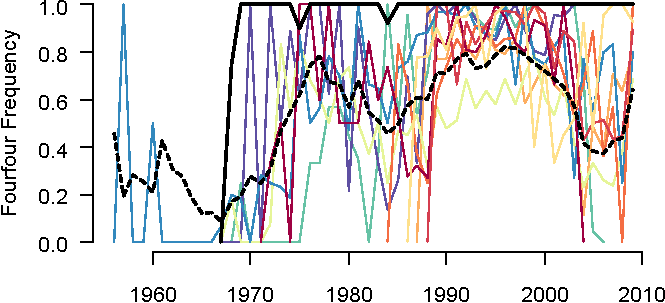
\includegraphics[scale=1.0]{figures/gofirstmove/figPersonalFourfour.pdf}
\caption{Percent of games using Fourfour by population (dashed black line) and by player (colored lines) for the ten most prolific users of the Fourfour.  Takemiya Masaki, who almost always uses the Fourfour, appears as a solid black line.}
\label{fig:PersonalFourfour}
\end{center}
\end{figure}
 
Among Go professionals, one player seems most responsible for the rise of the Fourfour in the 1960s and 1970s: Takemiya Masaki.  Beginning his professional career at the age of 14, Takemiya arrived at the Fourfour's nadir in 1965, and in the database he began using it in 1968.  Takemiya's loose, center-oriented playing style, widely known as ``Cosmic Go'', involves the Fourfour at Move 1 almost exclusively; among his 520 games as Black in the database, only 6 do not start with the Fourfour at M1\footnote{Of these, four are Threefour, one is Threethree, and one is Fourfive.}.  Takemiya's use of the Fourfour coincides with the beginning of Period I and its proliferation within the broader Go community (Figure \ref{fig:PersonalFourfour}).  During this time, his personal performance as Black (61.8\%) also exceeded the average win rate for Black (59\%).  

His influence in starting this trend is apparently a known fact among professionals themselves.  In a 1994 interview with the British Go Journal, Korean master player Seo Pong-su noted that, ``Before him [Takemiya], Korean amateurs and professionals used to avoid the 4-4 point; now this is the most popular opening.'' and attributed Takemiya's innovative play to his greater willingness to research vague, risky moves \citep{Finch1994}.	    

It is interesting to note that the Fourfour was used at M1 before the 1960s, and Takemiya is obviously not its inventor.  However, its success and rapid diffusion is consistent with the hypothesis that Takemiya and his successors hit upon a \textit{new way to use} the Fourfour within the subsequent moves of the game, and this development has had a major effect on strategic landscape of professional Go.

\subsection{Period II: Counterinnovation and Decline, 1977-1984}

 \begin{figure}[t]
\begin{center} 
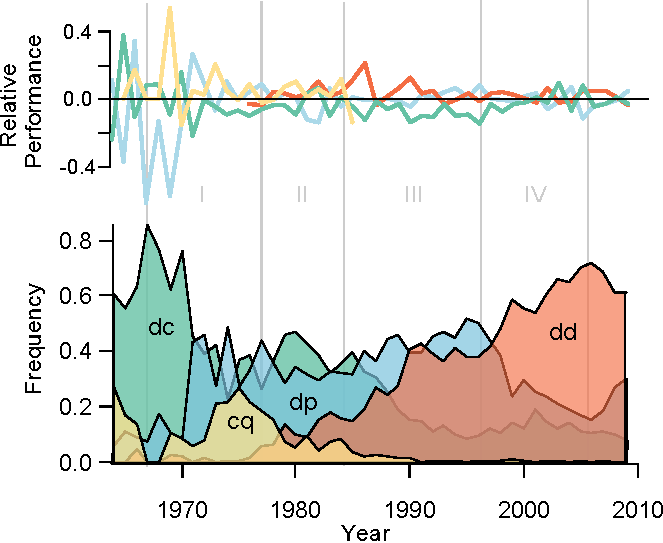
\includegraphics[scale=1.0]{figures/gofirstmove/figM2FreqsWins.pdf}
\caption{Frequency and performance for four major M2 responses to the Fourfour.  Performance for each is calculated as the win rate subtracting the average win rate of alternatives.  As at M1, a variants's frequency closely tracks its relative performance.}
\label{fig:M2FreqsWins}
\end{center}
\end{figure}

Subsequent to Takemiya's arrival, the success of the Fourfour appears to have prompted an innovation race in White's Move 2 response.  Before 1970, White's response to the  Fourfour was almost always a Threefour on an adjacent corner.  If we imagine the M1 Fourfour is played in the upper right quadrant (SGF coordinate pd), nearly 80\% of the time the M2 response in the late 1960s was coordinate dc (Figure \ref{fig:M2FreqsWins}).  By 1977, at the Fourfour's first peak, the M2 dc variant appeared only about 30\% of the time.  During that time, M2 variants dp, cq and dd all became established moves in rapid sequence.  As measured by the proportion of games White won, cq and then dd both consistently outperformed dp during the early 1980s, blunting the Fourfour's effectiveness and anticipating its decline in use.

As with the Fourfour variant at M1, the dd response appeared suddenly, and its early successes can be traced to a single individual, Kudo Norio.  Kudo began using the move in 1977 and won 3 of the 4 games he tried it in (Table \ref{tab:M2dd}).  The next year, he won 4 of 6 attempts, including one against Takemiya (reproduced as Figure \ref{fig:Kifu}).  By 1981, over a dozen professionals were using this M2 variant, and over the next 30 years dd would steadily rise in the professional community to become the dominant response to the M1 Fourfour, followed by dp (Figure \ref{fig:M2FreqsWins}).  It is interesting to note that both of these responses are, by board position, also Fourfours.  

\begin{sidewaystable}[htbp]
  \centering
  \begin{footnotesize}
    \begin{tabular}{rlr|rlr|rlr}
    \hline
	\hline
    1975  & Hasmimoto Utaro & 1 of 1 & 1979  & Cho Chikun & 1 of 2 & 1981  & Cho Chikun & 0 of 1 \\
    1974  & Kato Masao & 0 of 1 &       & Ishida Yoshio & 1 of 6 &       & Fujisawa Hideyuki & 2 of 3 \\
    1976  & Hasmimoto Utaro & 1 of 1 &       & Kobayashi Koichi & 0 of 1 &       & Ishida Yoshio & 1 of 2 \\
          & Takagi Shoichi & 0 of 1 &       & Kudo Norio & 2 of 3 &       & Ishigure Ikuro & 0 of 1 \\
          & Takemiya Masaki  & 0 of 1 &       & Sakata Eio & 5 of 9 &       & Kataoka Satoshi & 1 of 1 \\
    1977  & Cho Chikun & 0 of 3 &       & Takemiya Masaki  & 1 of 2 &       & Ni Linqiang & 0 of 1 \\
          & Hashimoto Utaro & 0 of 1 &       & Ushinohama Satsuo & 2 of 2 &       & Nie Weiping  & 1 of 1 \\
          & Iwata Tatsuaki & 0 of 1 & 1980  & Fujisawa Hideyuki & 2 of 2 &       & Sakata Eio & 2 of 4 \\
          & \textbf{Kudo Norio} & \textbf{3 of 4} &       & Hashimoto Utaro & 0 of 1 &       & Shinkai Hiroko & 0 of 1 \\
          & Takemiya Masaki  & 0 of 3 &       & Ishida Yoshio & 0 of 2 &       & Sugiuchi Masao & 1 of 1 \\
    1978  & Fujisawa Hideyuki & 0 of 1 &       & Kudo Norio & 1 of 1 &       & Takagi Shoichi & 0 of 1 \\
          & Hisai Keishi & 1 of 2 &       & Otake Hideo & 0 of 1 &       & Takemiya Masaki  & 0 of 1 \\
          & \textbf{Kudo Norio} & \textbf{4 of 6} &       & Sakata Eio & 2 of 8 &       & Yamashiro Hiroshi & 1 of 2 \\
          & Magari Reiki & 0 of 1 &       & Takagi Shoichi & 0 of 1 &       &       &  \\
          & Sakata Eio & 0 of 1 &       & Takemiya Masaki  & 1 of 1 &       &       &  \\
          & Ushinohama Satsuo & 0 of 1 &       &       &       &       &       &  \\
    \hline
    \end{tabular}%
	\caption{List of players using the M2 dd move in response to the M1 Fourfour, 1975-1981, with the number of games won out of the number attempted.  Kudo Norio's remarkable success in 1977 and 1978 anticipates the dd variant's proliferation (Figure \ref{fig:M2FreqsWins}).  One of Kudo's winning 1978 games, against the modern pioneer of the Fourfour, is reprinted as Figure \ref{fig:Kifu}.}
	\label{tab:M2dd}%
	\end{footnotesize}
\end{sidewaystable}%



\section{Discussion}

Though only a preliminary treatment of a very rich dataset, the above results demonstrate how a socially-transmitted cultural pattern of behavior - the move variants at M1 and M2 in the game of Go - undergo evolutionary change.  From the above evidence, it seems that the average professional player uses both personal knowledge and social knowledge to decide which move to use in a particular game.  Using evolutionary decomposition, we can show that, despite major growth in the professional community and addition of players from China and Korea, the population dynamics of opening moves is driven by learning on the part of active players, rather than demographic effects from influx of younger players or outflux of older players.  A player's recent use of a move at M1 effectively predicts their future behavior, indicating players update their play based on past experiences.  This association increases with age; older players are better predicted by their play in the last two years than younger players.  Personal win rate using the variant also aids in prediction, but this effect is not as strong as a player's past use. 

We also have evidence that players use population knowledge; a professional's behavior at M1 is strongly predicted by the recent population performance of particular variants.  The population frequency of an M1 variant is also predictive, but only when that variant is, on the average, winning more (or fewer) games than its rivals.  The conditional importance of the Fourfour's popularity seems to indicate that players use the frequency information strategically, since the theoretical advantages of frequency-dependent learning strategies come from an association between popularity and performance.  

Given these results, it should be no surprise that the Fourfour's prevalence is strongly associated with its recent performance since the 1960s.  By looking at particular games, we can also see how the breakaway success of the Fourfour variant at M1 was followed by a period of innovation and diversity in more effective M2 responses.  Taken together, this evidence all seems to indicate an ongoing evolutionary arms race taking place within the opening moves of professional Go.  

Although we can do much to reconstruct and explore the historical record, several important questions remain outstanding.  First, we do not know the nature of the observed success bias.  We can see that relative performance of the Fourfour versus the Threefour consistently improves our predictions of which one a particular player will use.  This seems to indicate players focus on how well a move does, but it is equally possible, however, that successful \textit{players} rather than successful variants are what are emulated.  

This is not captured by crude measures like population use frequency, and is indicative of a larger problem: establishing exactly who players are learning from.  The statistical models above treat the general population as an equally-connected, homogenous pool.  Real social influence in this situation undoubtedly involves a variety of complex social relationships between unique personalities.  The nature of these influences may be better captured by network-based approaches that allow for heterogeneous interconnections between players.  It may be possible to use information about players' nationalities or recent matches to develop measures of social proximity, allowing the detection of theoretical effects like conformist learning or prestige.

Another problem is the nature of innovation in Fourfour play.  Even if Takemiya's ``Cosmic'' opening style was the catalyst for the Fourfour's rise in Period I, as the evidence above seems to indicate, we do not know if other adopters were using it in the same way.  The observed pattern could be, for example, due to Takemiya's early successes in 1968-1970 encouraging other professionals to revisit the Fourfour and develop their own innovative applications, rather than emulate his.  

Finally, even if players really are using a combination of individual and population knowledge, we should consider the possibility that this offers no real strategic advantage.  A well-understood problem with success bias is that it aims to exploit an association between use and performance, but can lead to the proliferation of neutral or even deleterious practices if that association is not causal.  The dynamics described above would exist even if the first move has little impact on the subsequent game, provided only that players \textit{think} it does. 

There are many more possible avenues of exploration in this very rich dataset.  Venturing beyond Move 2, we can study the diffusion of particular \textit{joseki} patterns, the importance of particular high-status individuals (like the Go Seigen interview described above) or, indirectly, the diffusion of particular Go proverbs within profesisonal play.  The scope of study can also be expanded; large archives of professional games go back at least several hundred years, and tens of thousands of amateur games are available online, to say nothing of similar archives available for other games like chess.  

In any case, the statistical and theoretical tools employed above can be used to expand our understanding of cultural dynamics.  The above results hopefully demonstrate the value of taking a quantitative, Darwinian point of view towards cultural change.  As in evolutionary ecology, we can use the results of high-resolution datasets to help understand, indirectly, historical dynamics for which little data remains and variants are harder to define.  Indeed, we feel that the theroetical and empirical evidence is so overwhelming that the key question is not ``whether'' culture evolves, but rather which day-to-day learning and demographic processes brought about the particular patterns of cultural diversity we see in human history.  






% This innovation can also be correlated to the size of the professional community as well.  To put it simply, more individuals means more innovation and faster arms race dynamics.  












\begin{thebibliography}{200}
	\thispagestyle{myheadings}
 %	\addcontentsline{toc}{chapter}{\bibname}
	\bibliographystyle{apalike}     % The style of your bibliography
	
\bibitem[Anderson, 2000]{Anderson2000:Slowboats}
Anderson, A. (2000).
\newblock Slow boats from china: issues in the prehistory of indo-pacific
  seafaring.
\newblock In O'Connor, S. and Veth, P., editors, {\em East of Wallace's Line:
  Studies of Past and Present Maritime Cultures in the Indo-Pacific region}.
  A.A. Balkema, Rotterdam.

\bibitem[Anderson, 2001]{Anderson2001:SharpEnd}
Anderson, A. (2001).
\newblock Towards the sharp end: the form and performance of prehistoric
  polynesian voyaging canoes.
\newblock In Stevenson, C.M., G.~L. and Morin, F., editors, {\em Pacific 2000:
  proceedings of the fifth international conference on Easter Island and the
  Pacific}. Easter Island Foundation, Los Osos.

\bibitem[Anderson et~al., 2000]{Anderson2000:nhst}
Anderson, D.~R., Burnham, K.~P., and Thompson, W.~L. (2000).
\newblock Null hypothesis testing: Problems, prevalence, and an alternative.
\newblock {\em The Journal of Wildlife Management}, 64(4):912--923.

\bibitem[Banack, 1991]{Banack1991ethnobotany}
Banack, S. (1991).
\newblock Plants and polynesian voyaging.
\newblock In Banack, P. A.~C. and Anne, S., editors, {\em Islands, plants, and
  Polynesians : an introduction to Polynesian ethnobotany}. Dioscorides Press,
  Portland, Or.

\bibitem[Barkow et~al., 1992]{Barkow1992adaptedmind}
Barkow, J.~H., Cosmides, L., and Tooby, J. (1992).
\newblock {\em The Adapted Mind: Evolutionary Psychology and the Generation of
  Culture}.
\newblock Oxford University Press.

\bibitem[Baum et~al., 2004]{baum2004cultural}
Baum, W., Richerson, P., Efferson, C., and Paciotti, B. (2004).
\newblock Cultural evolution in laboratory microsocieties including traditions
  of rule giving and rule following.
\newblock {\em Evolution and Human Behavior}, 25(5):305--326.

\bibitem[Begon et~al., 2006]{Begon2006}
Begon, M., Townsend, C.~R., and Harper, J.~L. (2006).
\newblock {\em Ecology}.
\newblock Blackwell Publishing, 4th edition.

\bibitem[Berger and Berry, 1988]{Berger1988}
Berger, J.~O. and Berry, D.~A. (1988).
\newblock Statistical analysis and the illusion of objectivity.
\newblock {\em American Scientist}, 76.

\bibitem[Betzig, 1997]{Betzig1997humannature}
Betzig, L.~L. (1997).
\newblock {\em Human Nature : A Critical Reader}.
\newblock Oxford University Press, New York.

\bibitem[Biggs, 2006]{Biggs2006}
Biggs, B. (2006).
\newblock {\em Kimihia te mea ngaro: Seek that which is lost}.
\newblock The Polynesian Society, Auckland, N.Z.

\bibitem[Bolker, 2008]{Bolker2008}
Bolker, B.~M. (2008).
\newblock {\em Ecological Models and Data in R}.
\newblock Princeton University Press.

\bibitem[Bowles, 2006]{bowles2006microeconomics}
Bowles, S. (2006).
\newblock {\em Microeconomics: Behavior, Institutions, and Evolution}.
\newblock Princeton University Press.

\bibitem[Boyd and Richerson, 1985]{boyd1985culture}
Boyd, R. and Richerson, P. (1985).
\newblock {\em Culture and the Evolutionary Process}.
\newblock University of Chicago Press.

\bibitem[Burnham and Anderson, 2002]{Burnham&Anderson:2002}
Burnham, K. and Anderson, D. (2002).
\newblock {\em Model Selection and Multi-Model Inference: A Practical
  Information-Theoretic Approach}.
\newblock Springer.

\bibitem[Caldwell and Millen, 2008]{caldwell2008studying}
Caldwell, C. and Millen, A. (2008).
\newblock Studying cumulative cultural evolution in the laboratory.
\newblock {\em Philosophical Transactions of the Royal Society B: Biological
  Sciences}, 363(1509):3529.

\bibitem[Campbell, 1965]{campbell1965variation}
Campbell, D. (1965).
\newblock Variation and selective retention in socio-cultural evolution.
\newblock In Barringer, H., Blanksten, G., and Mack, R., editors, {\em Social
  Change in Developing Areas: A Reinterpretation of Evolutionary Theory}, pages
  19--49. Schenkman.

\bibitem[Cashdan and Rogers, 1997]{Cashdan&Rogers1997:review}
Cashdan, E. and Rogers, A. (1997).
\newblock Book review of "human nature: A critical reader".
\newblock {\em Evolution \& Human Behavior}, 18:297--283.

\bibitem[Cavalli-Sforza and Feldman, 1981]{cavalli1981cultural}
Cavalli-Sforza, L. and Feldman, M. (1981).
\newblock {\em Cultural Transmission and Evolution: A Quantitative Approach}.
\newblock Princeton University Press.

\bibitem[Chudek et~al., 2011]{chudek2011prestige}
Chudek, M., Heller, S., Birch, S., and Henrich, J. (2011).
\newblock Prestige-biased cultural learning: Bystander's differential attention
  to potential models influences children's learning.
\newblock {\em Evolution and Human Behavior}.

\bibitem[Cohen, 1994]{Cohen1994}
Cohen, J. (1994).
\newblock The world is round (p $<$ .05).
\newblock {\em American Psychologist}, 49(12):997--1003.

\bibitem[Coulson and Tuljapurkar, 2008]{coulson2008dynamics}
Coulson, T. and Tuljapurkar, S. (2008).
\newblock The dynamics of a quantitative trait in an age-structured population
  living in a variable environment.
\newblock {\em The American Naturalist}, 172(5):599--612.

\bibitem[Dawkins, 2006]{dawkins2006selfish}
Dawkins, R. (2006).
\newblock {\em The Selfish Gene}.
\newblock Oxford University Press.

\bibitem[Diamond, 2002]{Diamond2002domestication}
Diamond, J. (2002).
\newblock Evolution, consequences and future of plant and animal domestication.
\newblock {\em Nature}, 418(6898):700--7.

\bibitem[Doran, 1981]{Doran1981canoes}
Doran, E.~B. (1981).
\newblock {\em Wangka : Austronesian canoe origins}.
\newblock Texas A\&M University Press, College Station, 1st edition.

\bibitem[Durham, 1992]{durham1992coevolution}
Durham, W. (1992).
\newblock {\em Coevolution: Genes, Culture, and Human Diversity}.
\newblock Stanford University Press.

\bibitem[Edgerton, 1971]{Edgerton1971}
Edgerton, R.~B. (1971).
\newblock {\em The individual in cultural adaptation; a study of four East
  African peoples}.
\newblock University of California Press, Berkeley,.

\bibitem[Eerkens et~al., 2006]{EerkensBettingerMcElreath2006}
Eerkens, J.~W., Bettinger, R.~L., and McElreath, R. (2006).
\newblock Cultural transmission, phylogenetics, and the archaeological record.
\newblock In Lipo, C.~P., O'Brien, M.~J., Collard, M., and Shennan, S.~J.,
  editors, {\em Mapping Our Ancestors}. AldineTransactions, London.

\bibitem[Efferson et~al., 2008]{efferson2008conformists}
Efferson, C., Lalive, R., Richerson, P., McElreath, R., and Lubell, M. (2008).
\newblock Conformists and mavericks: The empirics of frequency-dependent
  cultural transmission.
\newblock {\em Evolution and Human Behavior}, 29(1):56--64.

\bibitem[Efferson et~al., 2007a]{efferson2007learning}
Efferson, C., Richerson, P., McElreath, R., Lubell, M., Edsten, E., Waring, T.,
  Paciotti, B., and Baum, W. (2007a).
\newblock Learning, productivity, and noise: An experimental study of cultural
  transmission on the bolivian altiplano.
\newblock {\em Evolution and Human Behavior}, 28(1):11--17.

\bibitem[Efferson et~al., 2007b]{effersontakezawa2007}
Efferson, C., Takezawa, M., and McElreath, R. (2007b).
\newblock New methods in quantitative ethnography: Economic experiments and
  variation in the price of equality.
\newblock {\em Current Anthropology}, 48:912--919.

\bibitem[Eriksson and Coultas, 2009]{eriksson2009people}
Eriksson, K. and Coultas, J. (2009).
\newblock Are people really conformist-biased? an empirical test and a new
  mathematical model.
\newblock {\em Journal of Evolutionary Psychology}, 7(1):5--21.

\bibitem[Fairbairn and Hall, 2009]{Fairbairn2009}
Fairbairn, J. and Hall, T.~M. (2009).
\newblock {\em The Go Companion}.
\newblock Slate and Shell.

\bibitem[Finch, 1994]{Finch1994}
Finch, A. (1994).
\newblock Korean interview.
\newblock {\em British Go Journal}, 96:16--17.

\bibitem[Gaddis, 2002]{Gaddis2002}
Gaddis, J.~L. (2002).
\newblock {\em The Landscape of History: How Historians Map the Past}.
\newblock Oxford University Press.

\bibitem[Gill, 2008]{Gill2008}
Gill, J. (2008).
\newblock {\em Bayesian Methods: A Social and Behavioral Sciences Approach}.
\newblock Chapman \& Hall/CRC, 2nd ed. edition.

\bibitem[Grant and Grant, 2002]{grant2002unpredictable}
Grant, P. and Grant, B. (2002).
\newblock Unpredictable evolution in a 30-year study of darwin's finches.
\newblock {\em Science}, 296(5568):707.

\bibitem[Gravlee et~al., 2009]{gravlee2009methods}
Gravlee, C., Kennedy, D., Godoy, R., and Leonard, W. (2009).
\newblock Methods for collecting panel data: What can cultural anthropology
  learn from other disciplines?
\newblock {\em Journal of Anthropological Research}, 65(3):453--483.

\bibitem[Gray et~al., 2010]{GrayBryantGreenhill2010}
Gray, R., Bryant, D., and Greenhill, S. (2010).
\newblock On the shape and fabric of human history.
\newblock {\em Philosophical Transactions of the Royal Society B: Biological
  Sciences}, 365(1559):3923--3933.

\bibitem[Gray et~al., 2009]{Gray2009:Phylogenies}
Gray, R., Drummond, A., and Greenhill, S. (2009).
\newblock Language phylogenies reveal expansion pulses and pauses in pacific
  settlement.
\newblock {\em Science}, 323.

\bibitem[Guglielmino et~al., 1995]{Guglielmino1995}
Guglielmino, C.~R., Viganotti, C., Hewlett, B., and Cavalli-Sforza, L.~L.
  (1995).
\newblock Cultural variation in africa: Role of mechanisms of transmission and
  adaptation.
\newblock {\em Proceedings of the National Academy of Sciences of the United
  States of America}, 92(16):7585--7589.

\bibitem[Haddon and Hornell, 1936]{HaddonHornell1936}
Haddon, A.~C. and Hornell, J. (1936).
\newblock {\em Canoes of Oceania}.
\newblock Bernice P. Bishop Museum, Honolulu.

\bibitem[Harris, 1968]{Harris1968}
Harris, M. (1968).
\newblock {\em The rise of anthropological theory: a history of theories of
  culture}.
\newblock Routeledge and Kegan Paul Ltd.

\bibitem[Henrich, 2001]{Henrich2001}
Henrich, J. (2001).
\newblock Cultural transmission and the diffusion of innovations: Adoption
  dynamics indicate that biased cultural transmission is the predominate force
  in behavioral change.
\newblock {\em American Anthropologist}, 103(4):992--1013.

\bibitem[Henrich, 2004]{Henrich2004:Tasmania}
Henrich, J. (2004).
\newblock Demography and cultural evolution: How adaptive cultural processes
  can produce maladaptive losses - the tasmanian case.
\newblock {\em American Antiquity}, 69(2).

\bibitem[Henrich and Boyd, 2002]{Henrich2002}
Henrich, J. and Boyd, R. (2002).
\newblock On modeling cognition and culture: Why cultural evolution does not
  require replication of representations.
\newblock {\em Journal of Cognition and Culture}, 2(2):87--112.

\bibitem[Henrich et~al., 2008]{Henrich2008:misunderstandings}
Henrich, J., Boyd, R., and Richerson, P.~J. (2008).
\newblock Five misunderstandings about cultural evolution.
\newblock {\em Human Nature-an Interdisciplinary Biosocial Perspective},
  19(2):119--137.

\bibitem[Henrich and Broesch, 2011]{henrich2011nature}
Henrich, J. and Broesch, J. (2011).
\newblock On the nature of cultural transmission networks: Evidence from fijian
  villages for adaptive learning biases.
\newblock {\em Philosophical Transactions of the Royal Society B: Biological
  Sciences}, 366(1567):1139--1148.

\bibitem[Henrich et~al., 2010]{henrich2010weirdest}
Henrich, J., Heine, S., and Norenzayan, A. (2010).
\newblock The weirdest people in the world?
\newblock {\em Behavioral and Brain Sciences}, 33(2-3):61--83.

\bibitem[Henrich and Henrich, 2010]{henrich2010evolution}
Henrich, J. and Henrich, N. (2010).
\newblock The evolution of cultural adaptations: Fijian food taboos protect
  against dangerous marine toxins.
\newblock {\em Proceedings of the Royal Society B: Biological Sciences},
  277(1701):3715--3724.

\bibitem[Hilborn and Mangel, 1997]{Hilborn1997}
Hilborn, R. and Mangel, M. (1997).
\newblock {\em The ecological detective: confronting models with data}.
\newblock Princeton University Press.

\bibitem[Horridge, 1987]{Horridge1987:IndonesiaCanoes}
Horridge, G.~A. (1987).
\newblock {\em Outrigger canoes of Bali and Madura, Indonesia}.
\newblock Bishop Museum Press, Honolulu.

\bibitem[Hout et~al., 2001]{hout2001demographic}
Hout, M., Greeley, A., and Wilde, M. (2001).
\newblock The demographic imperative in religious change in the united states.
\newblock {\em American Journal of Sociology}, 107(2):468--500.

\bibitem[Irwin, 1992]{Irwin1992}
Irwin, G. (1992).
\newblock {\em The Prehistoric exploration and colonization of the Pacific}.
\newblock Cambridge University Press, Cambridge.

\bibitem[Johnson and Earle, 2000]{JohnsonEarle2000:EvolSocieties}
Johnson, A.~W. and Earle, T.~K. (2000).
\newblock {\em The evolution of human societies : from foraging group to
  agrarian state}.
\newblock Stanford University Press, Stanford, Calif., 2nd edition.

\bibitem[Johnson and Omland, 2004]{Johnson&Omland2004:modelselection}
Johnson, J.~B. and Omland, K.~S. (2004).
\newblock Model selection in ecology and evolution.
\newblock {\em Trends in Ecology \& Evolution}, 19(2):101--108.

\bibitem[Kirch, 1984]{Kirch1984evolution}
Kirch, P.~V. (1984).
\newblock {\em The evolution of the Polynesian chiefdoms}.
\newblock New studies in archaeology. Cambridge University Press, Cambridge.

\bibitem[Kirch, 2000]{Kirch2000:Road}
Kirch, P.~V. (2000).
\newblock {\em On the road of the winds : an archaeological history of the
  Pacific Islands before European contact}.
\newblock University of California Press, Berkeley, Calif.

\bibitem[Kirch, 2007]{Kirch2007}
Kirch, P.~V. (2007).
\newblock Hawaii as a model system for human ecodynamics.
\newblock {\em American Anthropologist}, 109(1):8--26.

\bibitem[Laland and Brown, 2002]{LalandBrown2002sense}
Laland, K.~N. and Brown, G.~R. (2002).
\newblock {\em Sense and nonsense: Evolutionary perspectives on human
  behaviour}.
\newblock Oxford University Press, New York.

\bibitem[Lewis, 1978]{Lewis1978:PacificNavigators}
Lewis, D. (1978).
\newblock {\em The voyaging stars : secrets of the Pacific island navigators}.
\newblock W. W. Norton, New York.

\bibitem[Lumsden and Wilson, 2005]{lumsden2005genes}
Lumsden, C. and Wilson, E. (2005).
\newblock {\em Genes, Mind, and Culture: The Coevolutionary Process}.
\newblock World Scientific Publishing Company.

\bibitem[McElreath, 2004]{mcelreath2004social}
McElreath, R. (2004).
\newblock Social learning and the maintenance of cultural variation: An
  evolutionary model and data from east africa.
\newblock {\em American Anthropologist}, 106(2):308--321.

\bibitem[McElreath et~al., 2008]{mcelreath2008beyond}
McElreath, R., Bell, A., Efferson, C., Lubell, M., Richerson, P., and Waring,
  T. (2008).
\newblock Beyond existence and aiming outside the laboratory: Estimating
  frequency-dependent and payoff-biased social learning strategies.
\newblock {\em Philosophical Transactions of the Royal Society B: Biological
  Sciences}, 363(1509):3515--3528.

\bibitem[McElreath et~al., 2005]{mcelreath2005applying}
McElreath, R., Lubell, M., Richerson, P., Waring, T., Baum, W., Edsten, E.,
  Efferson, C., and Paciotti, B. (2005).
\newblock Applying evolutionary models to the laboratory study of social
  learning.
\newblock {\em Evolution and Human Behavior}, 26(6):483--508.

\bibitem[Mead, 1957]{Mead1957:PolynesianLab}
Mead, M. (1957).
\newblock Introduction to polynesia as laboratory for the development of models
  in the study of cultural evolution.
\newblock {\em Journal of the Polynesian Society}, 66:145.

\bibitem[Mesoudi, 2011]{Mesoudi2011a}
Mesoudi, A. (2011).
\newblock An experimental comparison of human social learning strategies:
  payoff-biased social learning is adaptive but underused.
\newblock {\em Evolution and Human Behavior}, 32(5):334--342.

\bibitem[Mesoudi and O'Brien, 2008]{mesoudi2008cultural}
Mesoudi, A. and O'Brien, M. (2008).
\newblock The cultural transmission of great basin projectile-point technology
  i: An experimental simulation.
\newblock {\em American Antiquity}, pages 3--28.

\bibitem[Mesoudi et~al., 2006]{Mesoudi2006}
Mesoudi, A., Whiten, A., and Laland, K.~N. (2006).
\newblock Towards a unified science of cultural evolution.
\newblock {\em Behavioral and Brain}, 29:329--383.

\bibitem[Michel et~al., 2011]{michel2011quantitative}
Michel, J., Shen, Y., Aiden, A., Veres, A., Gray, M., Pickett, J., Hoiberg, D.,
  Clancy, D., Norvig, P., and Orwant, J. (2011).
\newblock Quantitative analysis of culture using millions of digitized books.
\newblock {\em Science}, 331(6014):176.

\bibitem[Mueller-Dombois and Fosberg, 1998]{Mueller1998:Vegetation}
Mueller-Dombois, D. and Fosberg, F.~R. (1998).
\newblock {\em Vegetation of the tropical Pacific islands}.
\newblock Springer, New York.

\bibitem[Nisbett and Cohen, 1996]{Nisbett1996}
Nisbett, R.~E. and Cohen, D. (1996).
\newblock {\em Culture of honor: the psychology of violence in the South}.
\newblock New directions in social psychology. Westview Press, Boulder, CO.

\bibitem[Ozgul et~al., 2009]{ozgul2009dynamics}
Ozgul, A., Tuljapurkar, S., Benton, T., Pemberton, J., Clutton-Brock, T., and
  Coulson, T. (2009).
\newblock The dynamics of phenotypic change and the shrinking sheep of st.
  kilda.
\newblock {\em Science}, 325(5939):464.

\bibitem[Paciotti and Hadley, 2003]{paciotti2003ultimatum}
Paciotti, B. and Hadley, C. (2003).
\newblock The ultimatum game among sympatric ethnic groups in southwestern
  tanzania: Ethnic variation and institutional scope.
\newblock {\em Current Anthropology}, 44:427--432.

\bibitem[Price, 1970]{price1970selection}
Price, G.~R. (1970).
\newblock Selection and covariance.
\newblock {\em Nature}, 227(5257):520--521.

\bibitem[Rendell et~al., 2011]{rendell2011copying}
Rendell, L., Boyd, R., Enquist, M., Feldman, M., Fogarty, L., and Laland, K.
  (2011).
\newblock How copying affects the amount, evenness and persistence of cultural
  knowledge: insights from the social learning strategies tournament.
\newblock {\em Philosophical Transactions of the Royal Society B: Biological
  Sciences}, 366(1567):1118--1128.

\bibitem[Rice, 2004]{rice2004evolutionary}
Rice, S. (2004).
\newblock {\em Evolutionary Theory: Mathematical and Conceptual Foundations}.
\newblock Sinauer Associates Sunderland.

\bibitem[Richerson and Boyd, 2005]{Richerson2005:NBGA}
Richerson, P. and Boyd, R. (2005).
\newblock {\em Not by Genes Alone: How Culture Transformed Human Evolution}.
\newblock University of Chicago Press.

\bibitem[Rimmel et~al., 2010]{Rimmel2010}
Rimmel, A., Teytaud, O., Lee, C.-S., Yen, S.-J., Wang, M.-H., and Tsai, S.-R.
  (2010).
\newblock Current frontiers in computer go.
\newblock {\em Computational Intelligence and AI in Games, IEEE Transactions
  on}, 2(4):229 --238.

\bibitem[Rogers and Cashdan, 1997]{Rogers&Cashdan1997:phylogeny}
Rogers, A. and Cashdan, E. (1997).
\newblock The phylogenetic approach to comparing human populations.
\newblock {\em Evolution \& Human Behavior}, 18(5):353--358.

\bibitem[Rogers et~al., 2009]{RogersFeldmanEhrlich2009}
Rogers, D., Feldman, M., and Ehr (2009).
\newblock Inferring population histories using cultural data.
\newblock {\em Proceedings of the Royal Society B: Biological Sciences},
  276(1674):3835--3843.

\bibitem[Rogers and Ehrlich, 2008]{Rogers2008:Canoes}
Rogers, D.~S. and Ehrlich, P.~R. (2008).
\newblock Natural selection and cultural rates of change.
\newblock {\em Proceedings of the National Academy of Sciences of the United
  States of America}, 105(9):3416--3420.

\bibitem[Sahlins, 1976]{Sahlins1976:critiqueSociobiology}
Sahlins, M.~D. (1976).
\newblock {\em The use and abuse of biology : an anthropological critique of
  sociobiology}.
\newblock University of Michigan Press, Ann Arbor.

\bibitem[Segoe, 1960]{Segoe1960}
Segoe, K. (1960).
\newblock {\em Go Proverbs Illustrated}.
\newblock Nihon Ki-In.

\bibitem[Shennan, 2009]{Shennan2009}
Shennan, S., editor (2009).
\newblock {\em Pattern and Process in Cultural Evolution}.
\newblock University of California Press.

\bibitem[Shotwell, 2003]{Shotwell2003}
Shotwell, P. (2003).
\newblock {\em Go! More than a game}.
\newblock Tuttle Publishing.

\bibitem[Skoyles, 2008]{Skoyles2008:canoechange}
Skoyles, J.~R. (2008).
\newblock Natural selection does not explain cultural rates of change.
\newblock {\em Proceedings of the National Academy of Sciences of the United
  States of America}, 105(22).

\bibitem[Spiegelhalter et~al., 2002]{Spiegelhalter2002}
Spiegelhalter, D.~J., Best, N.~G., Carlin, B.~P., and Linde, A. v.~d. (2002).
\newblock Bayesian measures of model complexity and fit.
\newblock {\em Journal Of The Royal Statistical Society Series B},
  64(4):583--639.

\bibitem[Stark, 1996]{stark1996rise}
Stark, R. (1996).
\newblock {\em The Rise of Christianity: A Sociologist Reconsiders History}.
\newblock Princeton University Press.

\bibitem[Steward, 1955]{Steward1955}
Steward, J.~H. (1955).
\newblock {\em Theory of Cultural Change: The Methodology of Multilinear
  Evolution}.
\newblock University of Illinois Press, Urbana.

\bibitem[Temkin and Eldredge, 2007]{Temkin2007:CulturePhylogenetics}
Temkin, I. and Eldredge, N. (2007).
\newblock Phylogenetics and material cultural evolution.
\newblock {\em Current Anthropology}, 48(1):146--153.

\bibitem[Thomas, 2008]{Thomas2008:Lastpulse}
Thomas, T. (2008).
\newblock The long pause and the last pulse: Mapping east polynesian
  colonisation.
\newblock In Clark, Geoffry, F.~L. and O'Connor, S., editors, {\em Islands of
  Inquiry: Colonisation, seafaring and the archaeology of maritime landscapes}.
  ANU E press.

\bibitem[Weisler, 1998]{Weisler1998}
Weisler, M.~I. (1998).
\newblock Hard evidence for prehistoric interaction in polynesia.
\newblock {\em Current Anthropology}, 39(4):521--532.

\bibitem[Whyte et~al., 2005]{Whyte2005:PolyHumanEvol}
Whyte, A. L.~H., Marshall, S.~J., and Chambers, G.~K. (2005).
\newblock Human evolution in polynesia.
\newblock {\em Human Biology}, 77(2):157--177.

\bibitem[Wimsatt and Griesemer, 2007]{Wimsatt2007}
Wimsatt, W.~C. and Griesemer, J.~R. (2007).
\newblock {\em Integrating evolution and development: from theory to practice},
  chapter Reproducing Entrenchments to Scaffold Culture: The Central Role of
  Development in Cultural Evolution.
\newblock MIT Press.

\bibitem[Winterhalder and Smith, 2000]{WinterhalderSmith2000}
Winterhalder, B. and Smith, E.~A. (2000).
\newblock Analyzing adaptive strategies: Human behavioral ecology at
  twenty-five.
\newblock {\em Evolutionary Anthropology: Issues, News, and Reviews},
  9(2):51--72.


\end{thebibliography}


\end{document}	